% Options for packages loaded elsewhere
\PassOptionsToPackage{unicode}{hyperref}
\PassOptionsToPackage{hyphens}{url}
%
\documentclass[
]{article}
\usepackage{amsmath,amssymb}
\usepackage{iftex}
\ifPDFTeX
  \usepackage[T1]{fontenc}
  \usepackage[utf8]{inputenc}
  \usepackage{textcomp} % provide euro and other symbols
\else % if luatex or xetex
  \usepackage{unicode-math} % this also loads fontspec
  \defaultfontfeatures{Scale=MatchLowercase}
  \defaultfontfeatures[\rmfamily]{Ligatures=TeX,Scale=1}
\fi
\usepackage{lmodern}
\ifPDFTeX\else
  % xetex/luatex font selection
\fi
% Use upquote if available, for straight quotes in verbatim environments
\IfFileExists{upquote.sty}{\usepackage{upquote}}{}
\IfFileExists{microtype.sty}{% use microtype if available
  \usepackage[]{microtype}
  \UseMicrotypeSet[protrusion]{basicmath} % disable protrusion for tt fonts
}{}
\makeatletter
\@ifundefined{KOMAClassName}{% if non-KOMA class
  \IfFileExists{parskip.sty}{%
    \usepackage{parskip}
  }{% else
    \setlength{\parindent}{0pt}
    \setlength{\parskip}{6pt plus 2pt minus 1pt}}
}{% if KOMA class
  \KOMAoptions{parskip=half}}
\makeatother
\usepackage{xcolor}
\usepackage[margin=1in]{geometry}
\usepackage{graphicx}
\makeatletter
\def\maxwidth{\ifdim\Gin@nat@width>\linewidth\linewidth\else\Gin@nat@width\fi}
\def\maxheight{\ifdim\Gin@nat@height>\textheight\textheight\else\Gin@nat@height\fi}
\makeatother
% Scale images if necessary, so that they will not overflow the page
% margins by default, and it is still possible to overwrite the defaults
% using explicit options in \includegraphics[width, height, ...]{}
\setkeys{Gin}{width=\maxwidth,height=\maxheight,keepaspectratio}
% Set default figure placement to htbp
\makeatletter
\def\fps@figure{htbp}
\makeatother
\setlength{\emergencystretch}{3em} % prevent overfull lines
\providecommand{\tightlist}{%
  \setlength{\itemsep}{0pt}\setlength{\parskip}{0pt}}
\setcounter{secnumdepth}{-\maxdimen} % remove section numbering
\ifLuaTeX
  \usepackage{selnolig}  % disable illegal ligatures
\fi
\IfFileExists{bookmark.sty}{\usepackage{bookmark}}{\usepackage{hyperref}}
\IfFileExists{xurl.sty}{\usepackage{xurl}}{} % add URL line breaks if available
\urlstyle{same}
\hypersetup{
  pdftitle={   CTT Sidekick User Guide},
  pdfauthor={support@celltracktech.com},
  hidelinks,
  pdfcreator={LaTeX via pandoc}}

\title{
\includegraphics[width=3in,height=\textheight]{./images/ctt_logo.png}\\
CTT Sidekick User Guide}
\author{\href{mailto:support@celltracktech.com}{\nolinkurl{support@celltracktech.com}}}
\date{9/15/2023}

\begin{document}
\maketitle

{
\setcounter{tocdepth}{2}
\tableofcontents
}
\newpage

Every hero needs their trusty Sidekick

\textbf{Disclaimer: This user guide is very much a DRAFT version and
still being written. Please feel free to use it, but we do not recommend
printing it out as it is under heavy development. Please send any
feedback to
\href{mailto:support@celltracktech.com}{\nolinkurl{support@celltracktech.com}},
and thank you in advance for your input!}

The CTT Sidekick is your new go-to tracking accessory for the full line
of CTT radio tags, including both 434MHz and 2.4GHz frequencies. The
Sidekick can detect and track all CTT LifeTags, PowerTags, HybridTags,
and BlūMorpho tags and displays real time RSSI statistics, all through
the companion phone app.

\hypertarget{package-contents}{%
\section{Package Contents}\label{package-contents}}

Your purchase of a CTT Sidekick comes with the following items:

\begin{itemize}
\tightlist
\item
  CTT Sidekick
\item
  2.4GHz omni antenna
\item
  434MHz omni antenna
\item
  USB charging cable
\item
  SMA port covers (2)
\end{itemize}

\hypertarget{add-on-options-include}{%
\subsection{Add-on options include:}\label{add-on-options-include}}

\begin{itemize}
\tightlist
\item
  5-element 434MHz yagi antenna (with handle and connecting cable)
\item
  2.4GHz yagi antenna (with handle and connecting cable)
\end{itemize}

\hypertarget{quick-start-guide}{%
\section{Quick-Start Guide}\label{quick-start-guide}}

The new CTT Sidekick has many bells and whistles, but one of the core
features is finding a tag in the field, whether on an active animal, or
one which has fallen off or stopped moving. This quick-start guide will
help you jump right into using the CTT Sidekick for these purposes. If
you want to simply jump right in, proceed to the section on
\protect\hyperlink{pairing-with-ctt-sidekick}{Pairing with CTT Sidekick}
with your CTT Sidekick. \textbf{Note that you must have installed the
CTT Mobile App to proceed!}

\hypertarget{the-hardware}{%
\section{The Hardware}\label{the-hardware}}

\hypertarget{led-indicators}{%
\subsection{LED Indicators}\label{led-indicators}}

To turn on your Sidekick, press and hold the Power Button. You will see
LEDs 1 and 2 light up. There are three LED indicators:

\begin{enumerate}
\def\labelenumi{\arabic{enumi}.}
\tightlist
\item
  The \texttt{Pairing\ Indicator} blinks when searching for
  Bluetooth-enabled devices and stays solid when connected to a device.
\item
  The \texttt{Tag\ Detection\ Indicator} blinks every time a tag is
  detected.
\item
  The \texttt{Battery\ Charge\ Indicator} is solid green when connected
  to a charging cable and off when unplugged.
\end{enumerate}

To turn off your Sidekick, press and hold the Power Button for 3 seconds
(the LEDs will turn off).

\begin{figure}
\hypertarget{id}{%
\centering
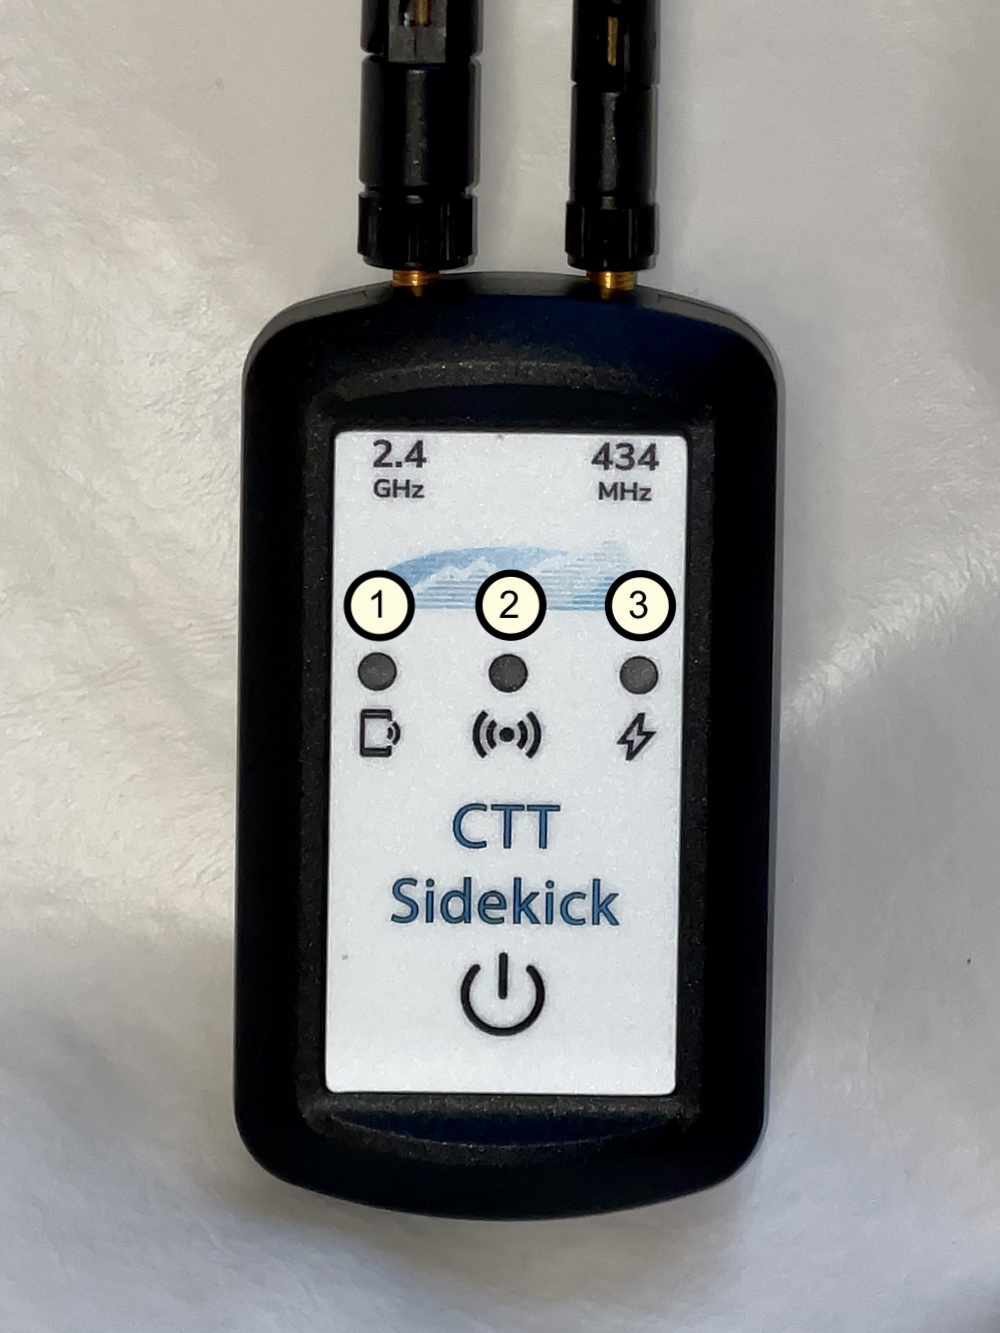
\includegraphics[width=0.25\textwidth,height=\textheight]{./images/Sidekick_LEDs.jpg}
\caption{CTT Sidekick LEDs}\label{id}
}
\end{figure}

\hypertarget{battery-and-charging}{%
\section{Battery and Charging}\label{battery-and-charging}}

Each Sidekick contains a 1000 mA-hr LiPo rechargeable battery with
integrated under/over voltage protection. Battery life is as follows:

\begin{itemize}
\tightlist
\item
  Listening for 434MHz: \textbf{50 hours}
\item
  Listening for 2.4GHz: \textbf{72 hours}
\item
  Listening for both 434MHz and 2.4GHz: \textbf{30 hours}
\end{itemize}

You can check the status of your battery on the CTT Mobile app. Your
Sidekick is fully charged at 4.2V. To charge your Sidekick, use the
included USB charging cable. When plugged in, your Sidekick will
automatically turn on if it's not already. The Pairing Indicator will
blink as it searches for available devices (you can pair with your phone
while charging). The Battery Charge Indicator will remain on (solid
green) when the Sidekick is plugged in. The Battery Charge Indicator
will \emph{remain} on as long as the device is plugged in; it does not
turn off once the Sidekick is fully charged. It's important to check the
battery level through the CTT Mobile app.

\hypertarget{antennas}{%
\section{Antennas}\label{antennas}}

Your Sidekick comes with two omnidirectional antennas, one for 434MHz
(10.5cm) and one for 2.4GHz (19.5cm). Depending on your application, you
can use both antennas simultaneously, or you can opt to connect only
one. Make sure to connect each antenna to it's corresponding port:
\textbf{The longer antenna is for 2.4GHz devices while the shorter
antenna is for 434MHz.}

You may have purchased our optional Yagi antenna(s) and handle(s). These
can used in place of the standard omni antenna by connecting them to
their corresponding antenna port and sliding the Sidekick into the
custom handle.

\begin{figure}
\hypertarget{id}{%
\centering
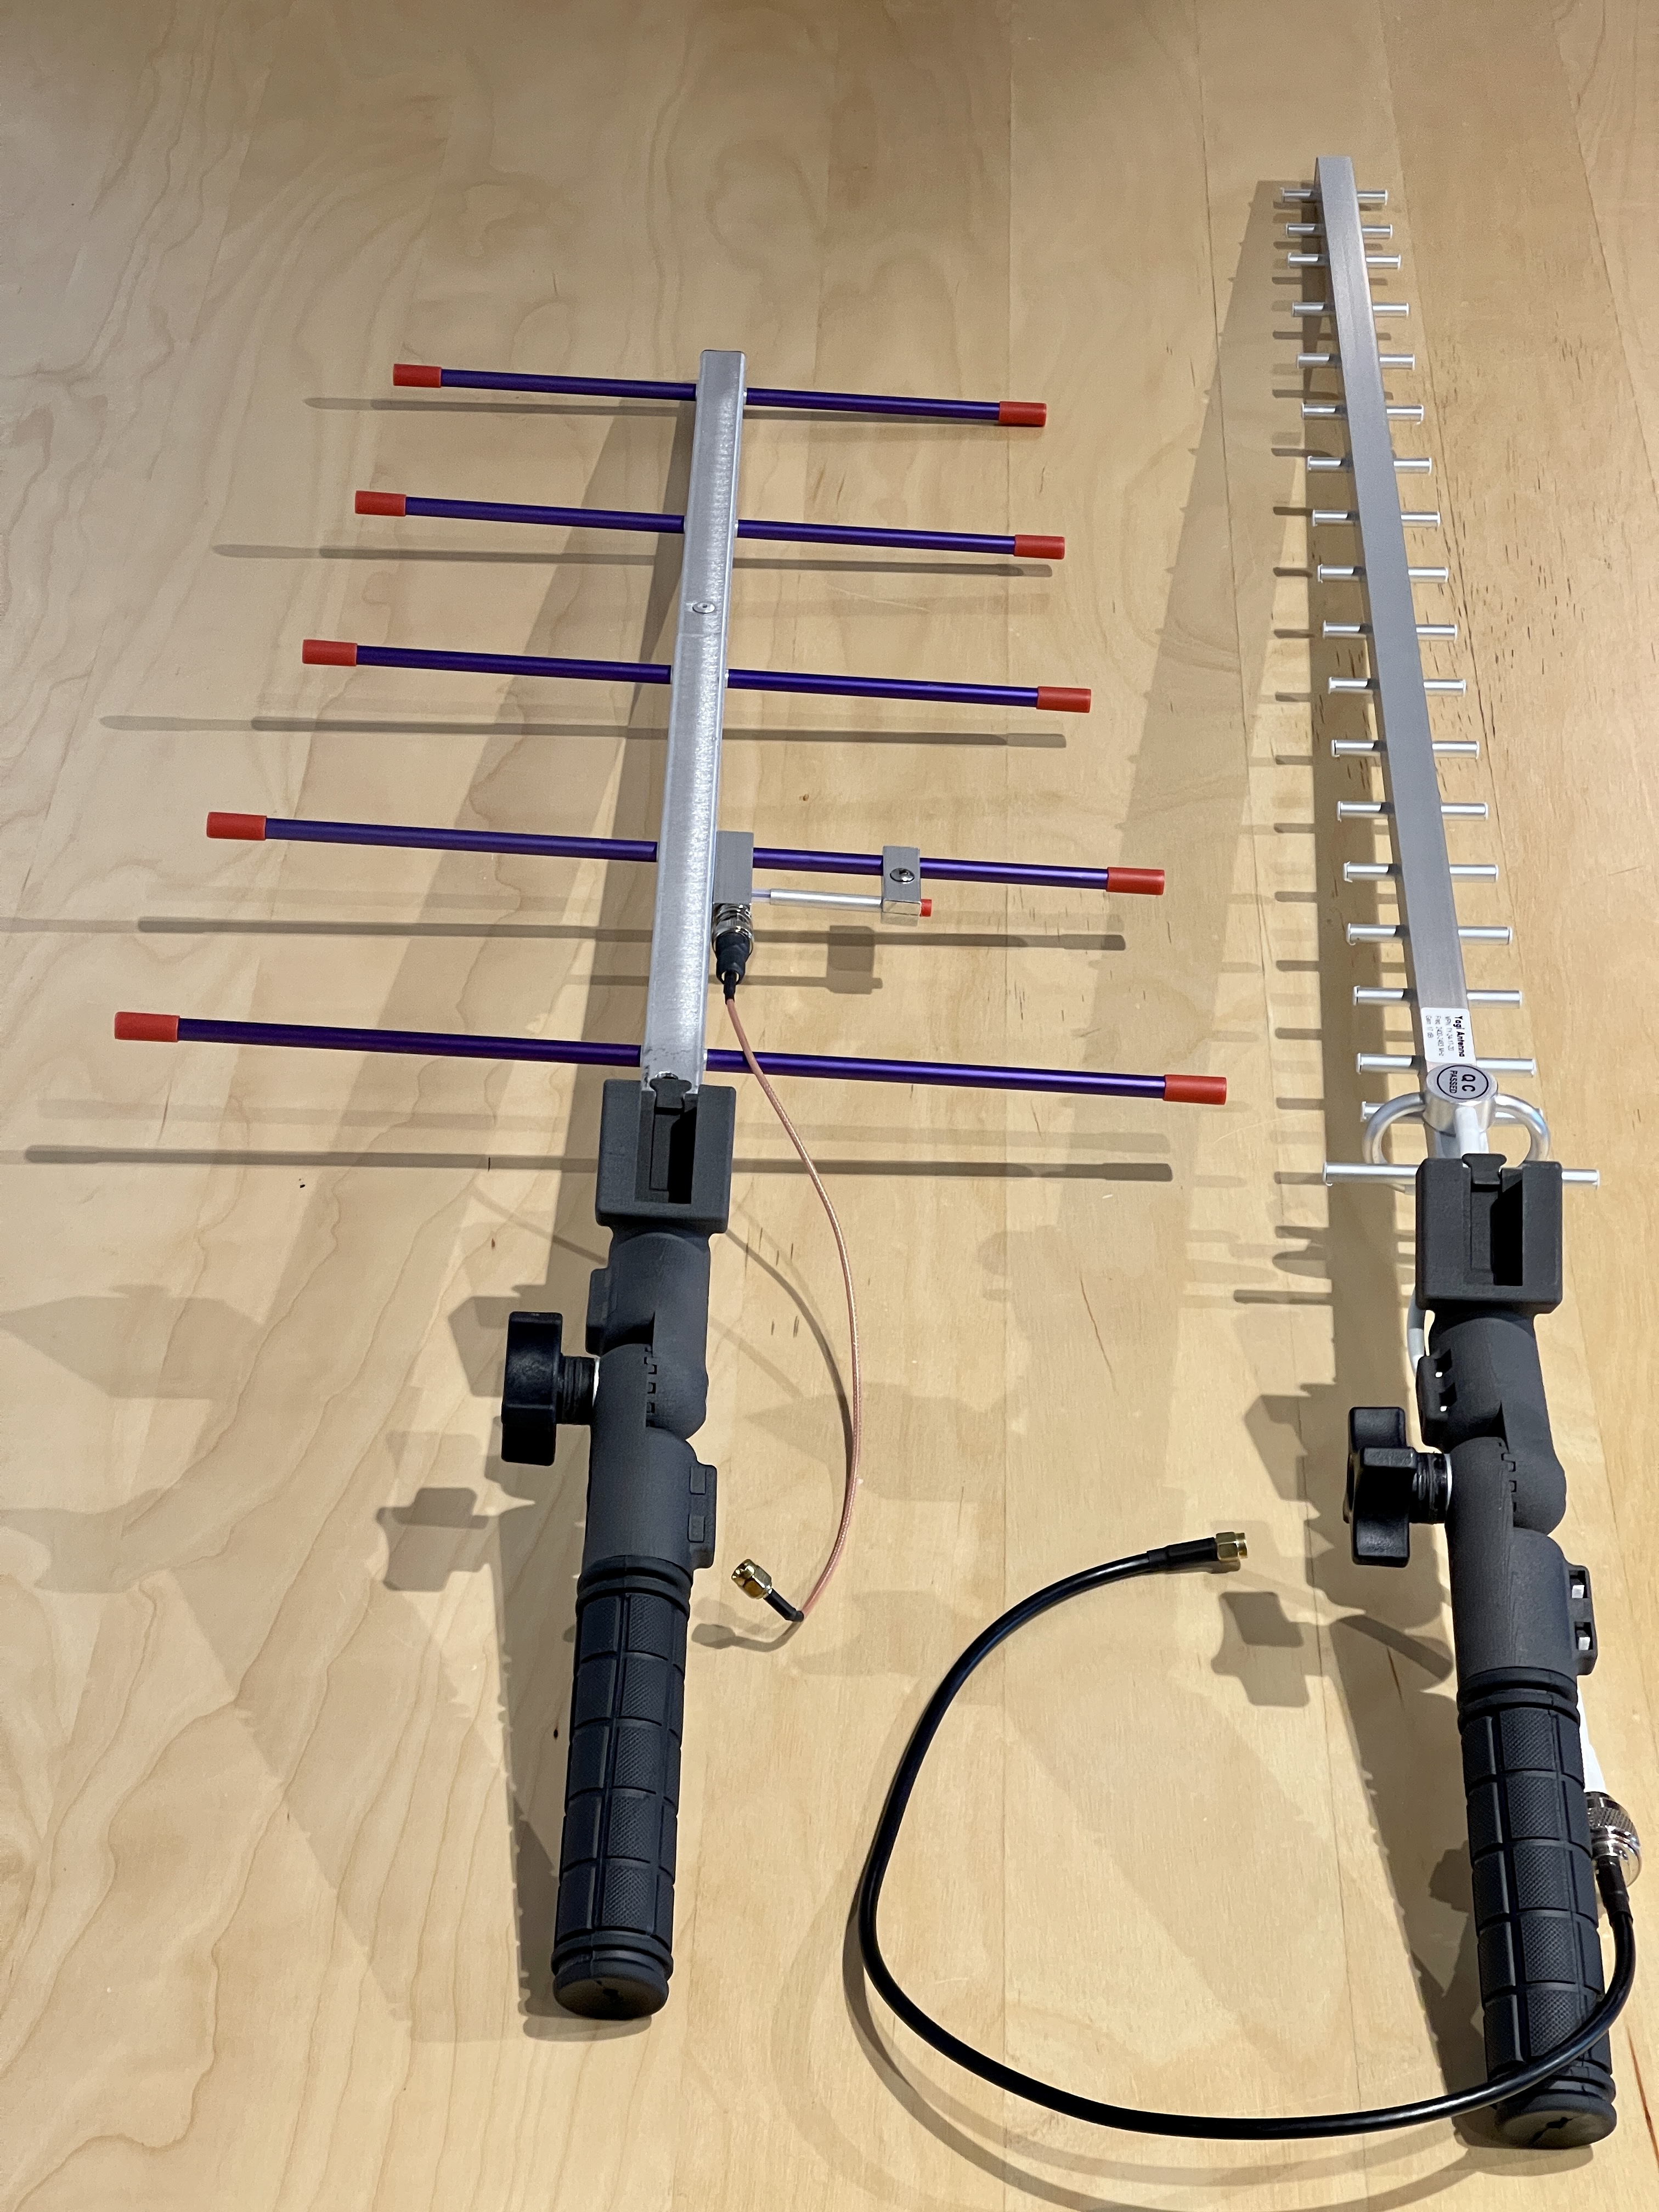
\includegraphics[width=0.5\textwidth,height=\textheight]{./images/sidekick_yagiAntennas.JPG}
\caption{Optional Yagi Antennas and Handles. 434MHz (left) and 2.4GHz
(right)}\label{id}
}
\end{figure}

\begin{figure}
\hypertarget{id}{%
\centering
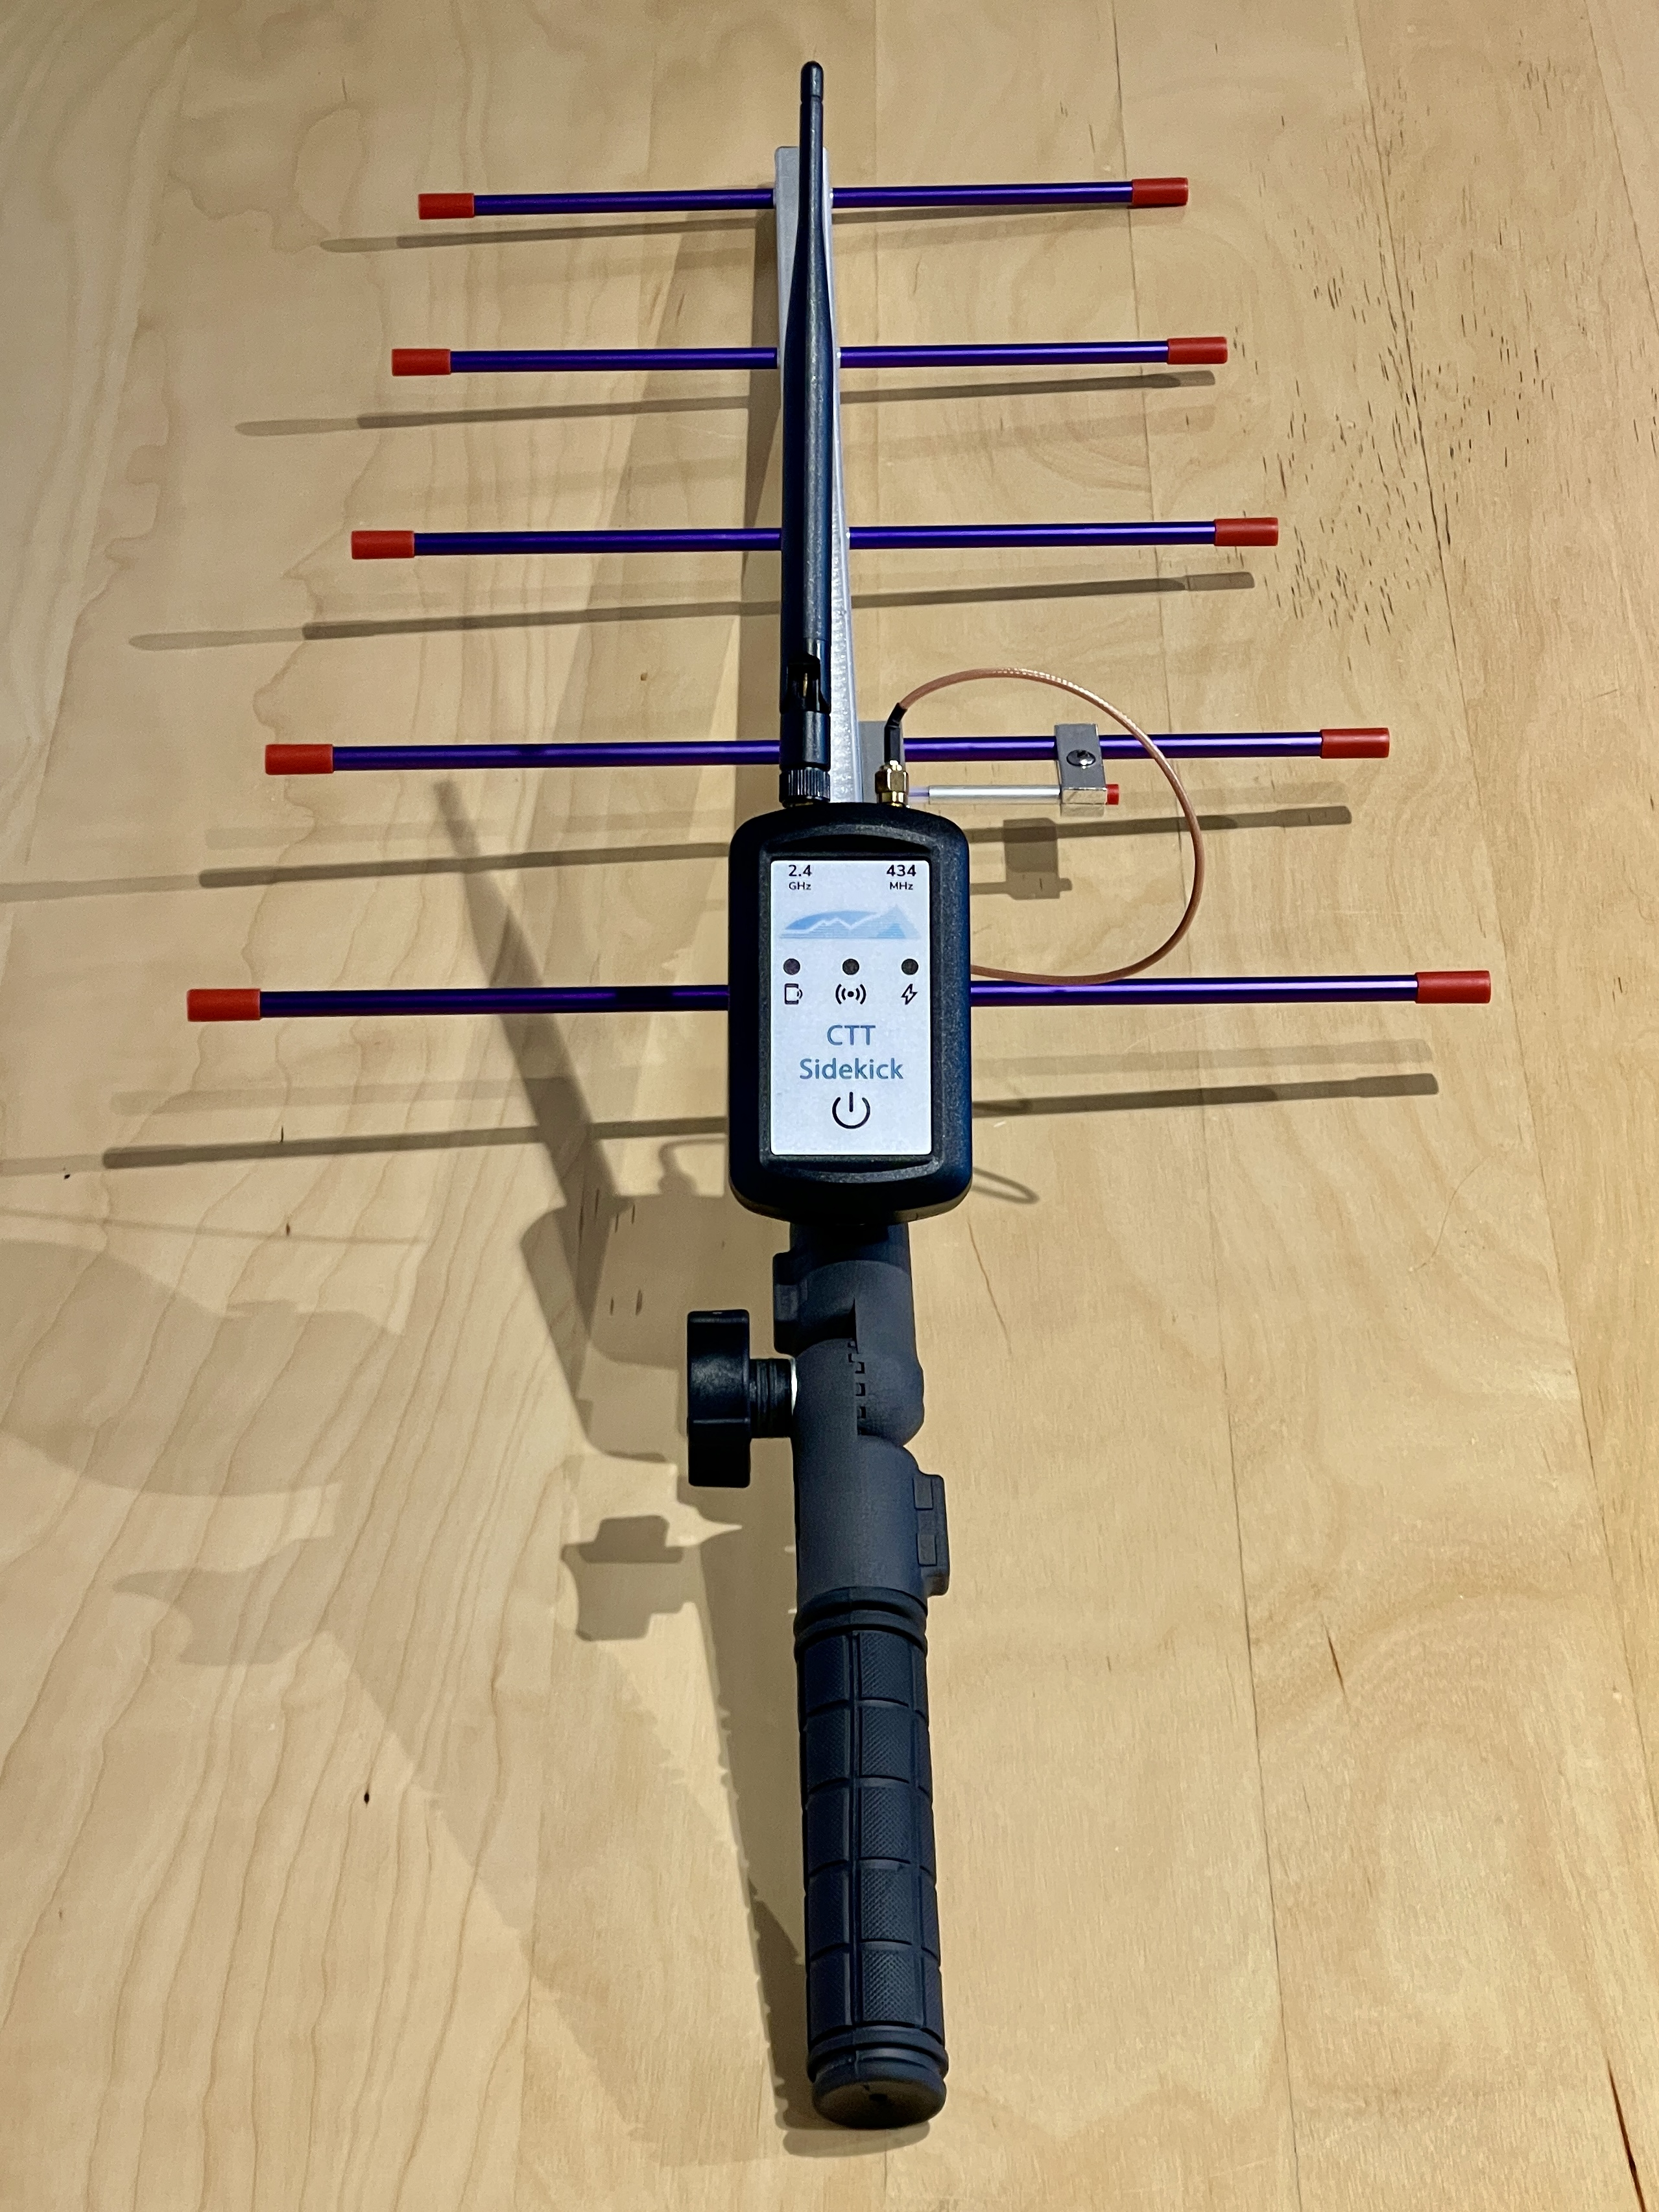
\includegraphics[width=0.5\textwidth,height=\textheight]{./images/sidekick_434MHzYagi.JPG}
\caption{Optional 434MHz Yagi and custom handle with Sidekick locked in.
\emph{Also note the 2.4GHz omni antenna still attached.}}\label{id}
}
\end{figure}

\hypertarget{storing-your-sidekick}{%
\subsection{Storing your Sidekick}\label{storing-your-sidekick}}

While your CTT Sidekick is very robust and field-tested, we recommend
storing your Sidekick with the antennas disconnected from the SMA ports
to avoid any unintended and excessive pressure on the connectors. As
well, you should also use the two dust covers to protect your SMA ports
when not in use.

\hypertarget{mobile-application---ctt-mobile}{%
\section{Mobile Application - CTT
Mobile}\label{mobile-application---ctt-mobile}}

To use the CTT Sidekick, you will need to install the CTT Mobile app on
your Android or iOS device. CTT Mobile is your working interface with
the CTT Sidekick.

\hypertarget{installing-ctt-mobile}{%
\subsection{Installing CTT Mobile}\label{installing-ctt-mobile}}

CTT Mobile is available for download on the iOS AppStore and Google
PlayStore.

\hypertarget{pairing-with-ctt-sidekick}{%
\subsection{Pairing with CTT Sidekick}\label{pairing-with-ctt-sidekick}}

To begin using your CTT Sidekick, you'll need to pair your smartphone
(or other smart device) to the Sidekick using the CTT Mobile app. Please
follow the instructions below:

\begin{enumerate}
\def\labelenumi{\arabic{enumi}.}
\tightlist
\item
  From the home screen of CTT Mobile, select the Connect Device launch
  tile.
\end{enumerate}

\begin{figure}
\hypertarget{id}{%
\centering
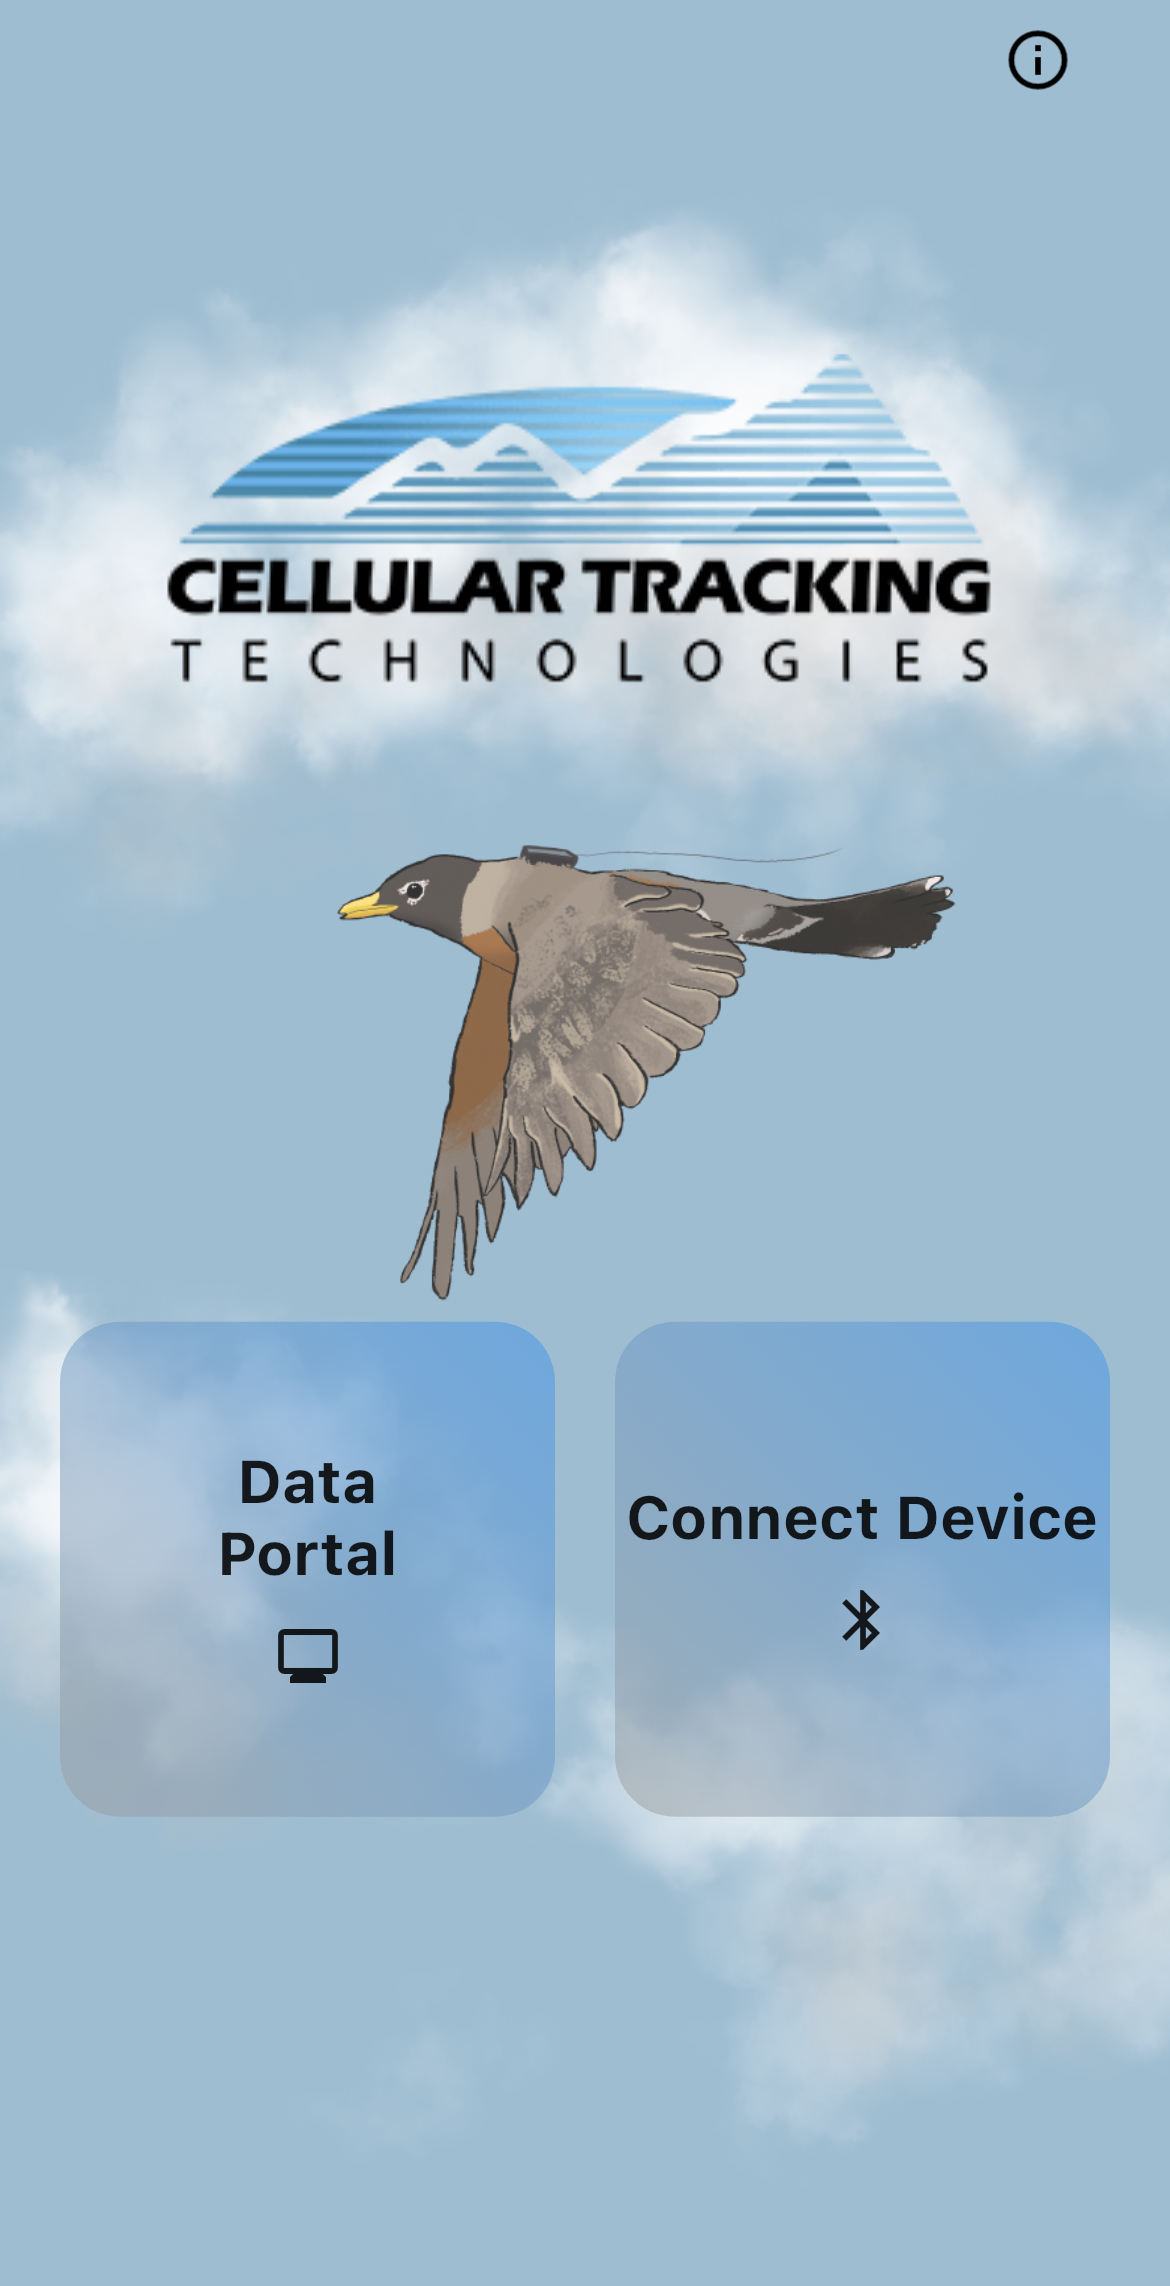
\includegraphics[width=0.25\textwidth,height=\textheight]{./images/CTT Mobile_1.jpg}
\caption{CTT Mobile Home Screen}\label{id}
}
\end{figure}

\begin{enumerate}
\def\labelenumi{\arabic{enumi}.}
\setcounter{enumi}{1}
\tightlist
\item
  Tap the Start Scan button and a list of available devices will appear.
\end{enumerate}

\begin{figure}
\hypertarget{id}{%
\centering
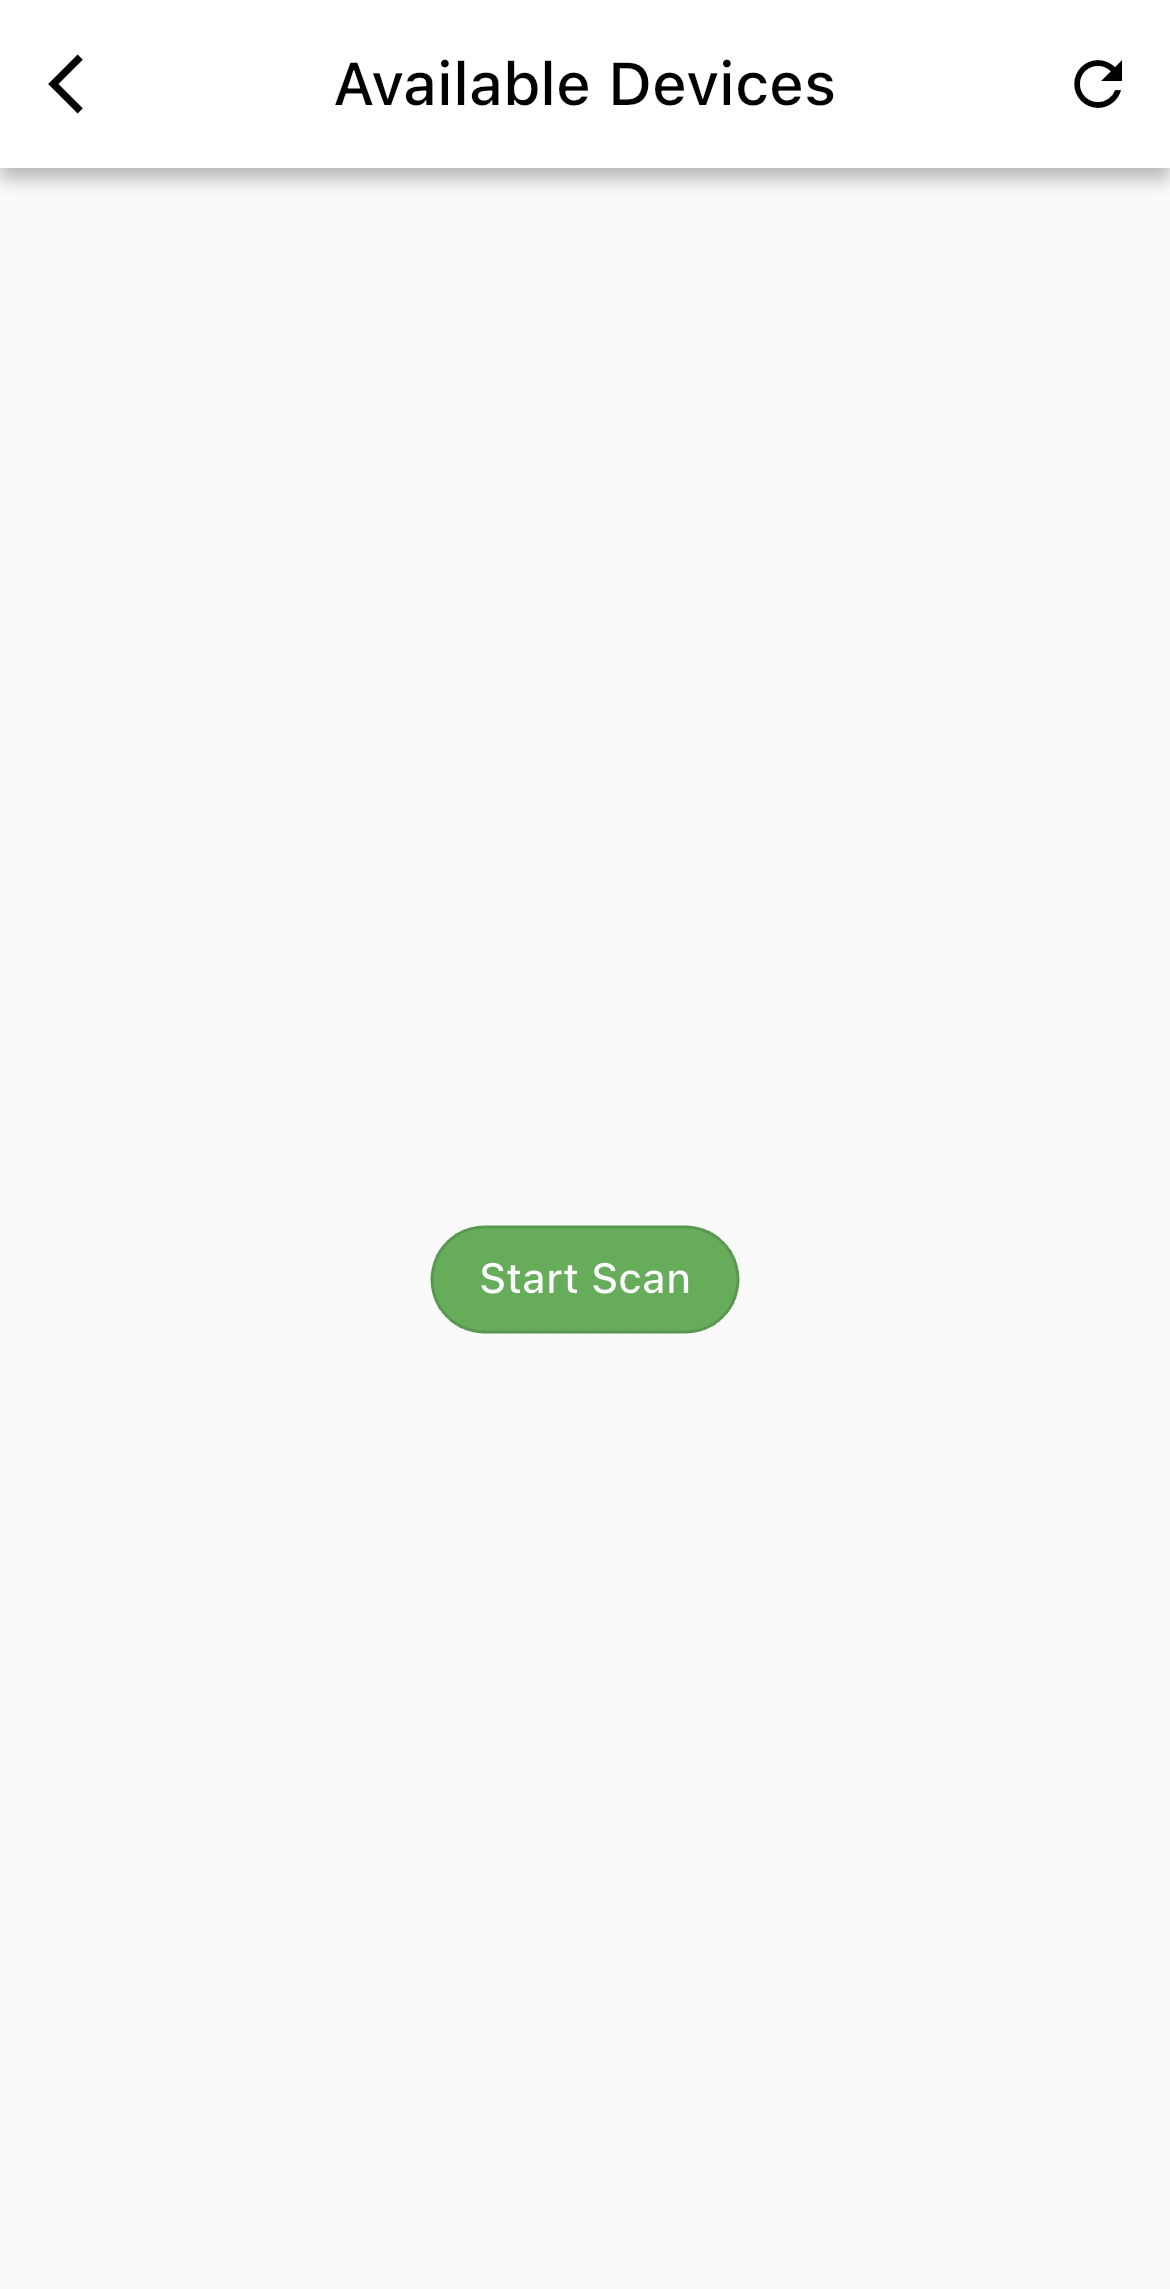
\includegraphics[width=0.25\textwidth,height=\textheight]{./images/CTT Mobile_2.jpg}
\caption{Start Scan Screen}\label{id}
}
\end{figure}

\begin{enumerate}
\def\labelenumi{\arabic{enumi}.}
\setcounter{enumi}{2}
\tightlist
\item
  The CTT Sidekick will be listed as \textbf{CTT Sidekick (XXXXXXXX)} in
  the available devices list, where XXXXXXXX is the unique identifier of
  your CTT Sidekick. Find the your Sidekick in the list and tap Connect.
\end{enumerate}

\begin{figure}
\hypertarget{id}{%
\centering
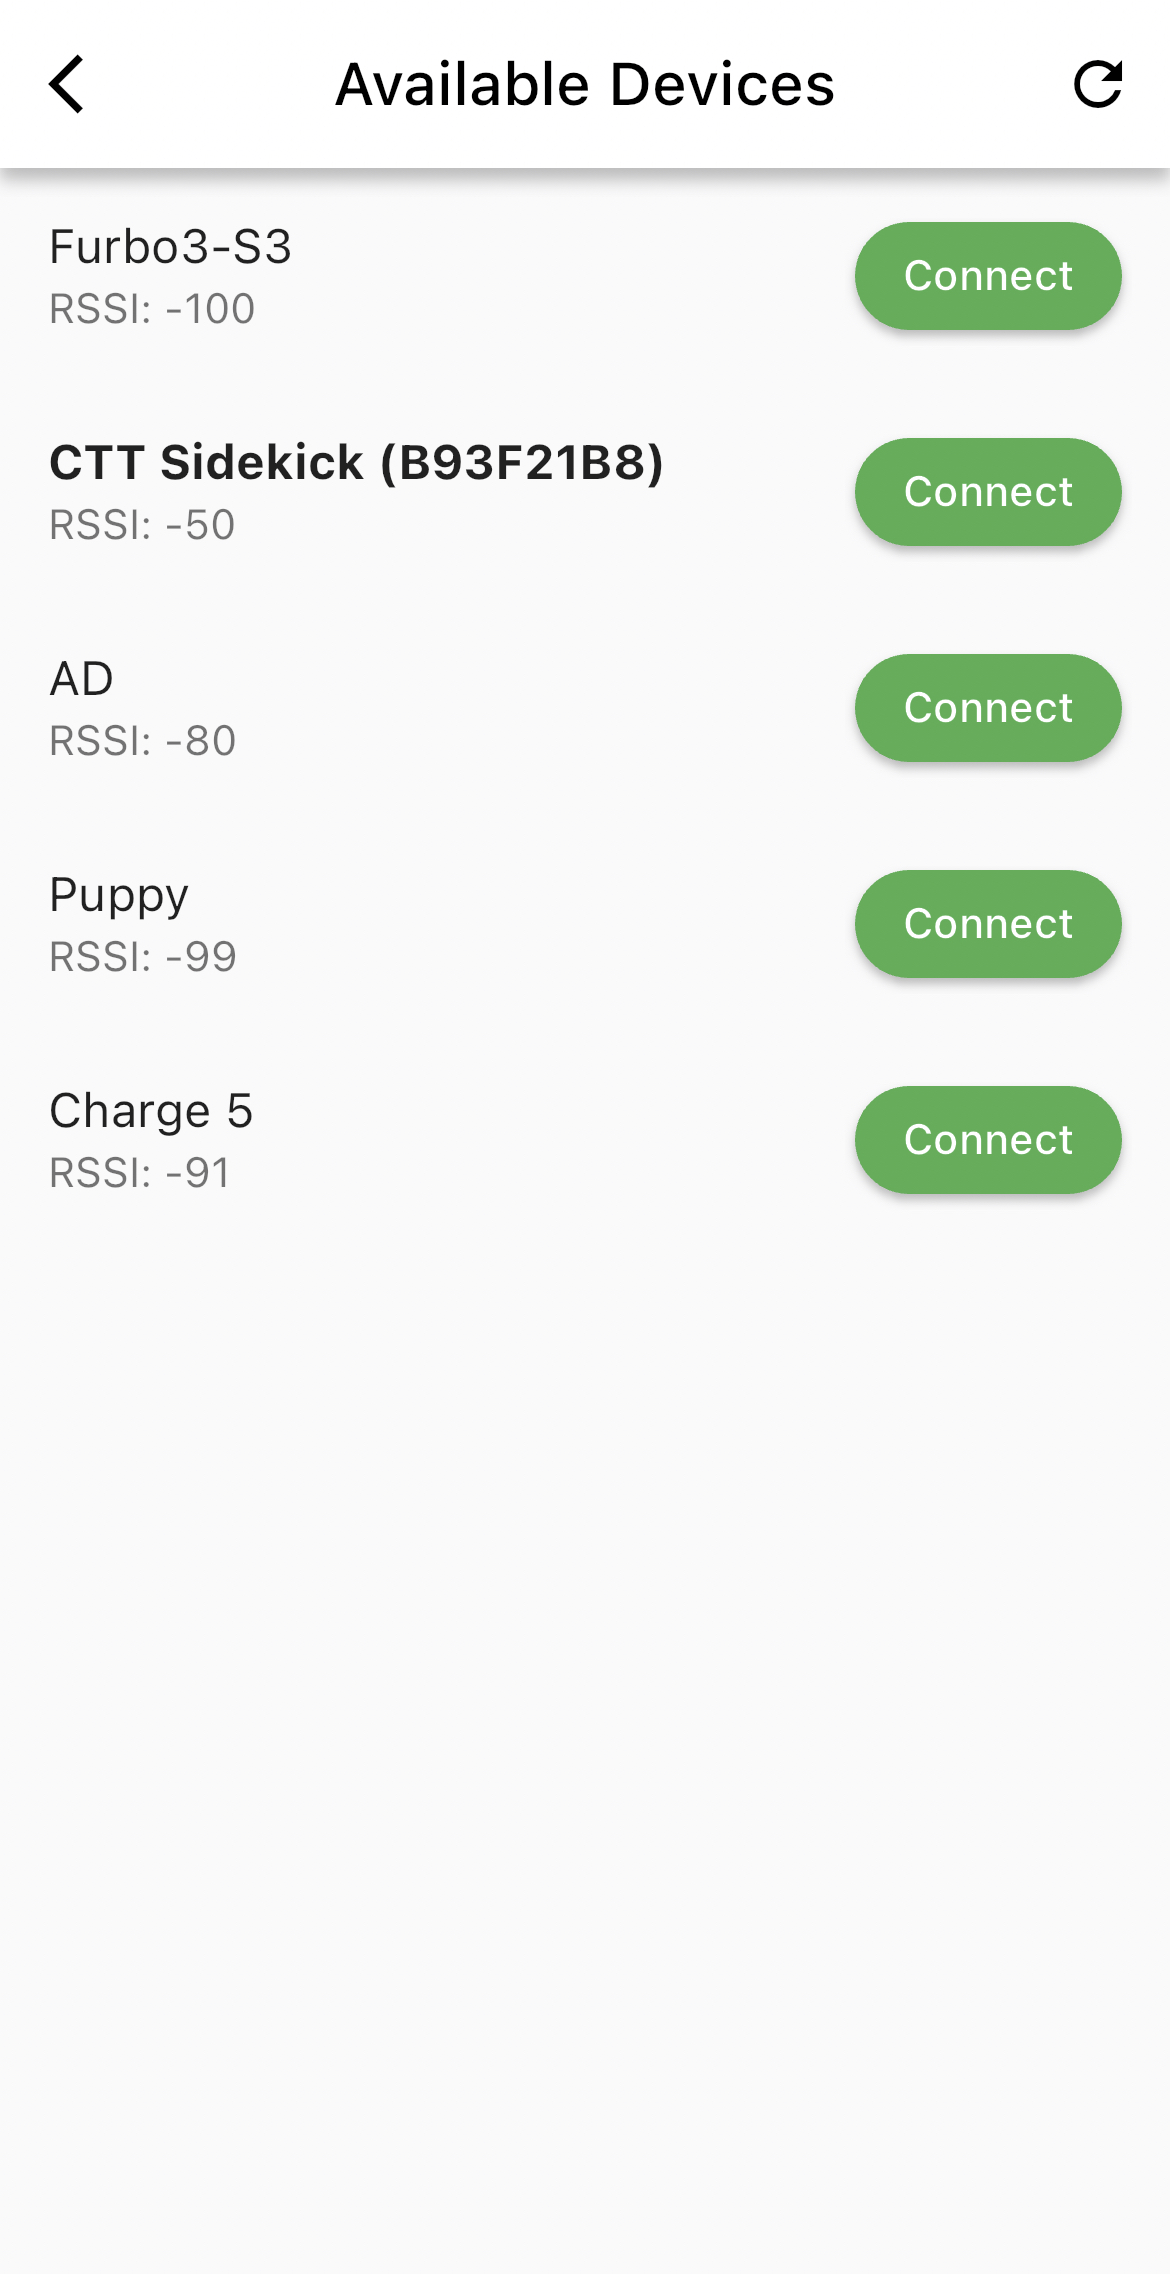
\includegraphics[width=0.25\textwidth,height=\textheight]{./images/CTT Mobile_3.jpg}
\caption{Device Screen}\label{id}
}
\end{figure}

\begin{enumerate}
\def\labelenumi{\arabic{enumi}.}
\setcounter{enumi}{3}
\tightlist
\item
  Once pairing is complete, the mobile application will notify you. Tap
  ``Go'\,' to continue to the CTT Sidekick Main Hub screen.
\end{enumerate}

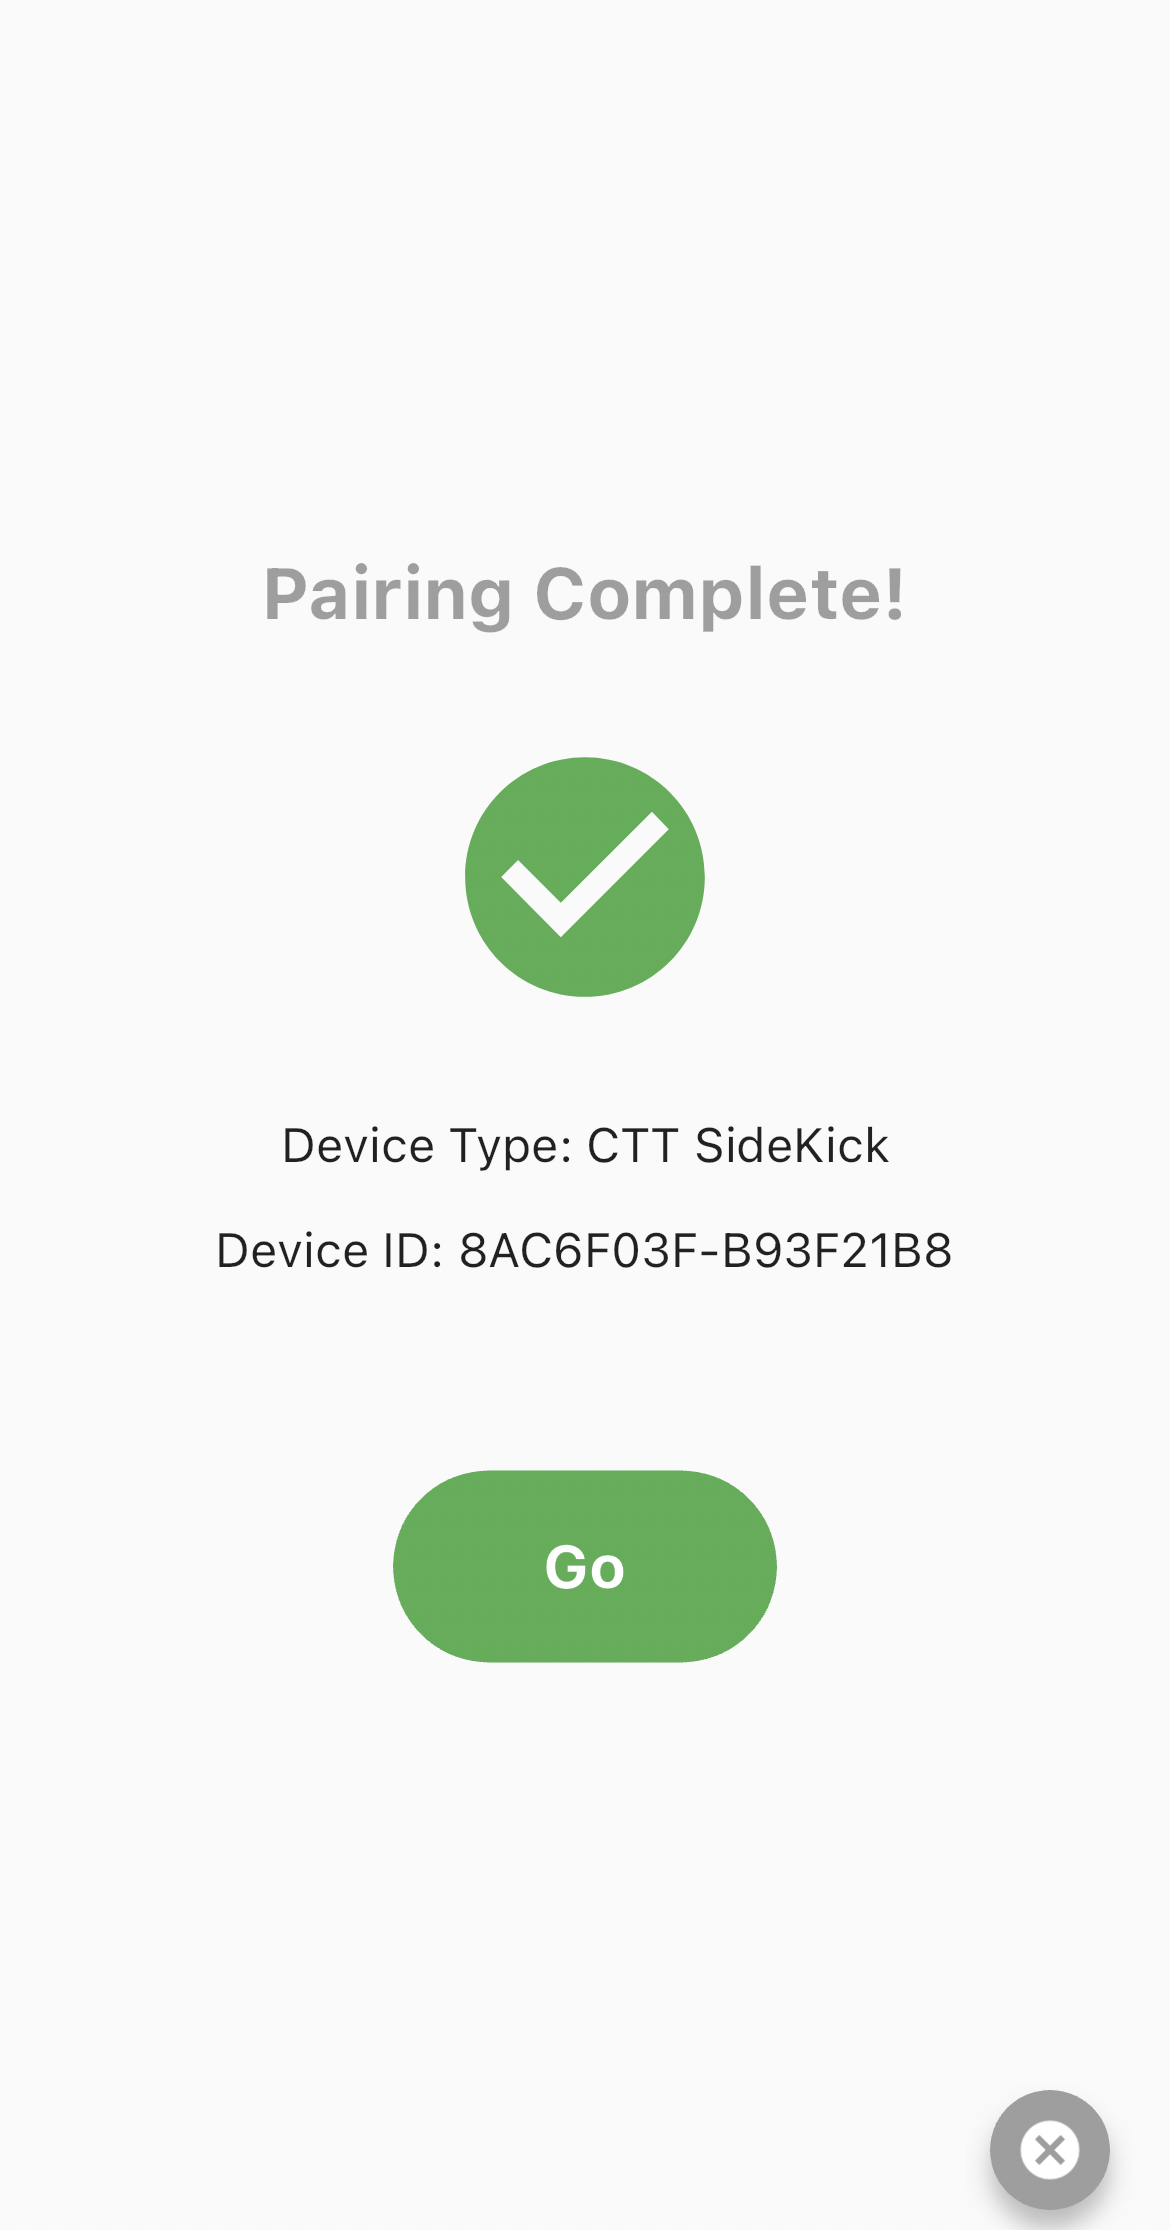
\includegraphics[width=0.25\textwidth,height=\textheight]{./images/CTT Mobile_4.jpg}
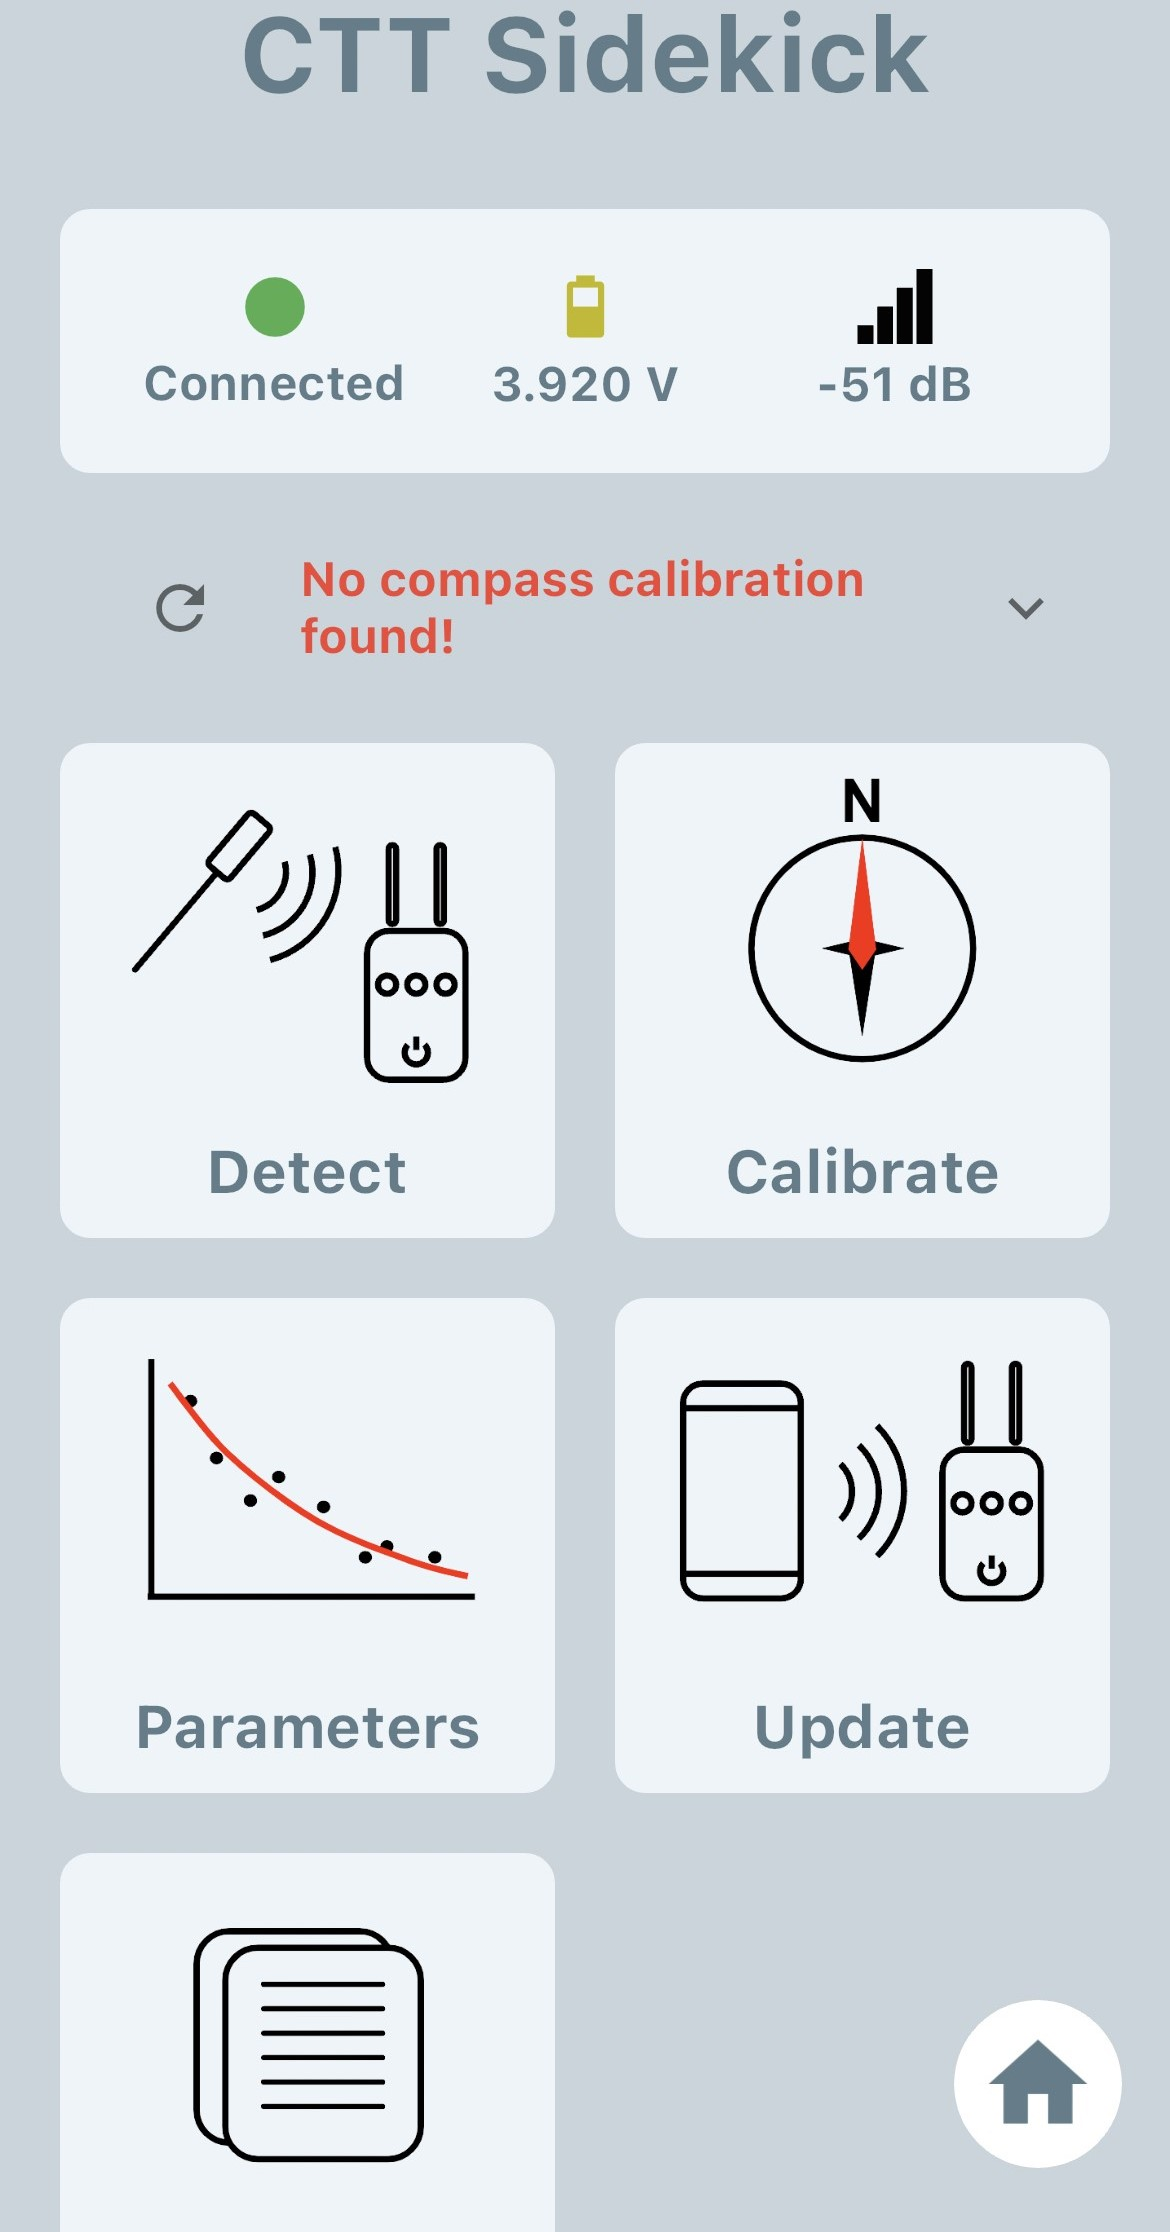
\includegraphics[width=0.25\textwidth,height=\textheight]{./images/CTT Mobile_5.jpg}

\hypertarget{sidekick-operation}{%
\section{Sidekick Operation}\label{sidekick-operation}}

After pairing is complete, you will see the CTT Sidekick Main Hub screen
(see figure above). Please note, the Home button at the bottom right
will exit the Sidekick Hub and return you to the homescreen for CTT
Mobile. You will need to reconnect to your Sidekick from there.

\hypertarget{calibrate-compass}{%
\subsection{Calibrate Compass}\label{calibrate-compass}}

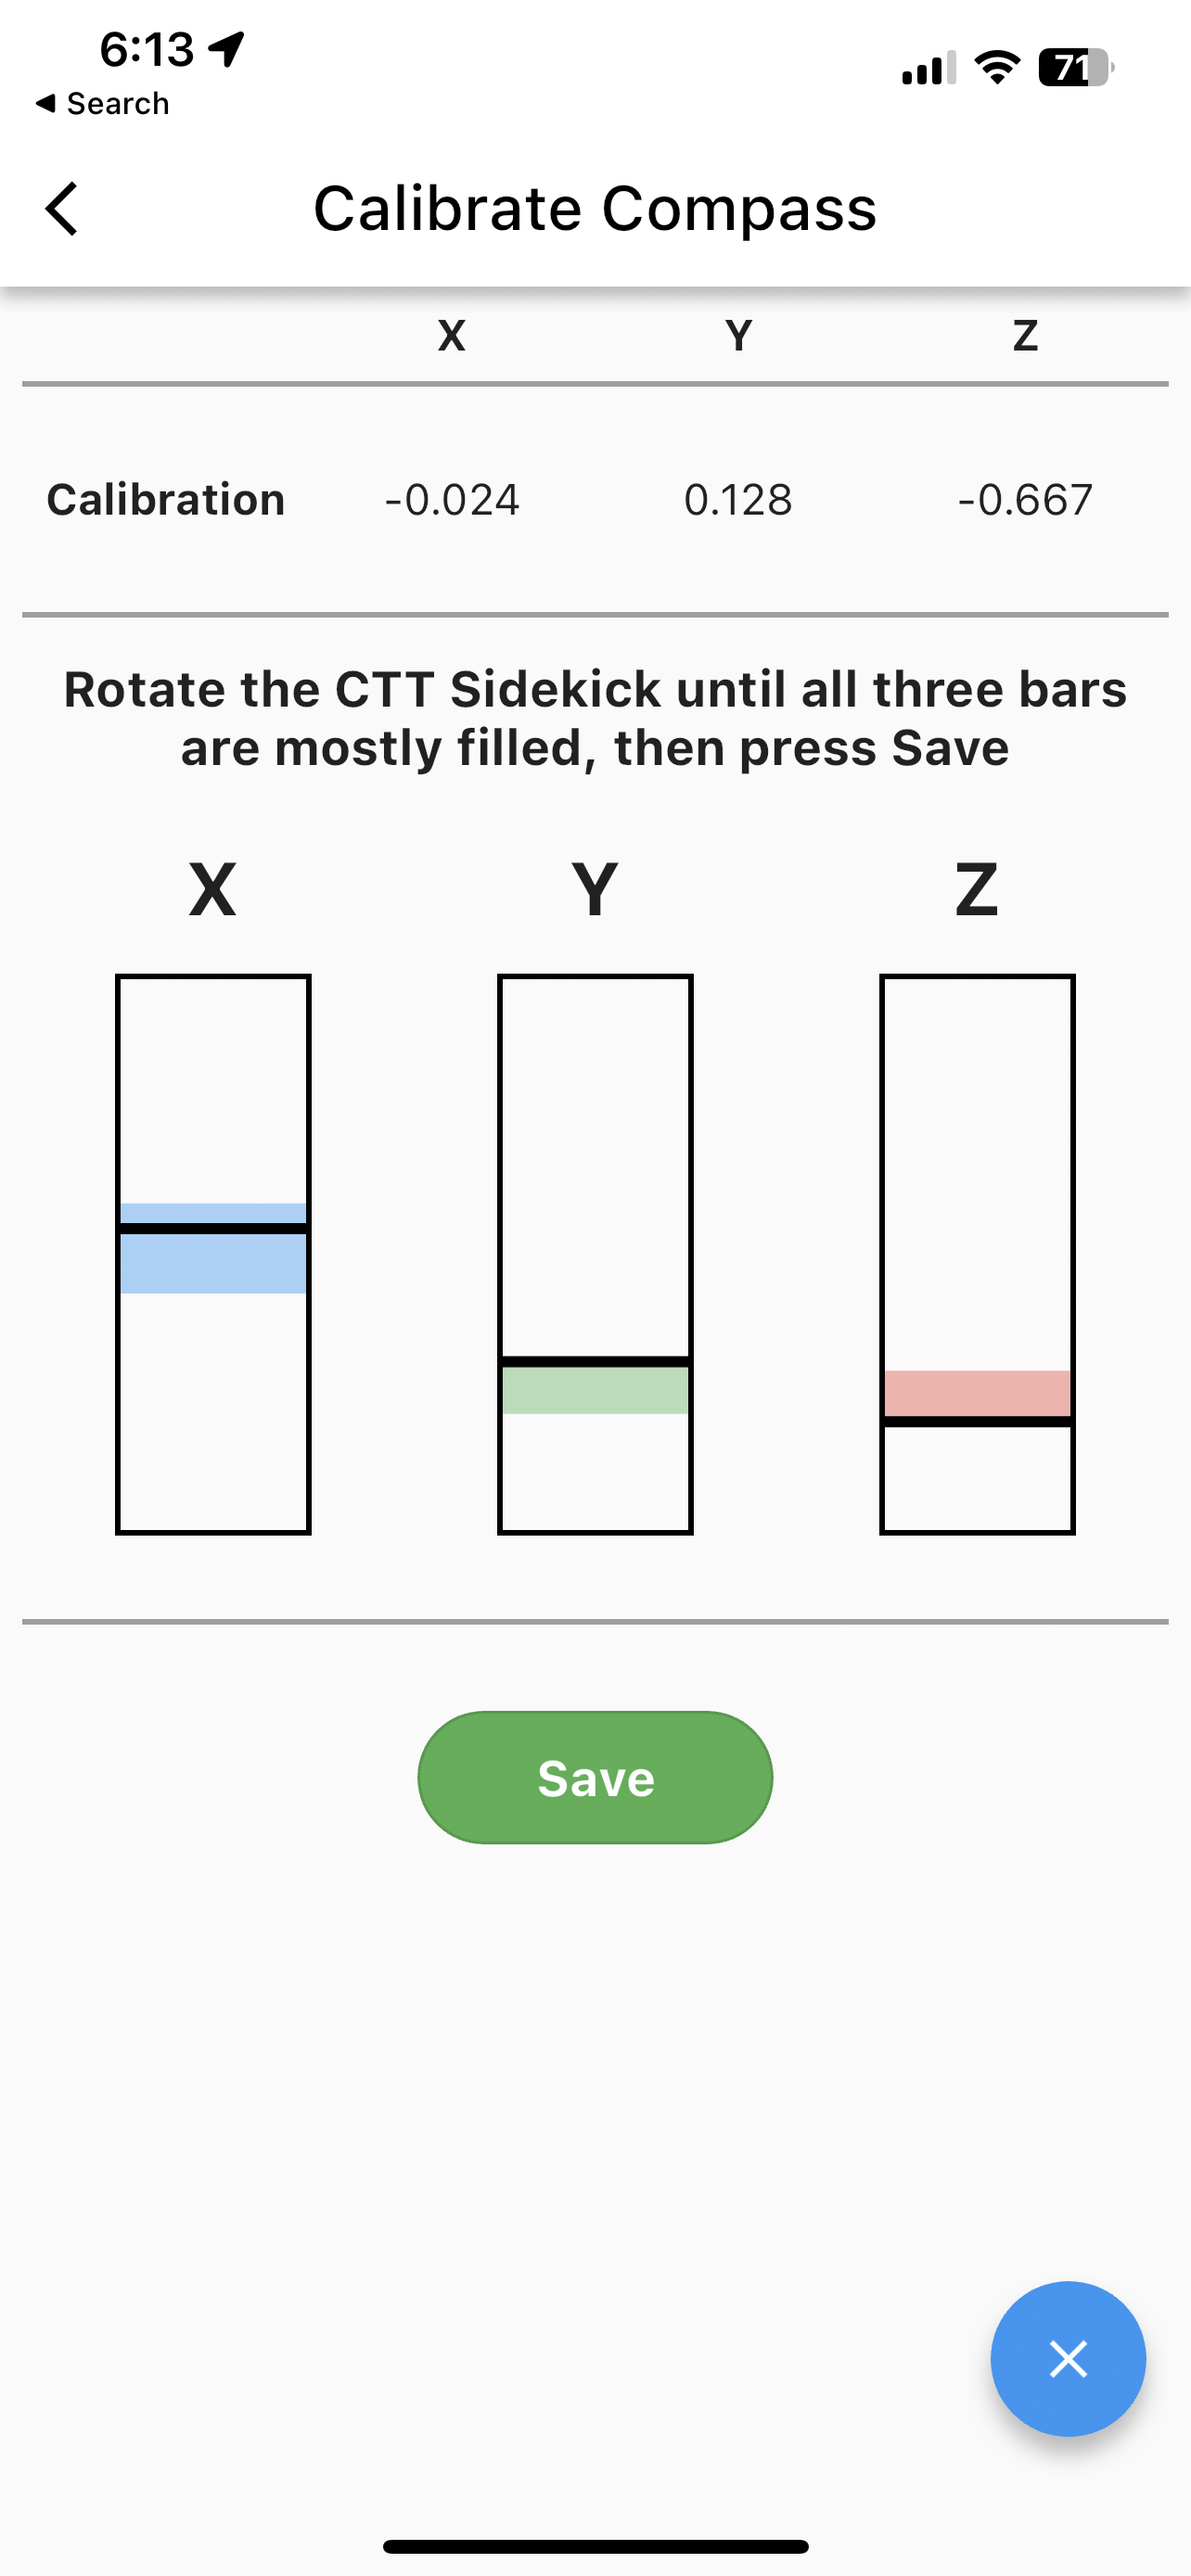
\includegraphics[width=0.25\textwidth,height=\textheight]{./images/sidekick_compassCalib1.PNG}
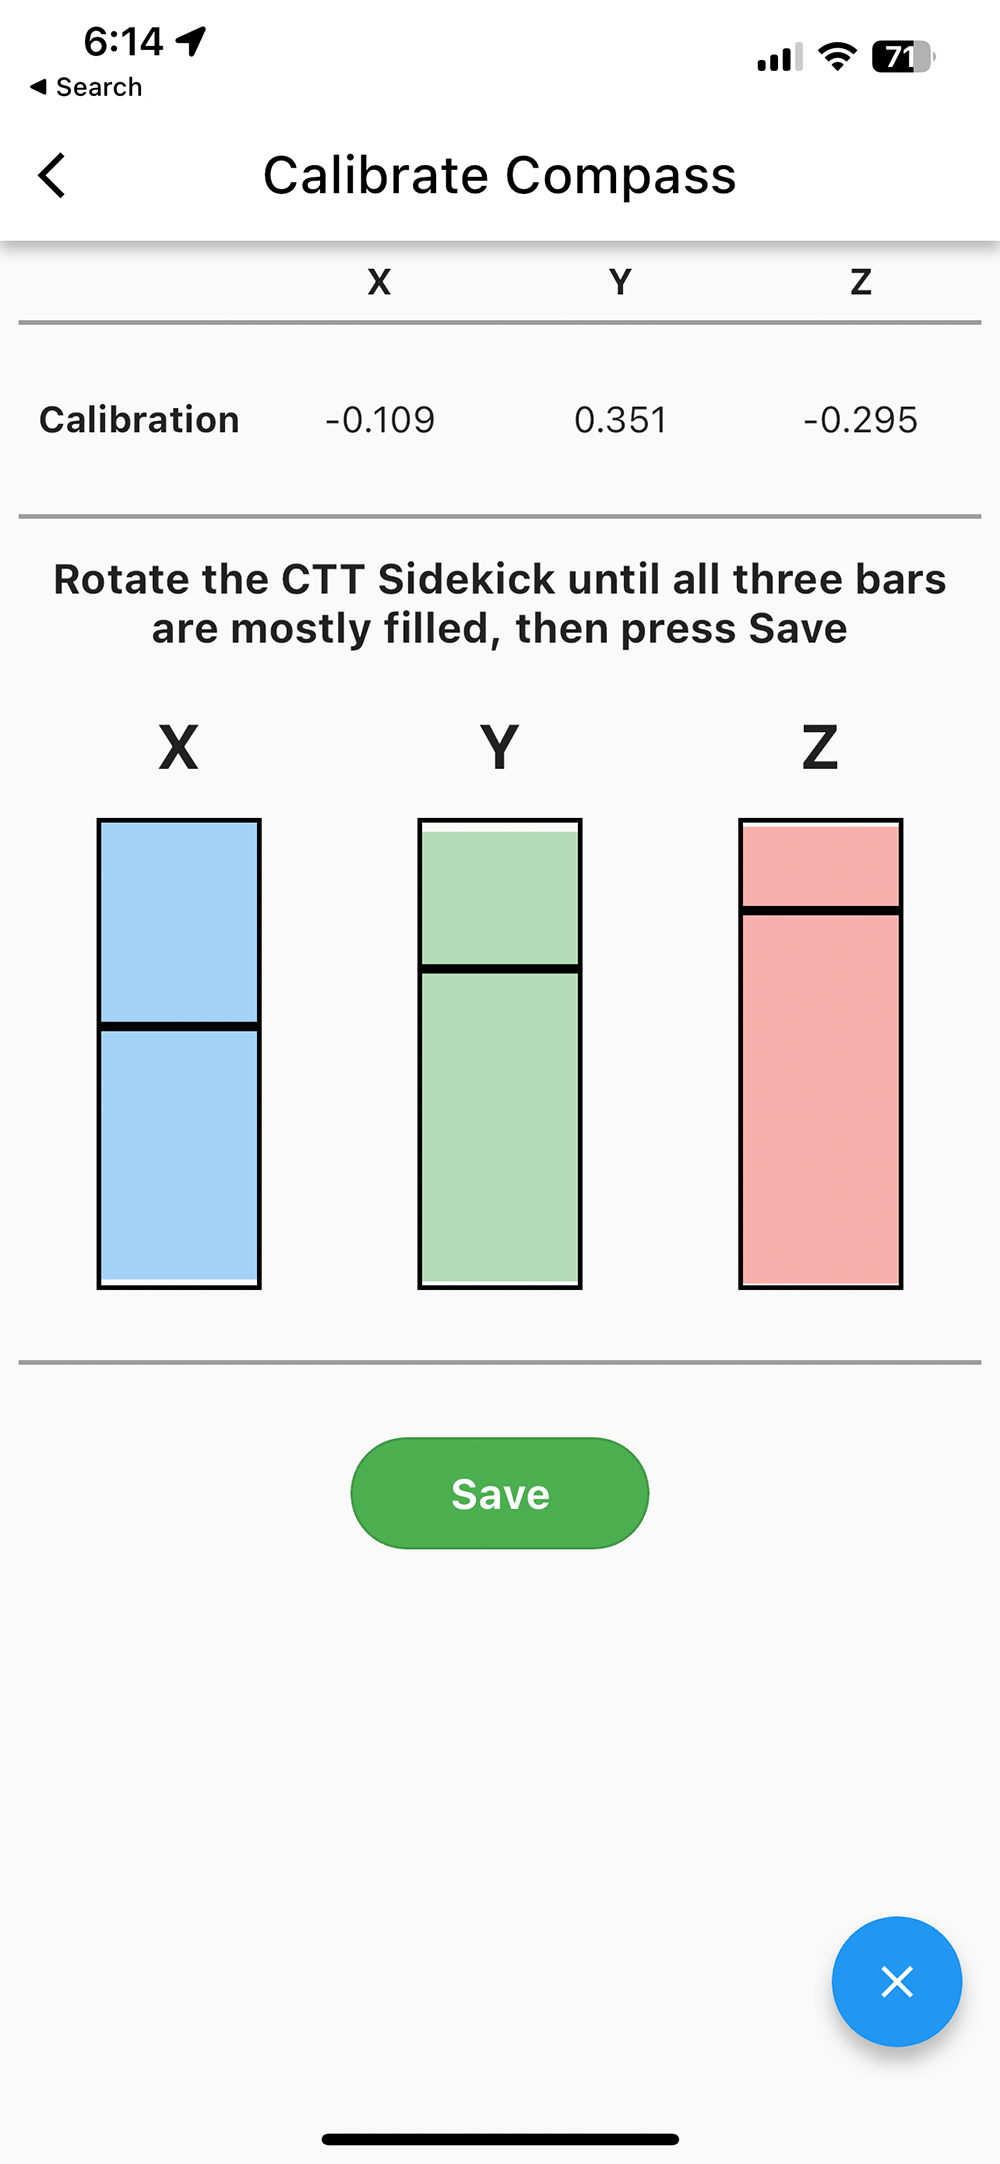
\includegraphics[width=0.25\textwidth,height=\textheight]{./images/sidekick_compassCalib2.PNG}
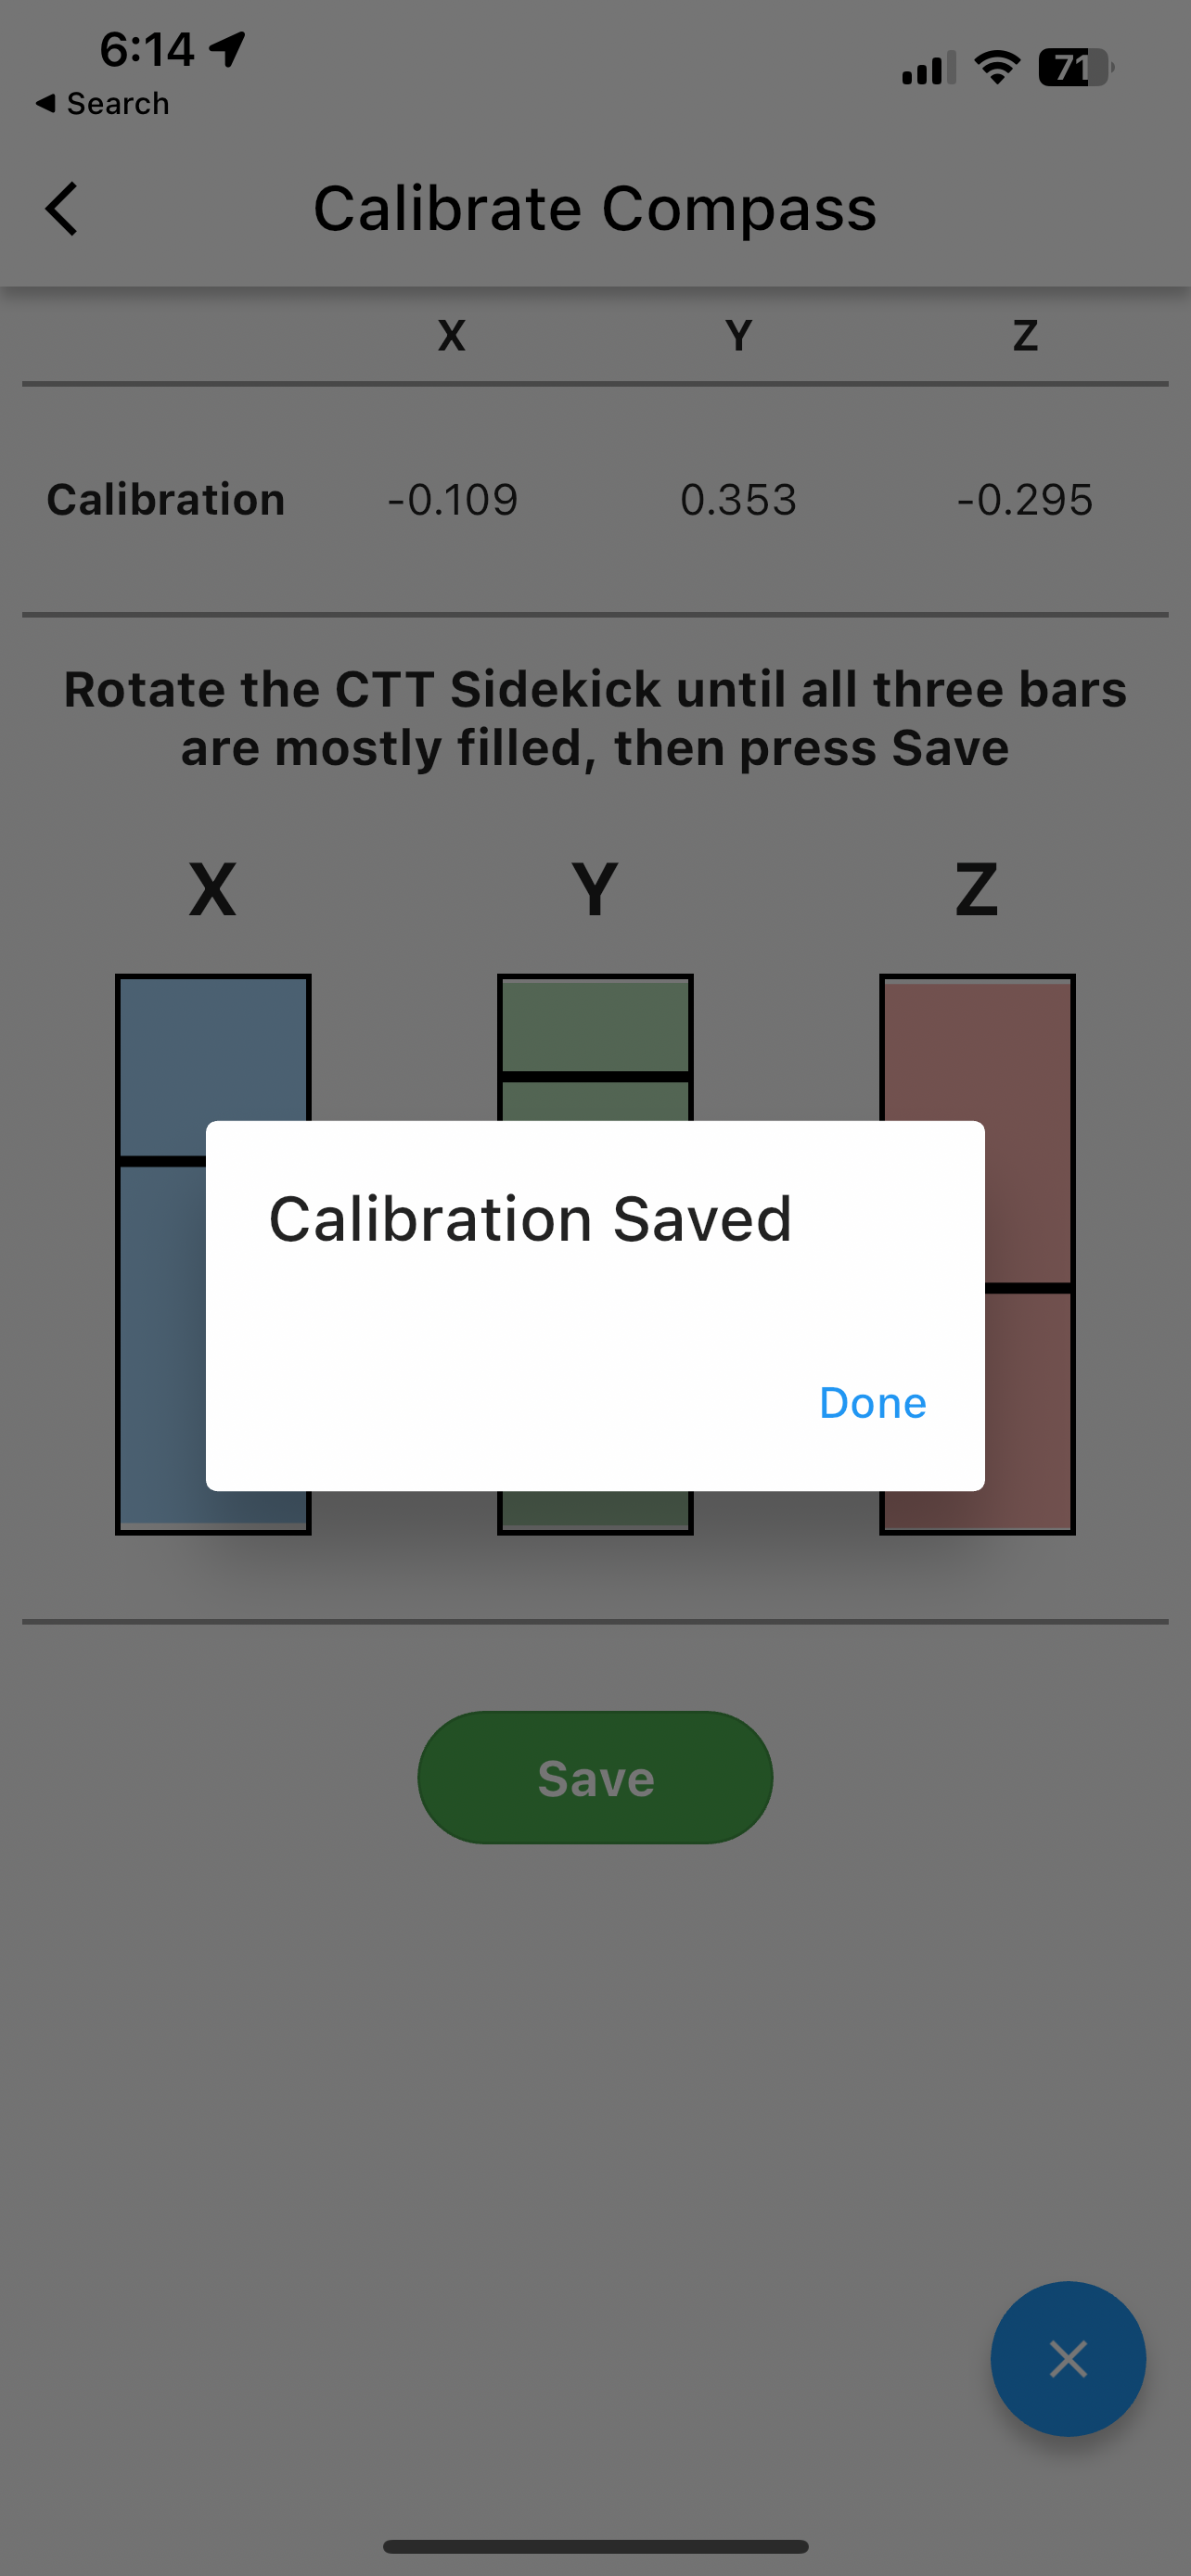
\includegraphics[width=0.25\textwidth,height=\textheight]{./images/sidekick_calibrationSaved.PNG}

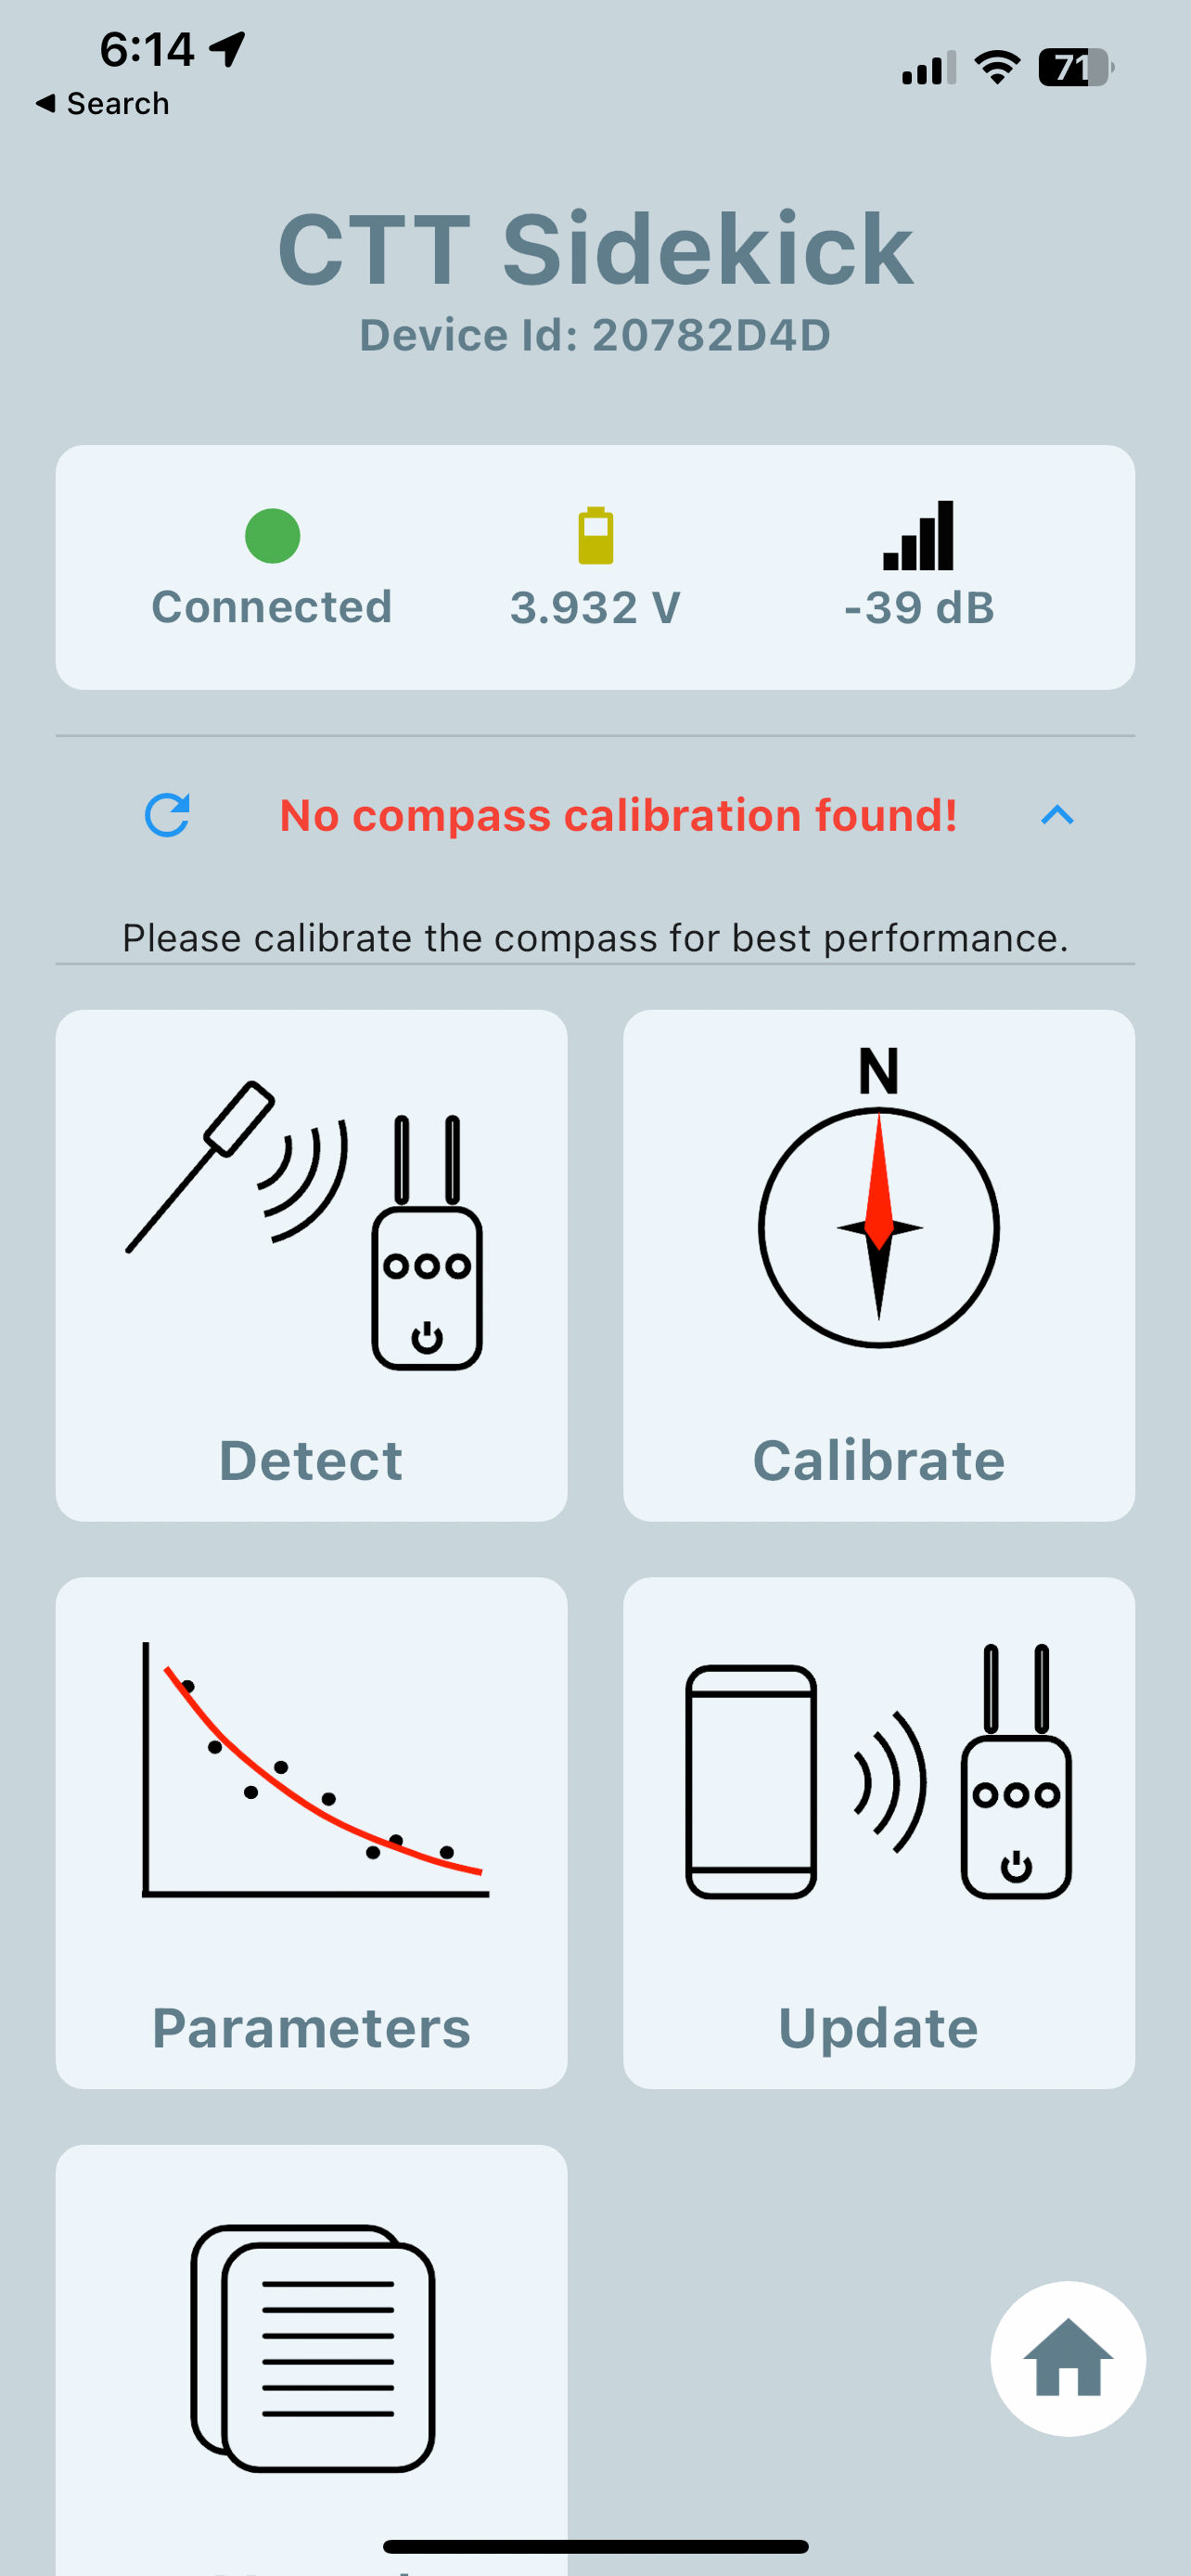
\includegraphics[width=0.25\textwidth,height=\textheight]{./images/sidekick_CompassNotCalib.PNG}
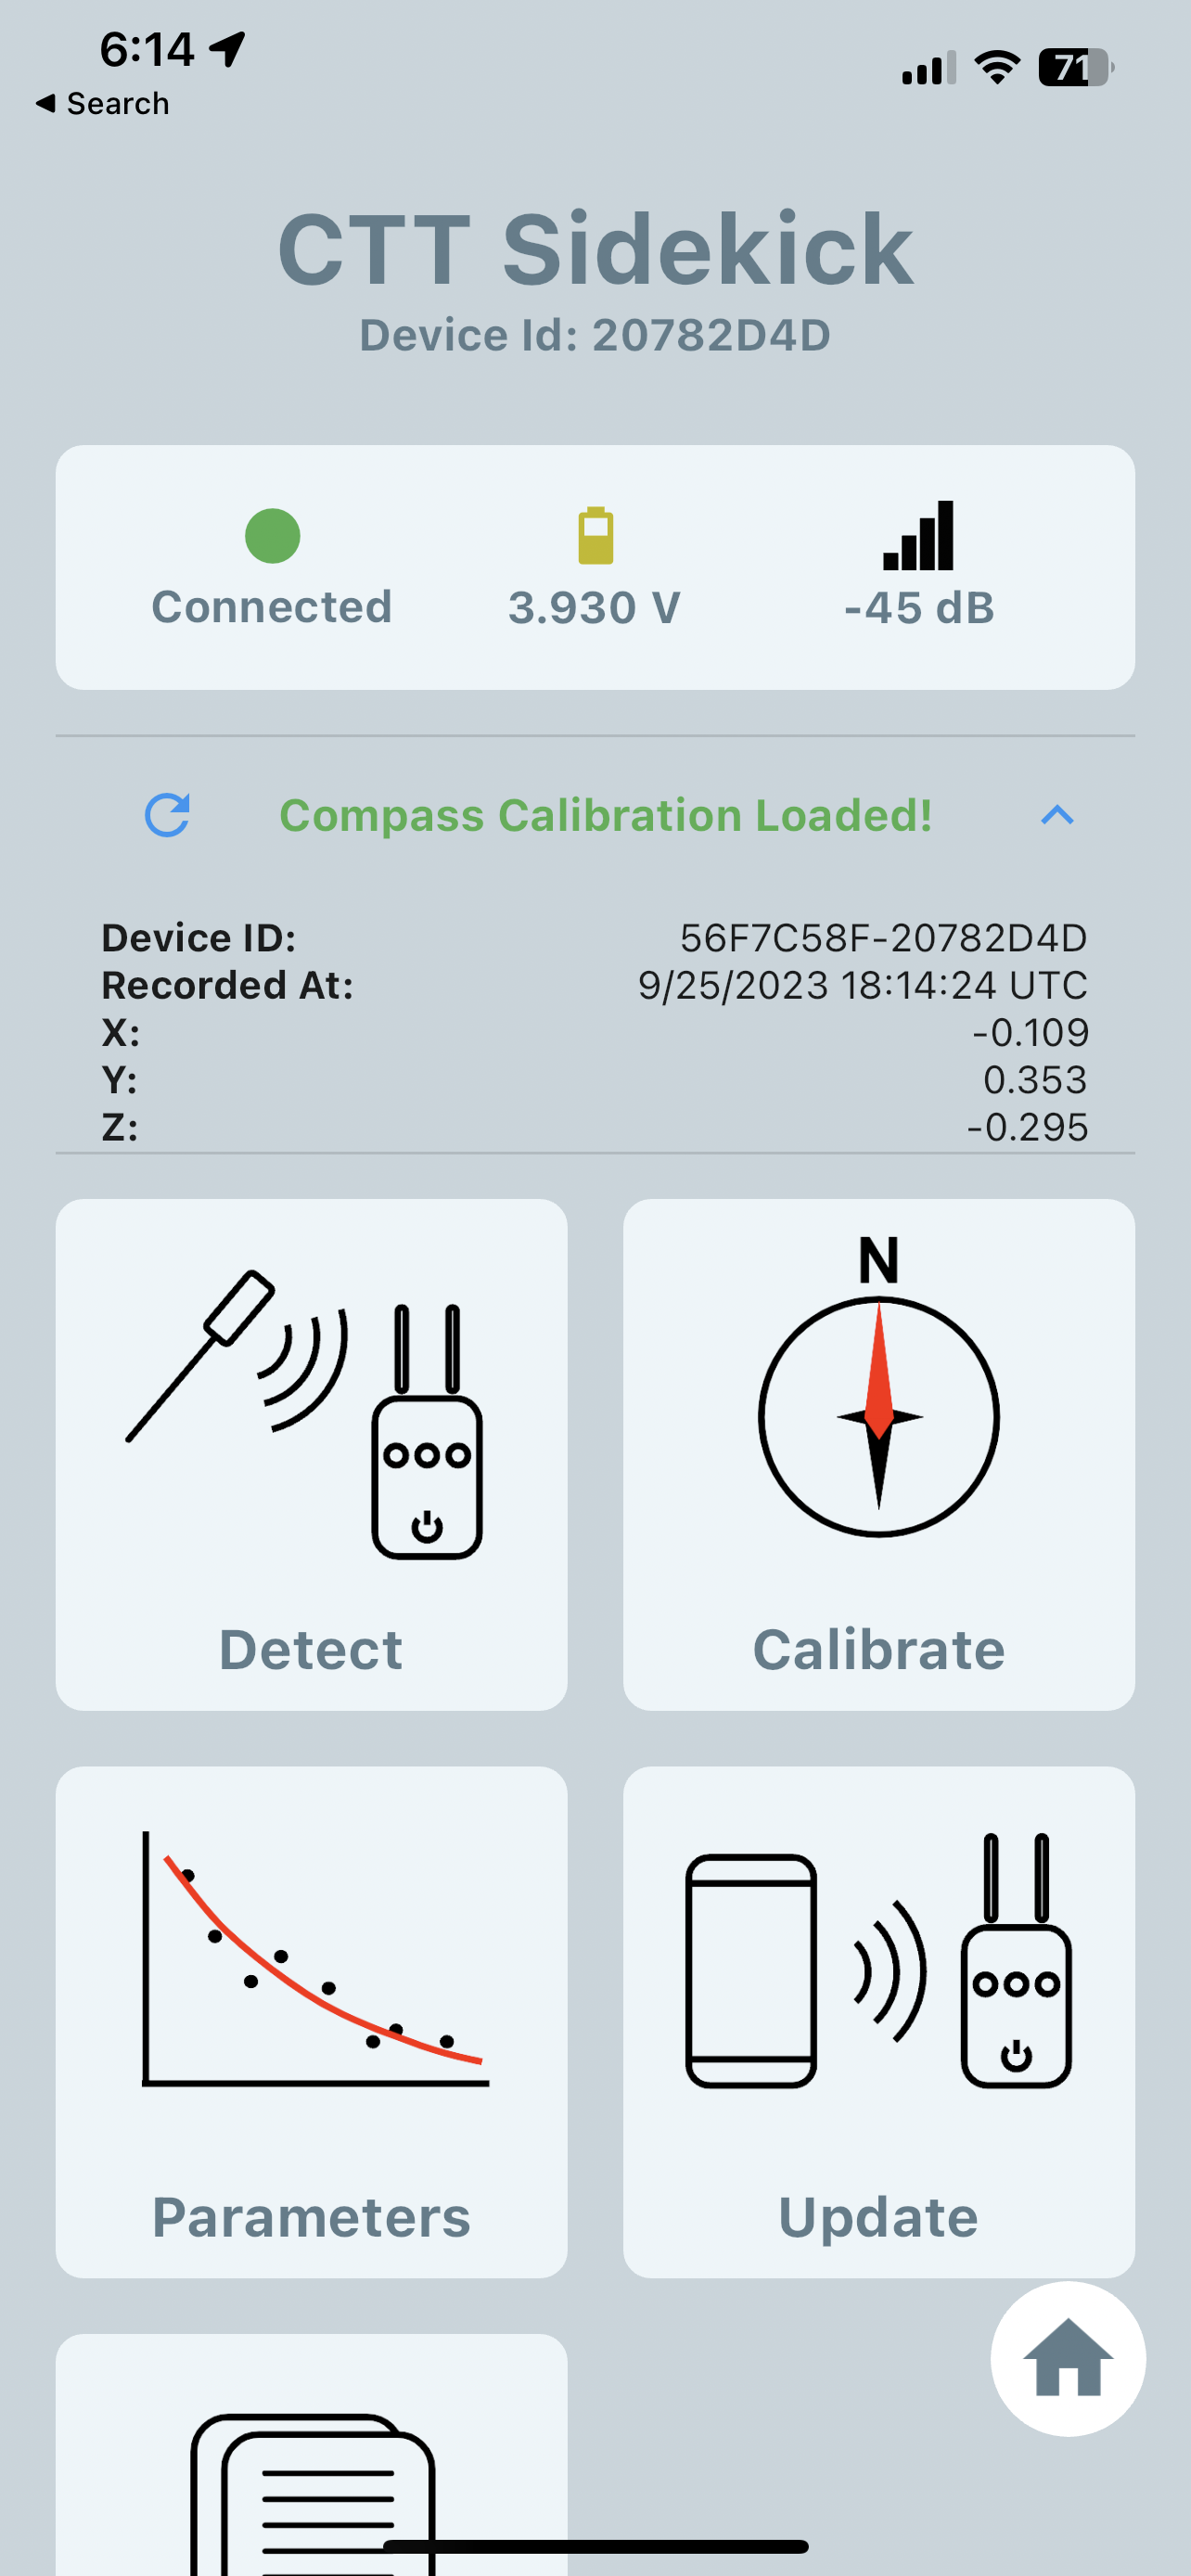
\includegraphics[width=0.25\textwidth,height=\textheight]{./images/sidekick_calibratedCompass.PNG}

\hypertarget{detect-tags}{%
\subsection{Detect Tags}\label{detect-tags}}

The main feature of the CTT Sidekick is its ability to detect radio
tags. From the CTT Sidekick Main Hub screen select the ``Detect'\,'
launch tile to navigate to the Tag List screen.

At the very top right of the Detect Tags screen, in the header, are two
small buttons:

\begin{itemize}
\item
  \textbf{\texttt{X}} - This button clears the Detection List. You may
  find this useful when you have scanned an area where you had multiple
  detections, but then move to a new area, just to see only the tags
  currently within range of your Sidekick.
\item
  \textbf{\texttt{Location\ Icon}} - This button toggles whether you
  enable Location Services, which are required for localizing tags in
  map view, as well as for other features. You can turn this off to save
  battery life when you're not actively tracking tags.
\end{itemize}

Also at the top of the Tag List screen there are three larger buttons:

\begin{itemize}
\item
  \textbf{\texttt{2.4GHz}} - This button toggles the 2.4GHz radio
  receiver on and off. When the radio is on the icon and text will be
  green when it is off the icon and text will be grey.
\item
  \textbf{\texttt{434MHz}} - This button toggles the 434MHz radio
  receiver on and off. When the radio is on the icon and text will be
  green when it is off the icon and text will be grey.
\item
  \textbf{\texttt{Record/Stop}} - This button starts and stops the
  recording of tag detections. When recording is in progress all tag
  detections will be written to a csv file along with the current
  location recorded from your mobile device's GPS receiver.
\end{itemize}

Just below the row of buttons you'll find the a row with actions for
sorting and filtering the tag list:

\begin{itemize}
\tightlist
\item
  \textbf{\texttt{Tag\ List\ Sort\ Options}} - Tapping this button will
  display a list of options for sorting the tag list.
\end{itemize}

\begin{figure}
\hypertarget{id}{%
\centering
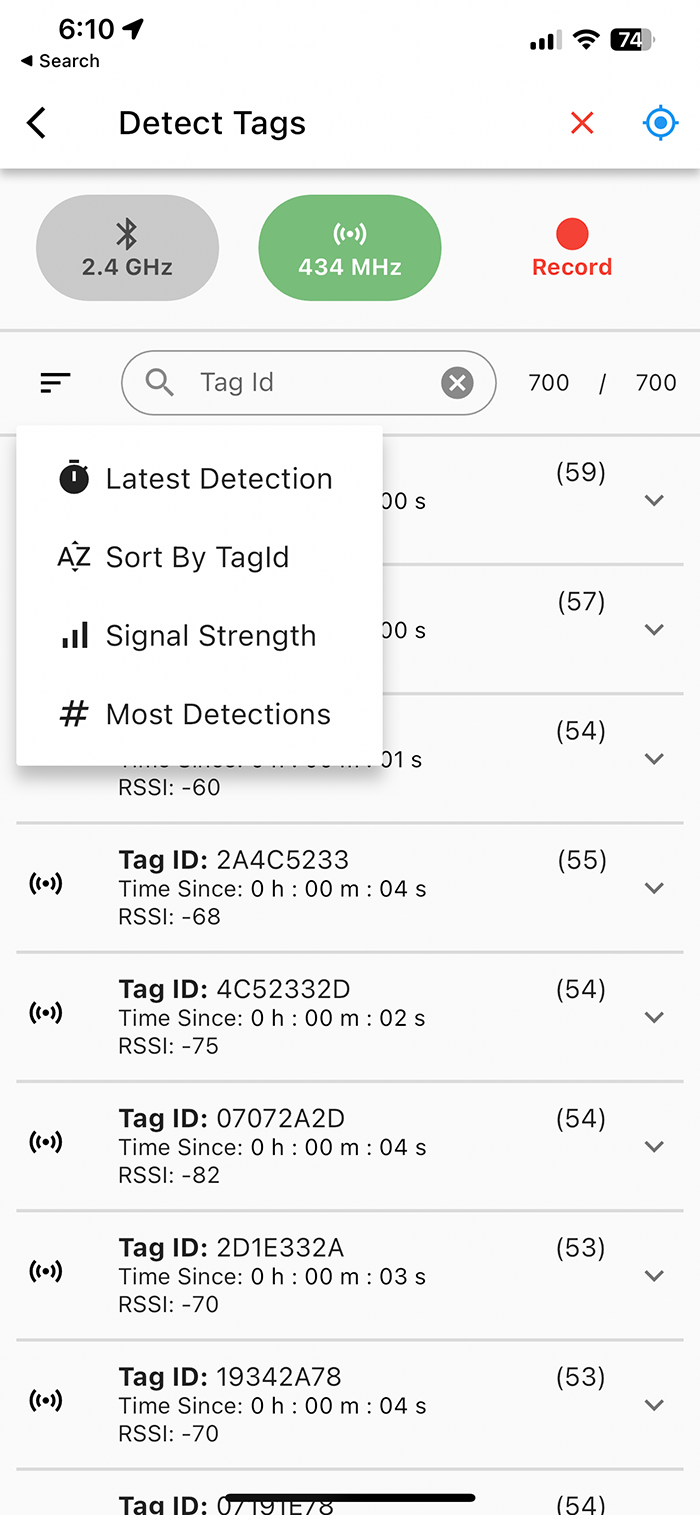
\includegraphics[width=0.25\textwidth,height=\textheight]{./images/ sidekick_sort.PNG}
\caption{Tag Sort Options}\label{id}
}
\end{figure}

\begin{itemize}
\tightlist
\item
  \textbf{\texttt{Tag\ ID\ Search}} - Use this text box to search the
  tag list by tag Id. You can search by partial tag Id. Search is not
  case-sensitive.
\end{itemize}

\begin{figure}
\hypertarget{id}{%
\centering
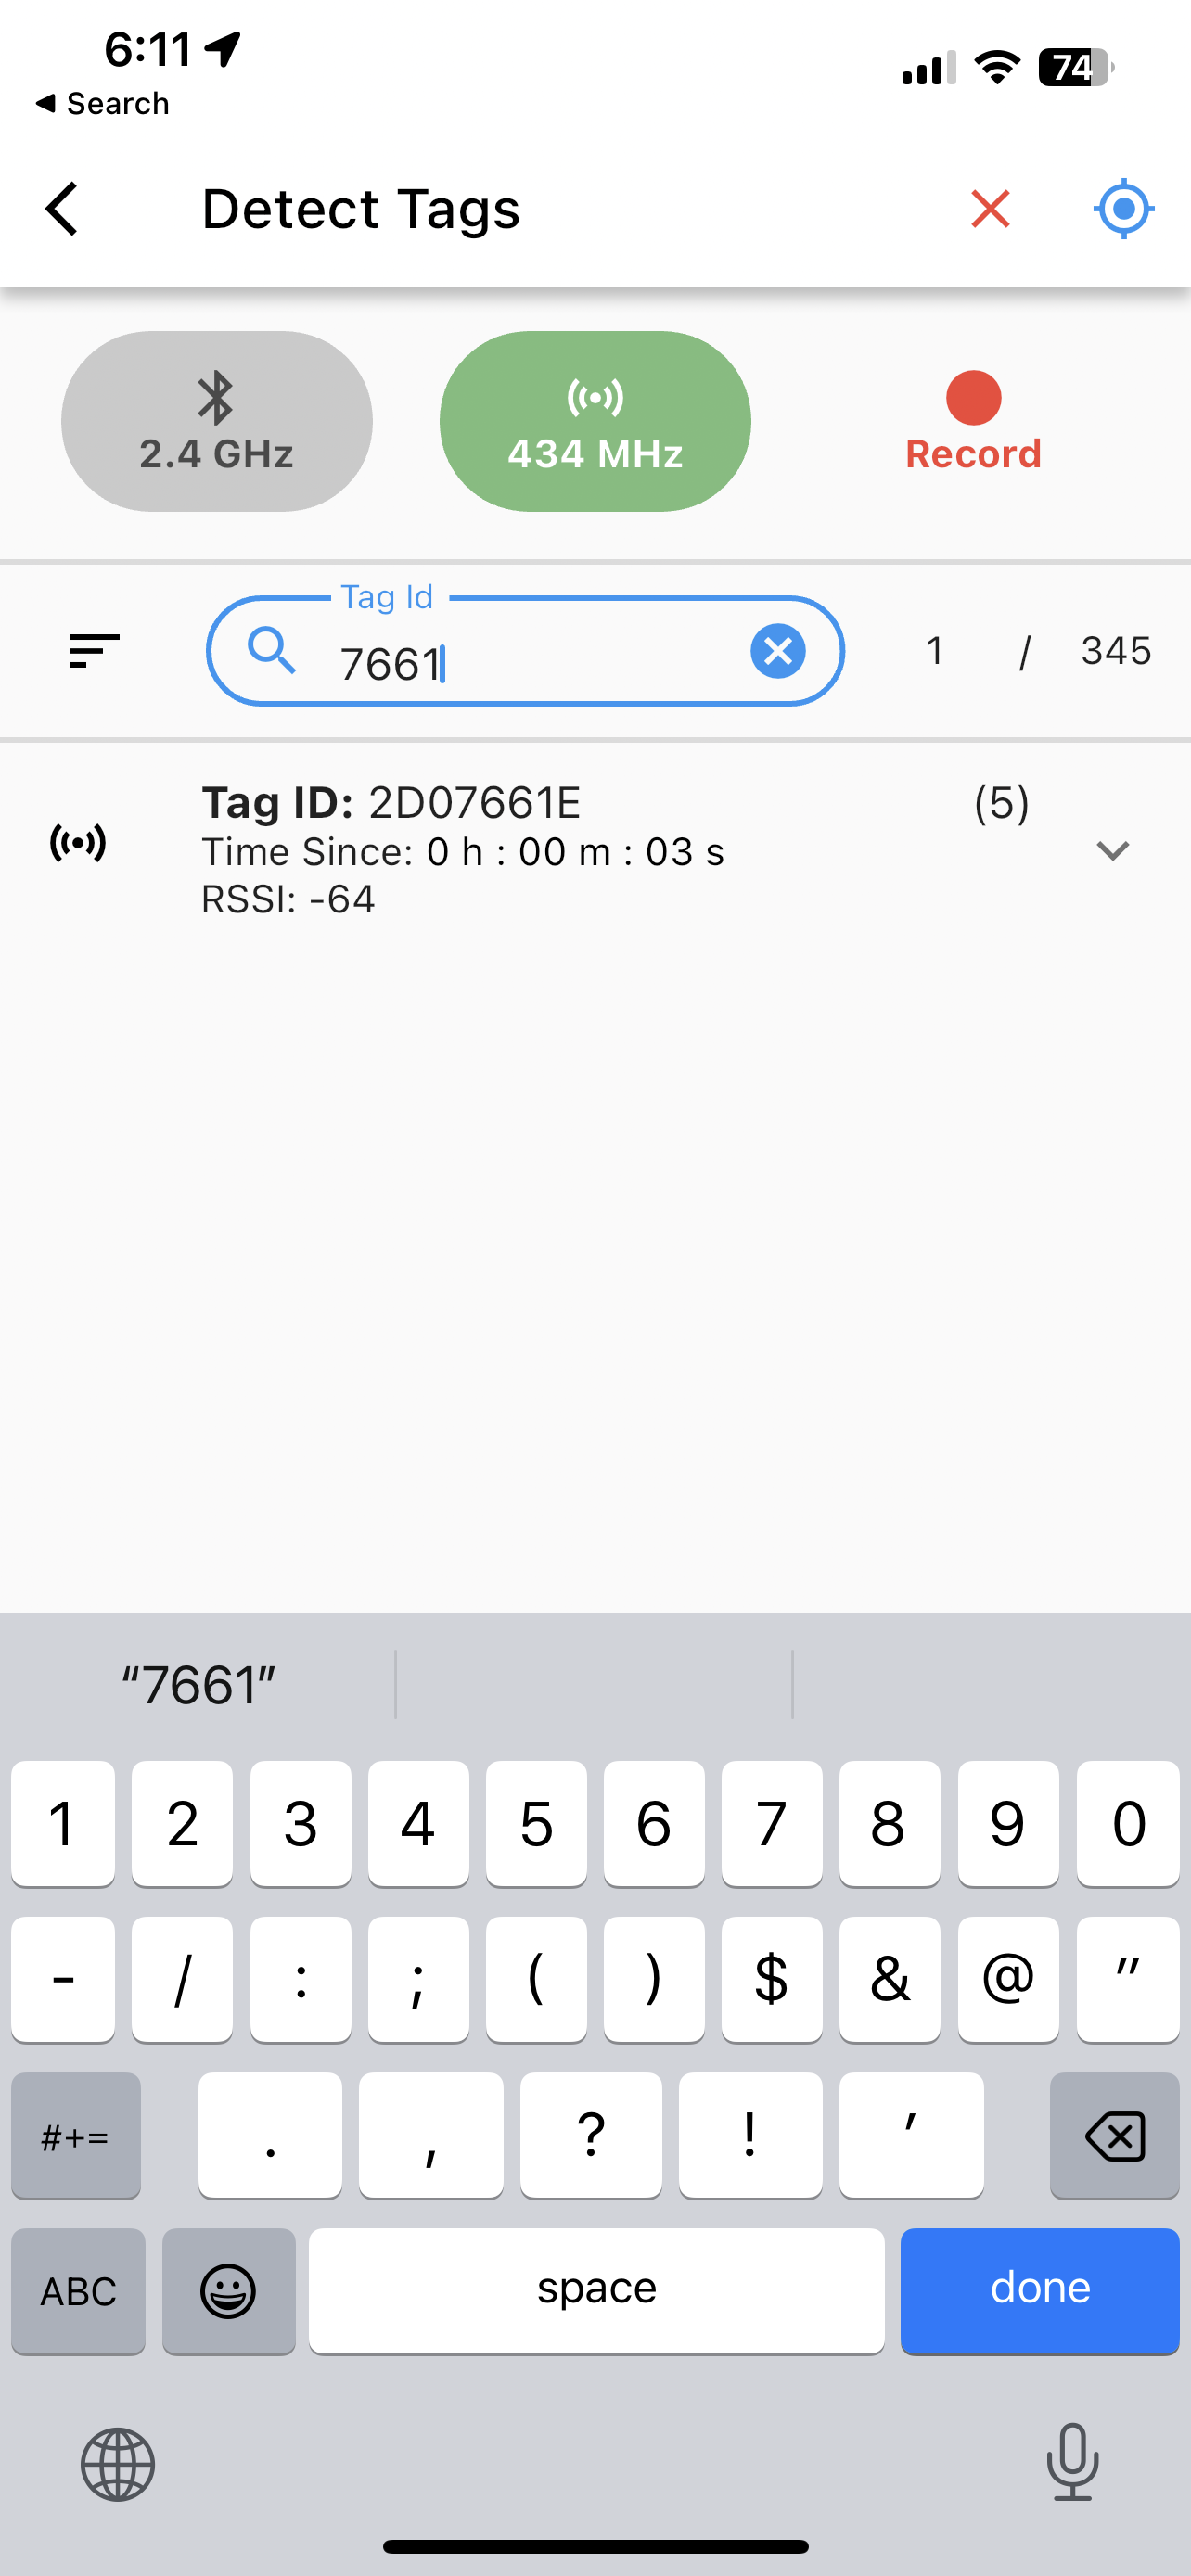
\includegraphics[width=0.25\textwidth,height=\textheight]{./images/sidekick_searchTagID.PNG}
\caption{Tag ID Search}\label{id}
}
\end{figure}

\begin{itemize}
\tightlist
\item
  \textbf{\texttt{Tag\ Count}} - You will see two numbers ``X / Y'\,'.
  Where Y is total number of tags detected since starting the app and X
  is number currently being displayed due to list filtering such as
  searching for a tag Id.
\end{itemize}

Clicking on an individual tag opens up the chart for that tag, as well
as several more options:

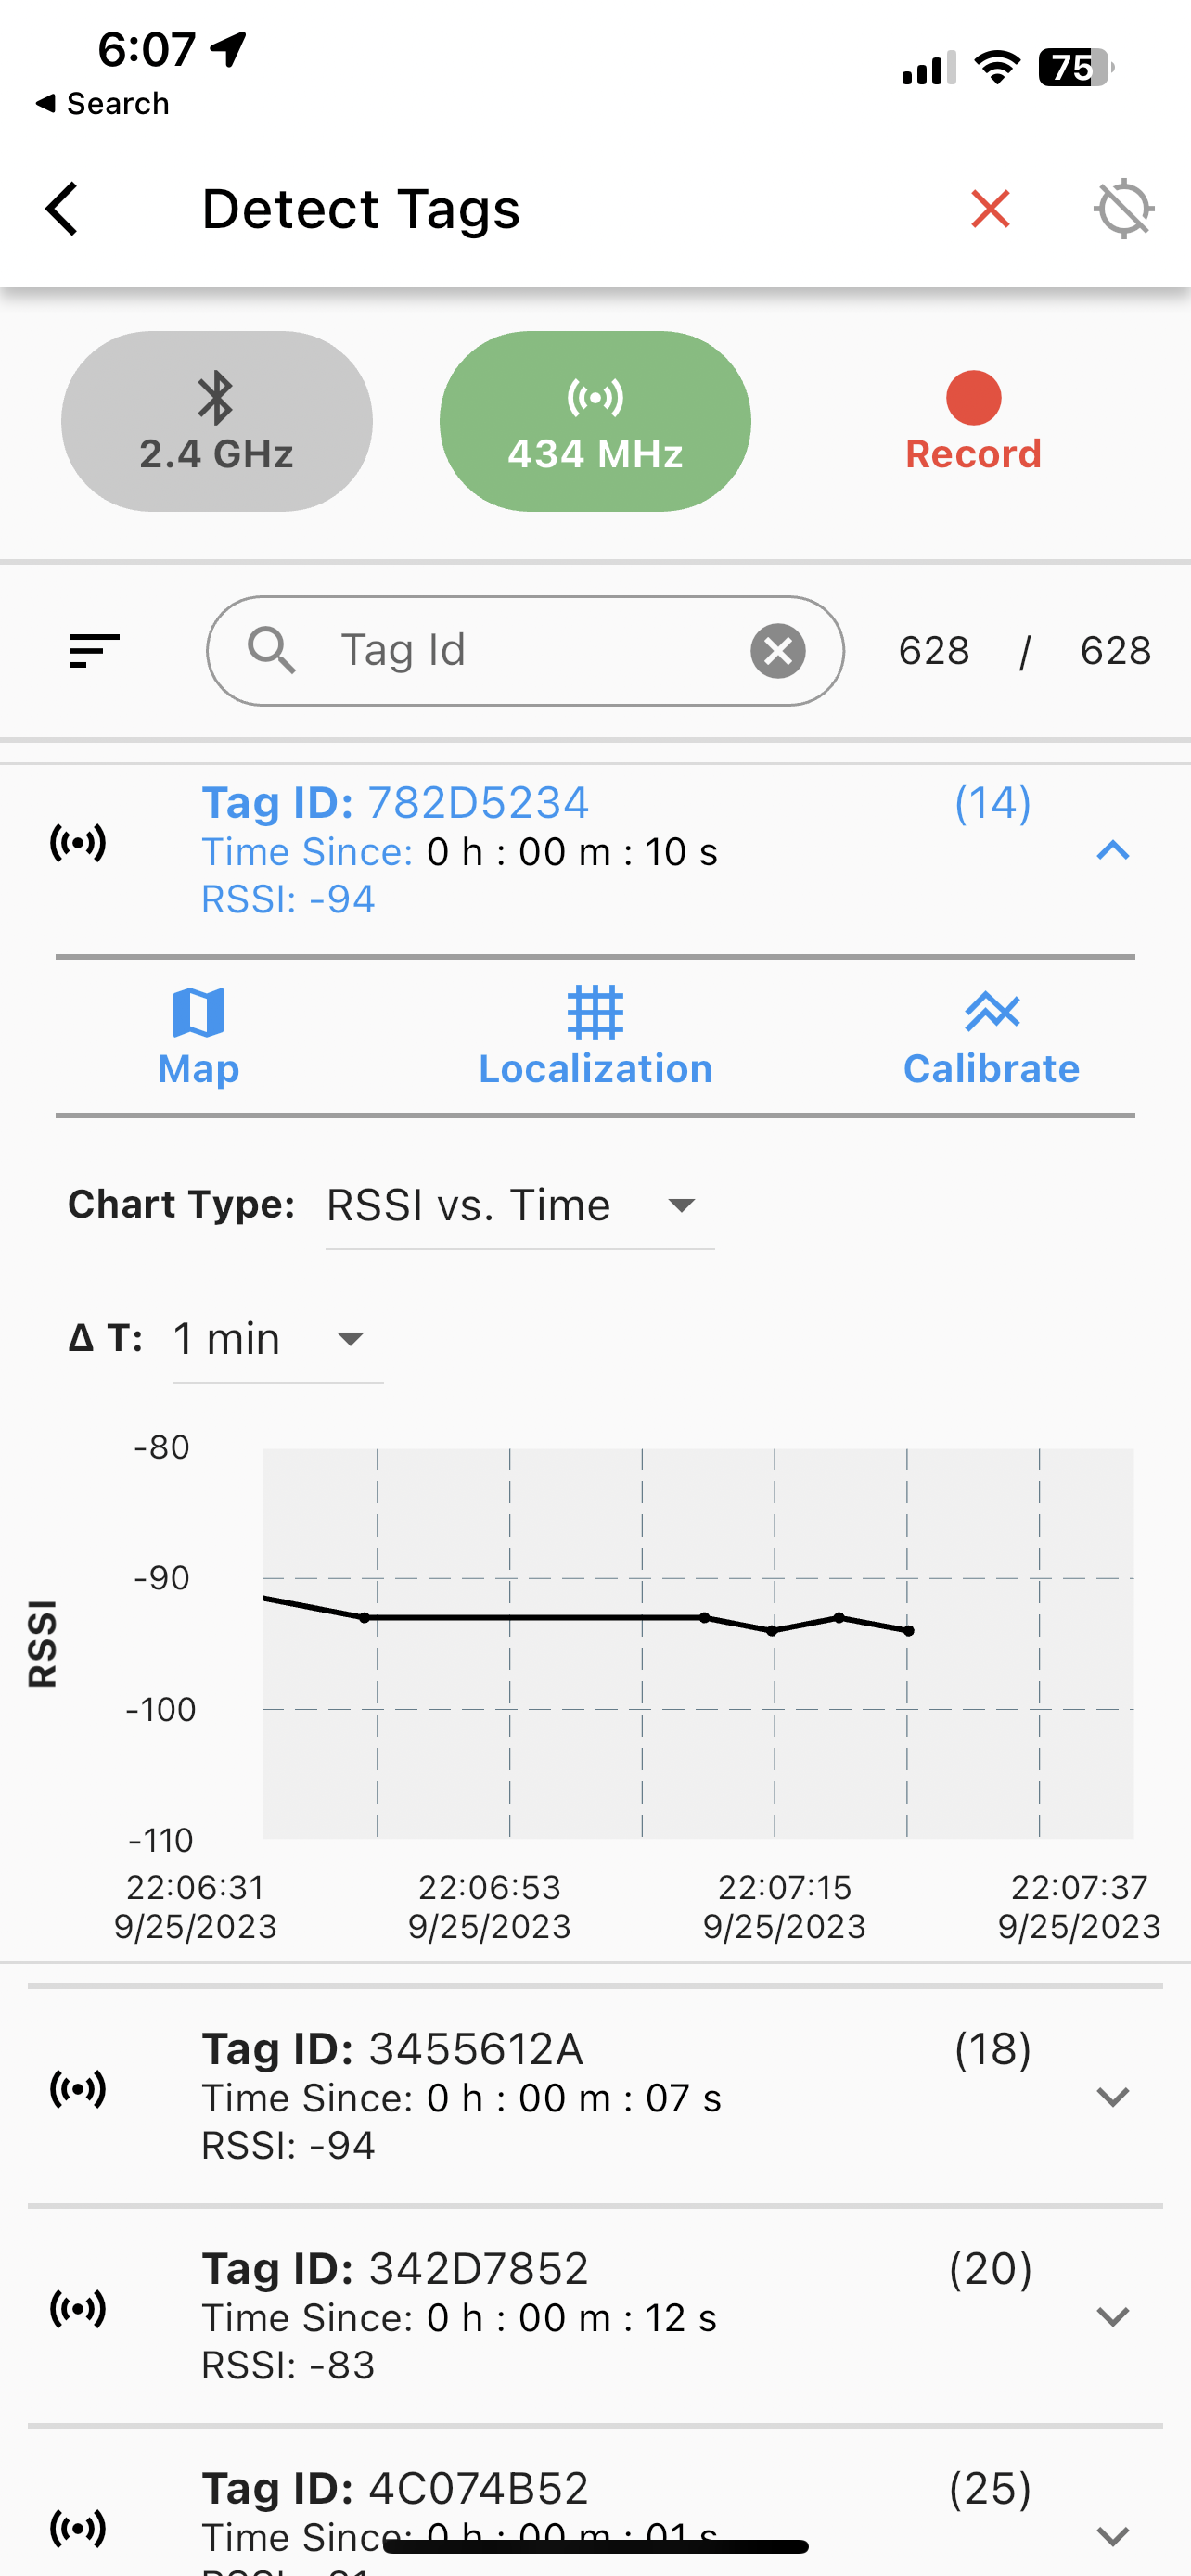
\includegraphics[width=0.25\textwidth,height=\textheight]{./images/sidekick_DetectTag.PNG}

\textbf{\texttt{Chart\ Type}}: Options include \texttt{RSSI\ vs.\ Time},
\texttt{RSSI\ Histogram}, \texttt{Solar\ Voltage}, \texttt{Temperature}

\textbf{\texttt{Change\ Over\ Time}}: Options include \texttt{10s},
\texttt{30s}, \texttt{1min}, \texttt{2min}, \texttt{5min}

\textbf{\texttt{Map}}: Opens the \texttt{Map} window

\textbf{\texttt{Localization}}: Opens the \texttt{Localization} window

\textbf{\texttt{Calibrate}}: Opens the \texttt{Calibration} window

\hypertarget{map-view}{%
\subsection{Map View}\label{map-view}}

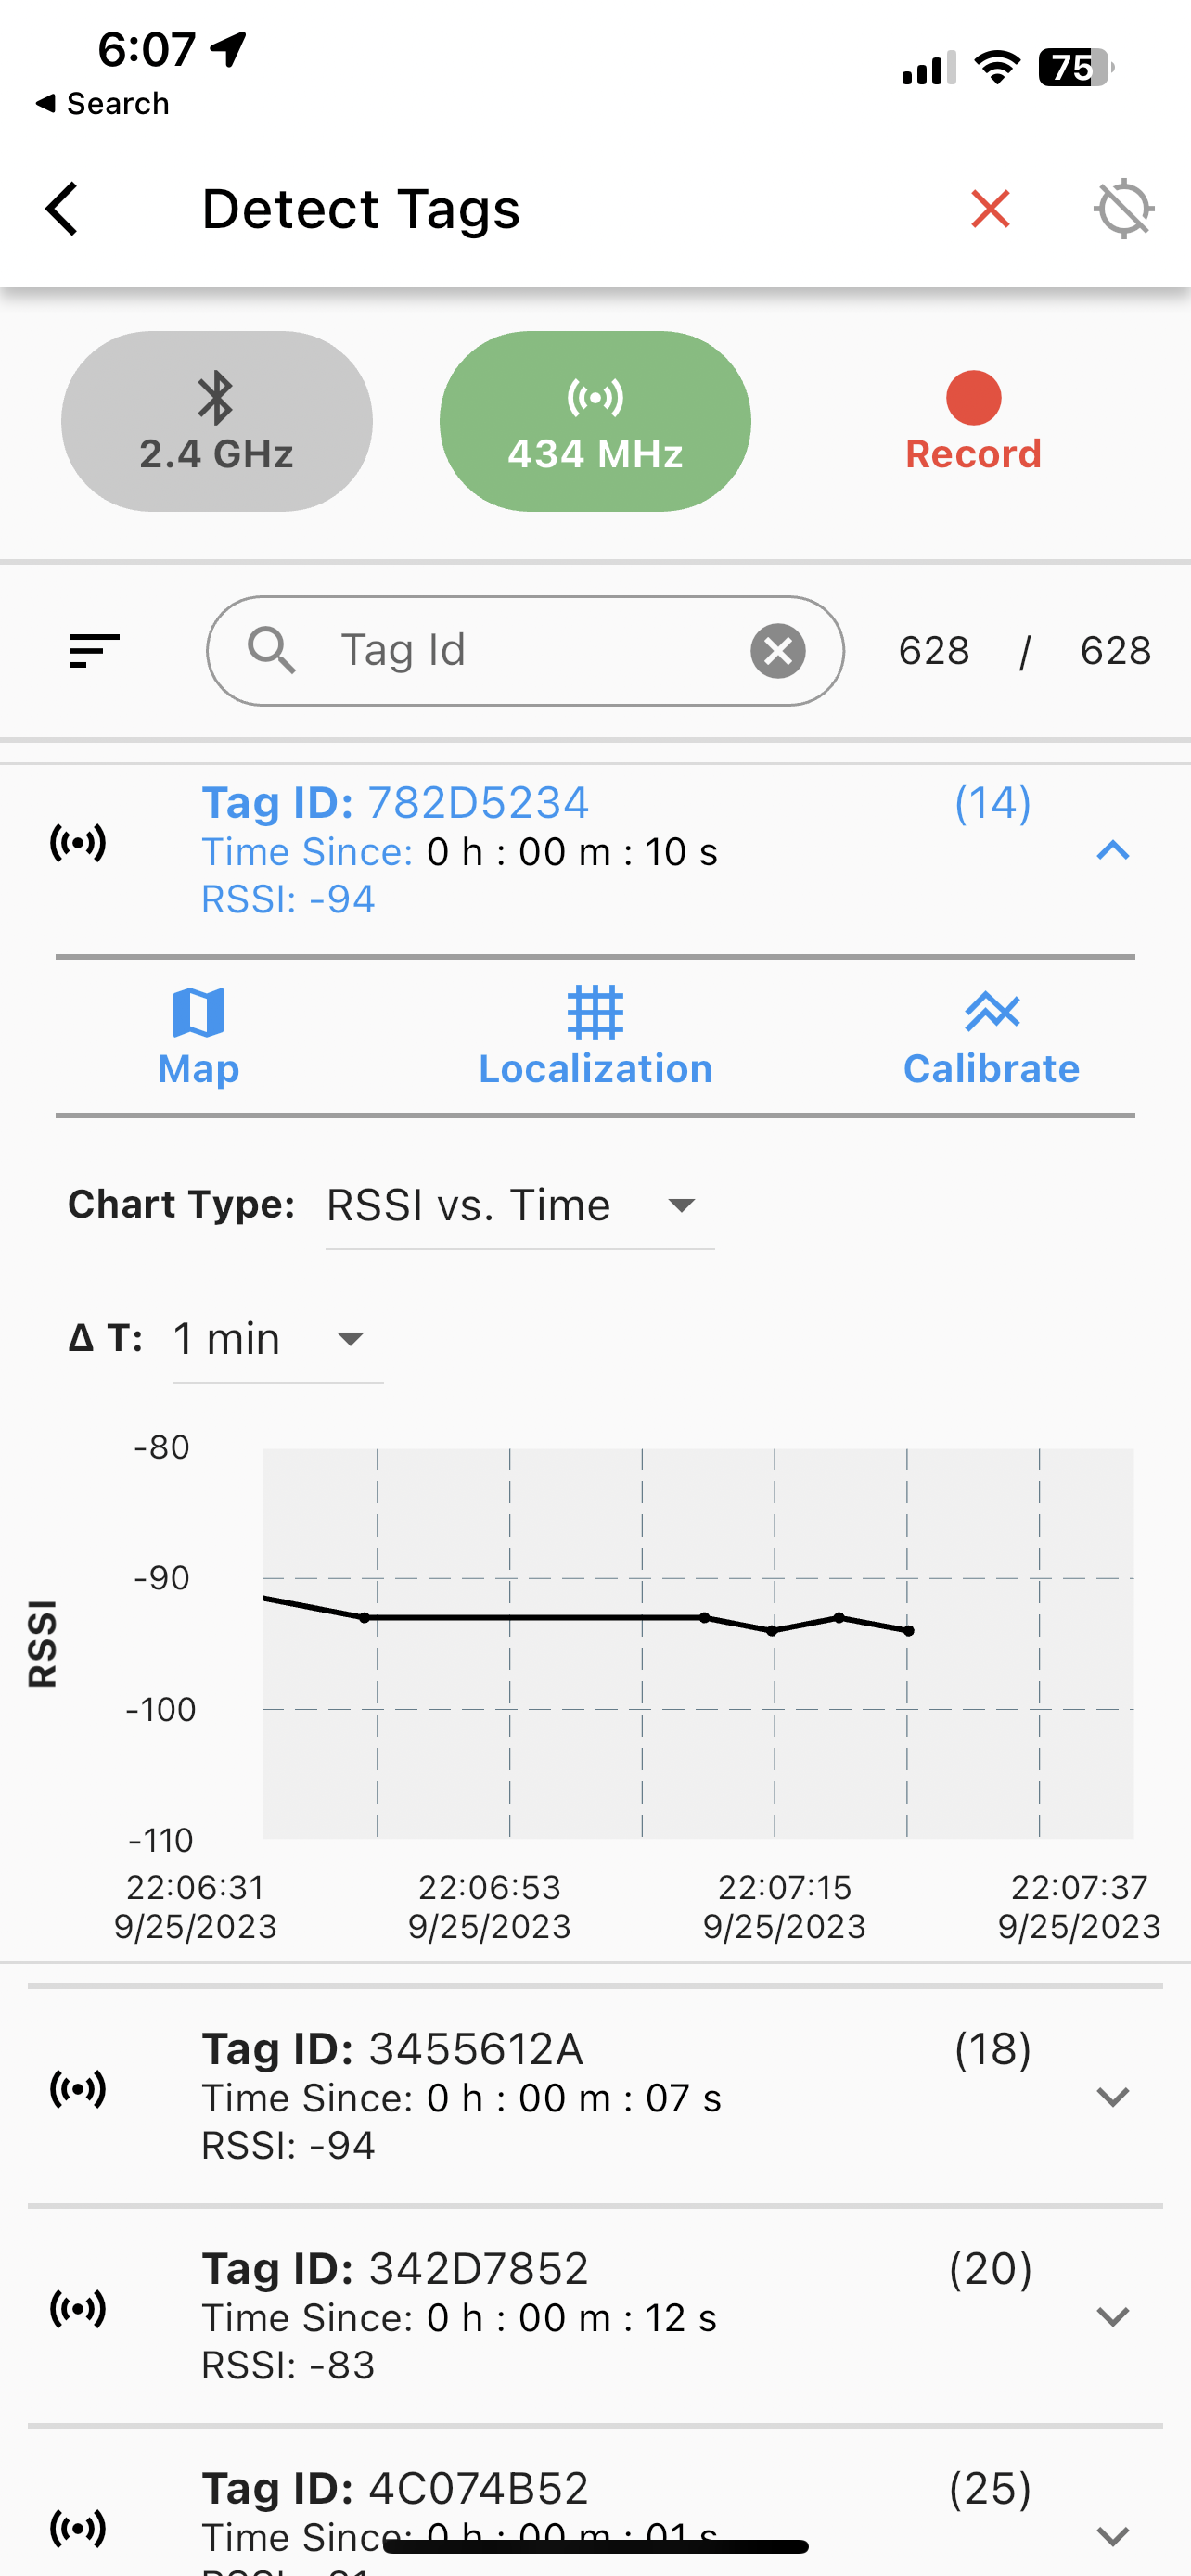
\includegraphics[width=0.25\textwidth,height=\textheight]{./images/sidekick_DetectTag.PNG}
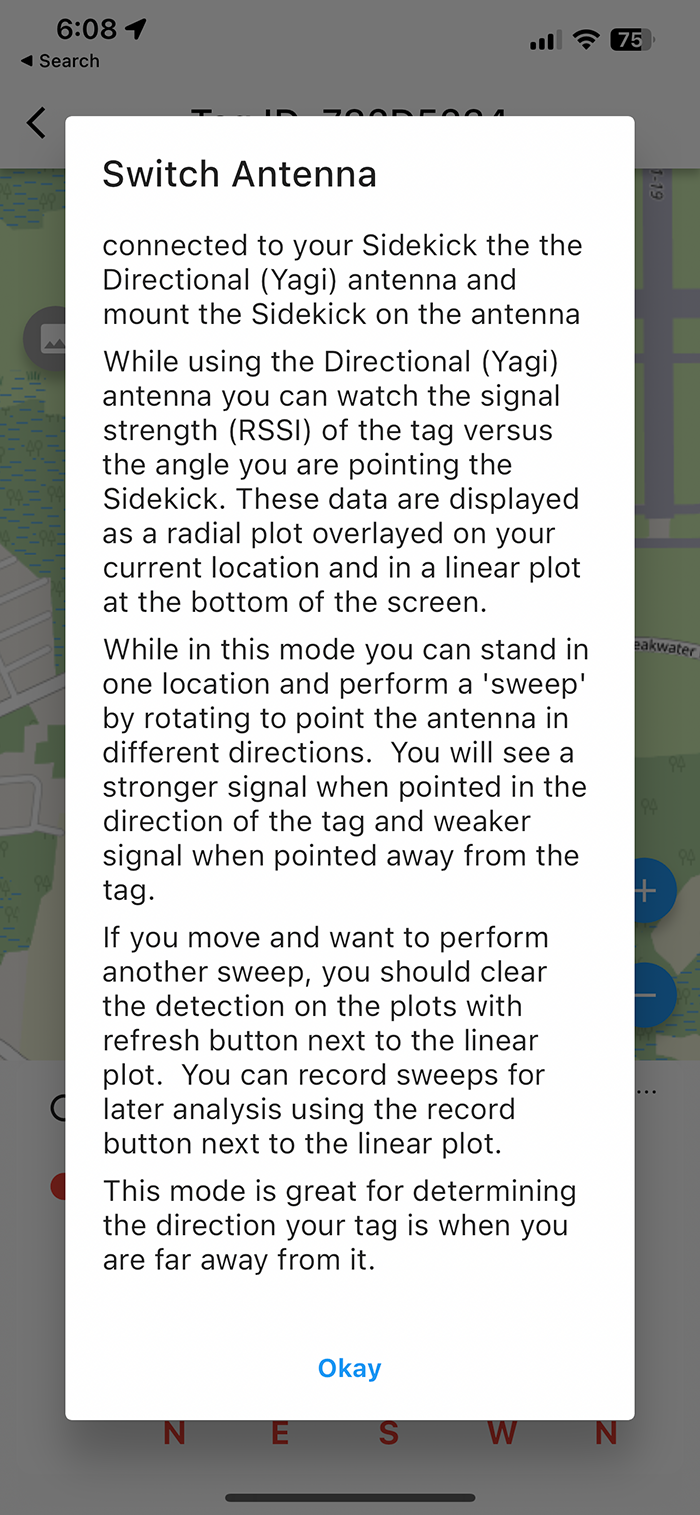
\includegraphics[width=0.25\textwidth,height=\textheight]{./images/sidekickMap_YagiAntTip.PNG}
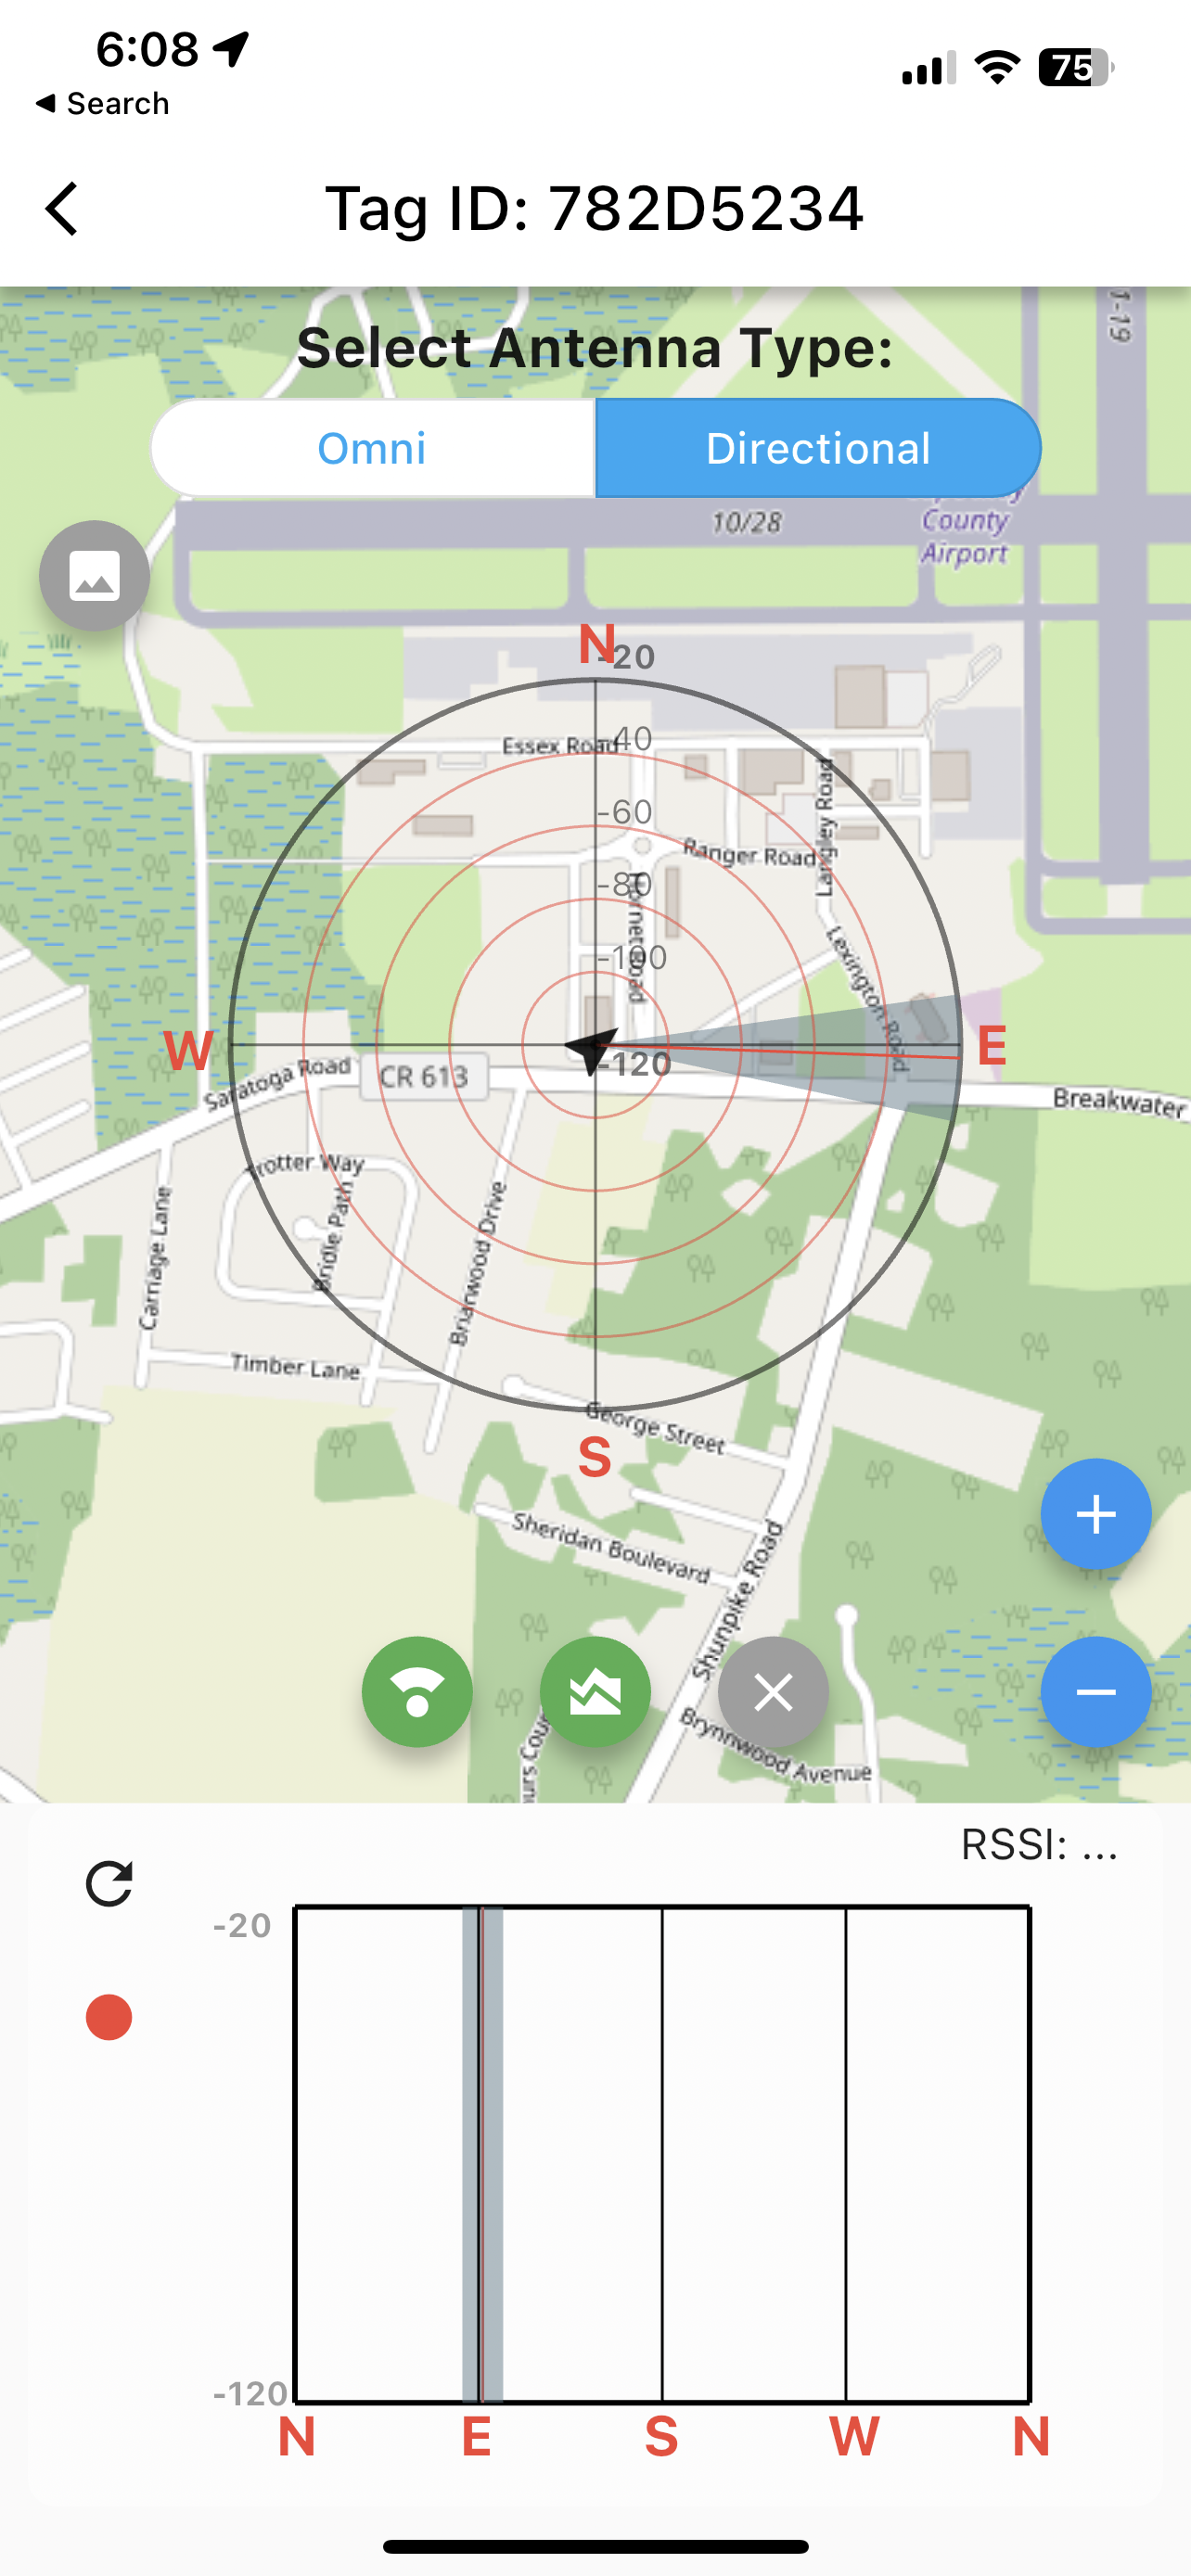
\includegraphics[width=0.25\textwidth,height=\textheight]{./images/sidekickMap_YagiAnt.PNG}
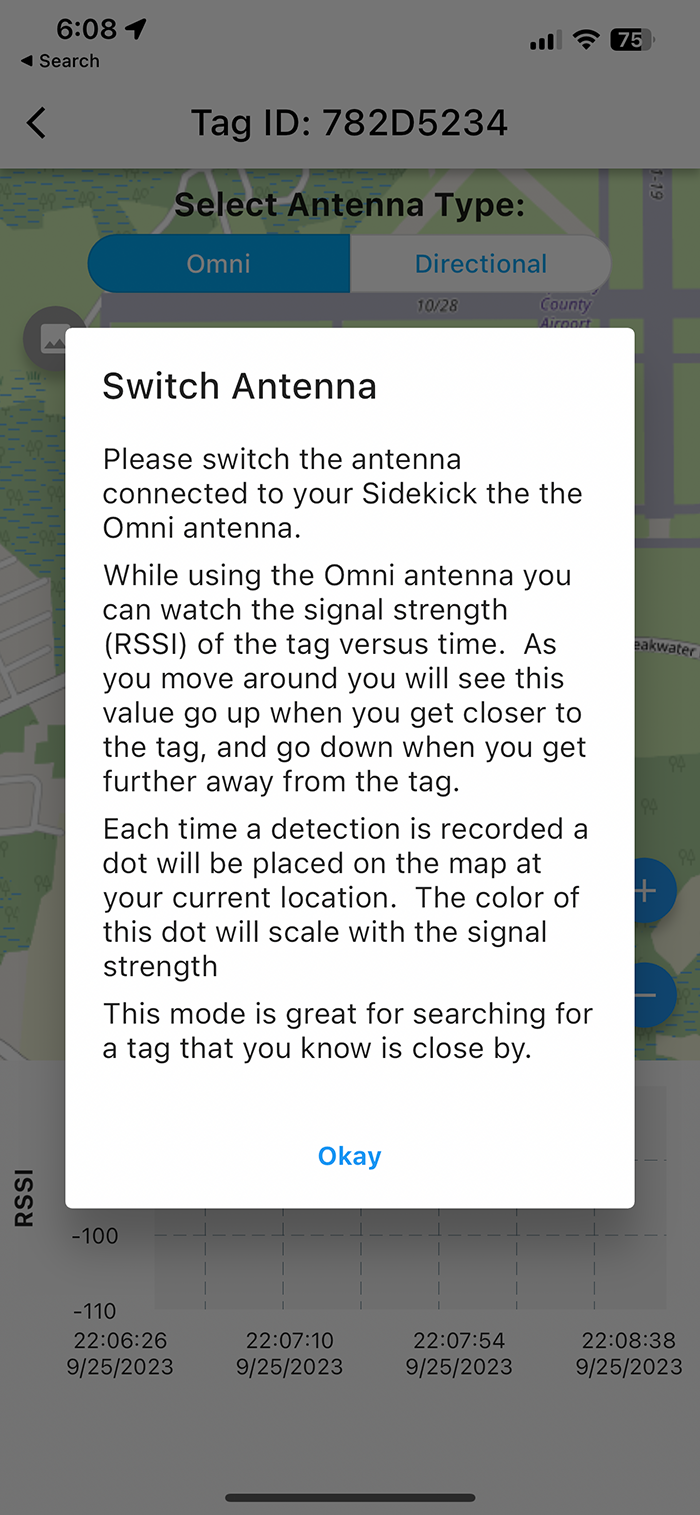
\includegraphics[width=0.25\textwidth,height=\textheight]{./images/sidekickMap_ConnectOmniTip.PNG}
\includegraphics[width=0.25\textwidth,height=\textheight]{./images/sidekickMap_OmniAnt.PNG}
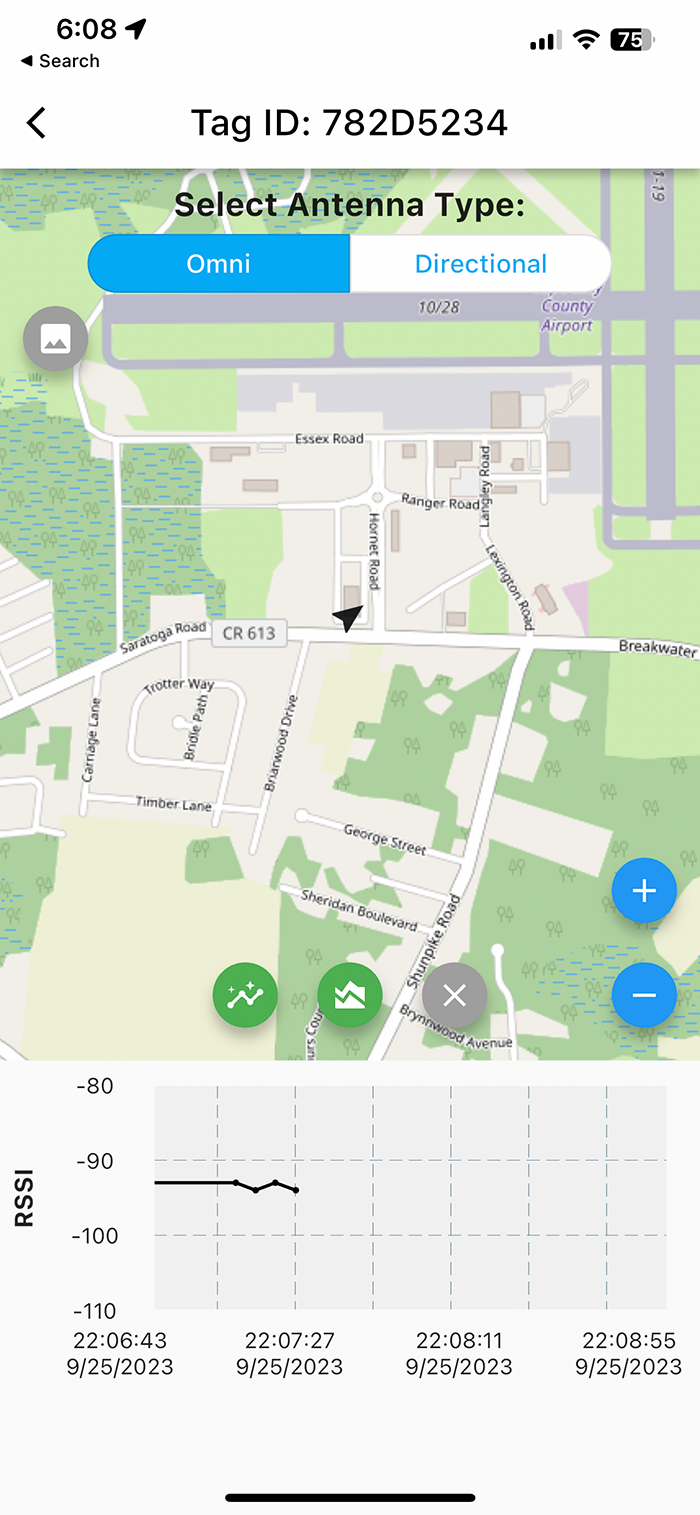
\includegraphics[width=0.25\textwidth,height=\textheight]{./images/sidekickMap_chooseAntenna.PNG}

\hypertarget{localization}{%
\subsection{Localization}\label{localization}}

Please note the warning screen that opens when you click on the
Localization button. While still a Beta feature, Localization provides
you with a powerful tool for finding a stationary tag (great for
relocating a tag that has fallen off of an animal, or on an animal you
suspect has died). In order to use the Localization feature you must
first collect a RSSI vs.~Distance calibration dataset on your tag.
\textbf{This is important, because you must do so before you ever deploy
the tag, so doing so should be part of your pre-deployment checklist.}

Also note that Localization only works with the Omni antenna.

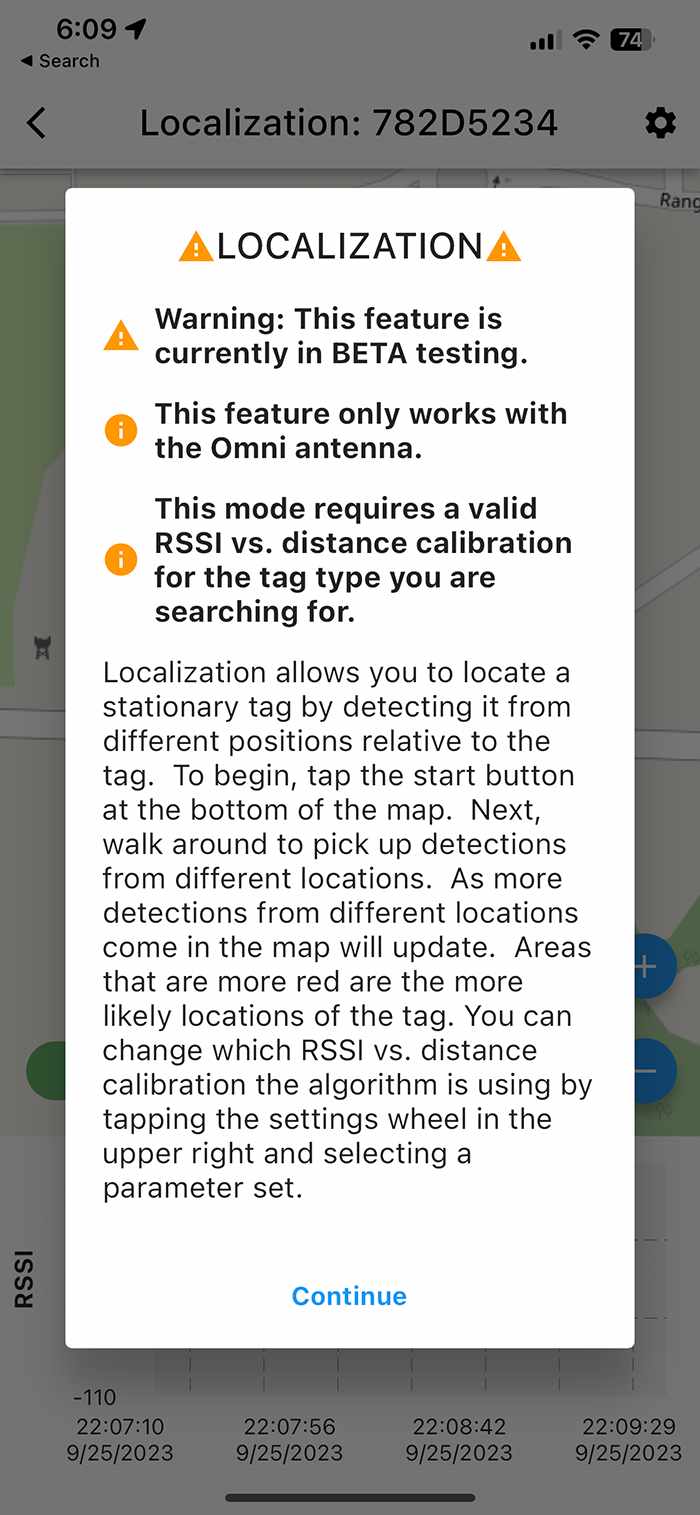
\includegraphics[width=0.25\textwidth,height=\textheight]{./images/sidekick_LocalizationWarn.PNG}

The Localization screen consists of a Heatmap and an RSSI vs.~Time
graph. As more beeps are recorded, the heatmap begins to provide
directionality of your tag. Walking a grid pattern, and keeping your
Sidekick above your head, will allow the algorithm to more accurately
arrive an a solution for your tag's location.

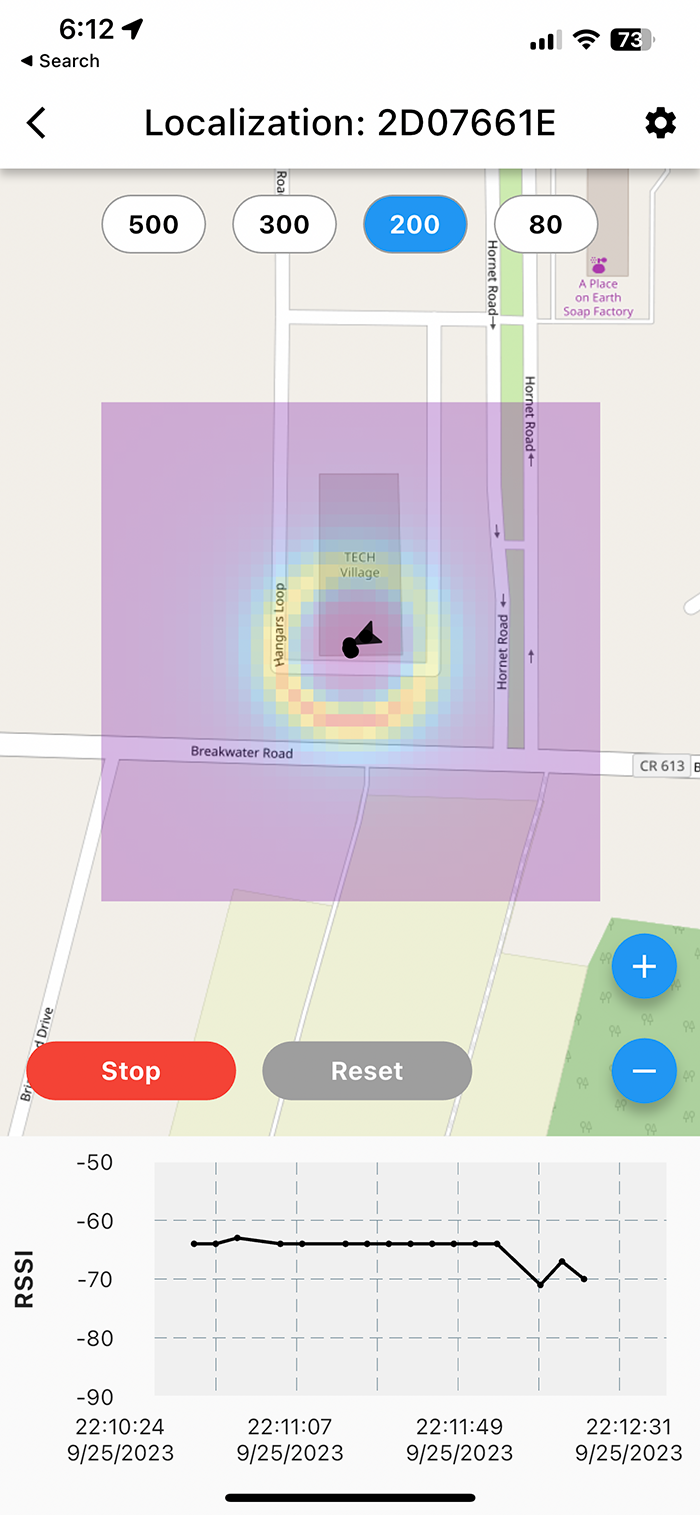
\includegraphics[width=0.25\textwidth,height=\textheight]{./images/sidekick_localization1.PNG}
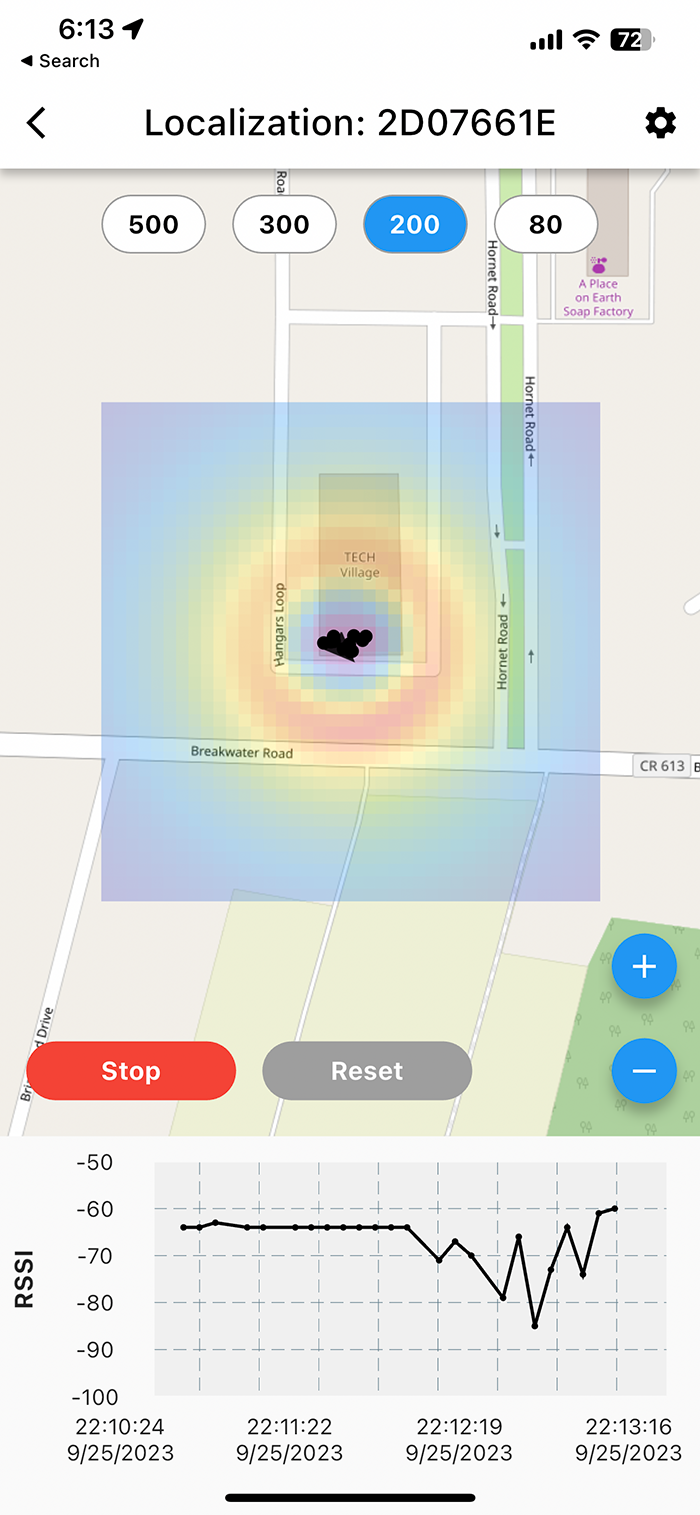
\includegraphics[width=0.25\textwidth,height=\textheight]{./images/sidekick_localizationFinal.PNG}

At the top of the Localization screen are four grid size options,
\texttt{500m}, \texttt{300m}, \texttt{200m}, and \texttt{80m}. As you
get closer to your tag you can increase the resolution of your grid by
selecting a smaller grid size. For tags located farther than 500m away,
consider using the Yagi antenna with the \texttt{Detect} screen until
you are within the grid-size-range, and then switch to the Omni antenna
and use the Localization screen.

\begin{figure}
\hypertarget{id}{%
\centering
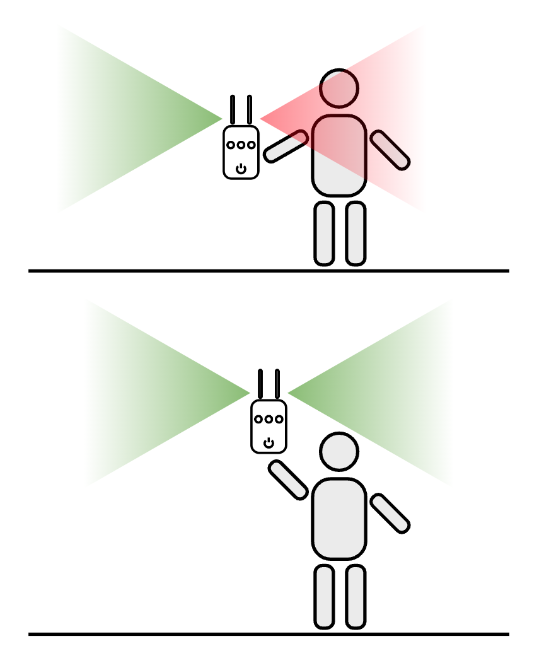
\includegraphics[width=0.5\textwidth,height=\textheight]{./images/localization_orientation.png}
\caption{Example of optimal Sidekick orientation for using
localization}\label{id}
}
\end{figure}

\hypertarget{calibrating-rssi-vs.-distance}{%
\subsection{Calibrating RSSI
vs.~Distance}\label{calibrating-rssi-vs.-distance}}

\begin{figure}
\hypertarget{id}{%
\centering
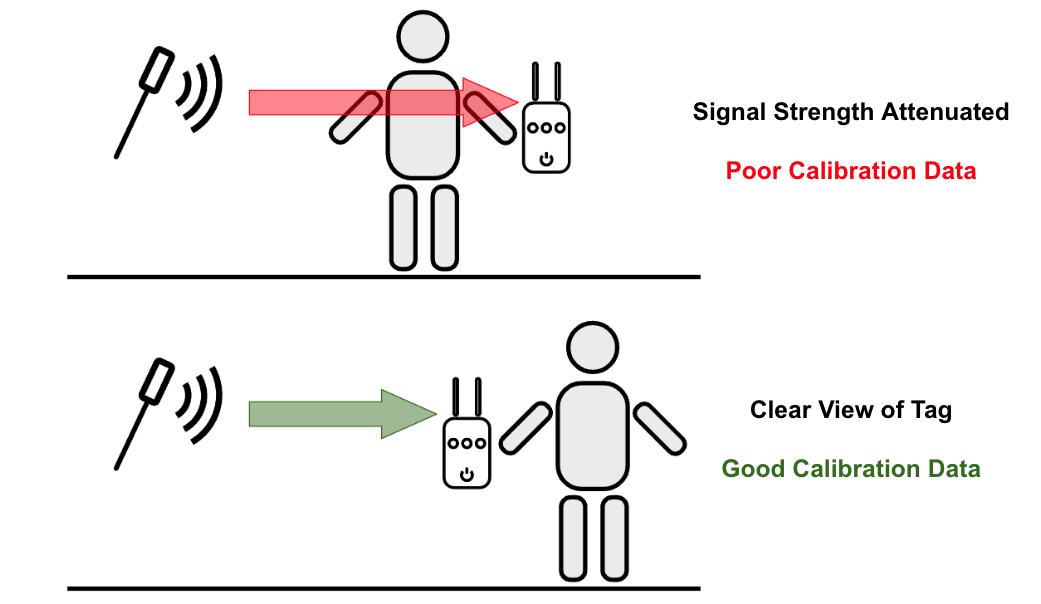
\includegraphics[width=0.5\textwidth,height=\textheight]{./images/calibration_atten_diagram.png}
\caption{Example of tag calibration attenuation}\label{id}
}
\end{figure}

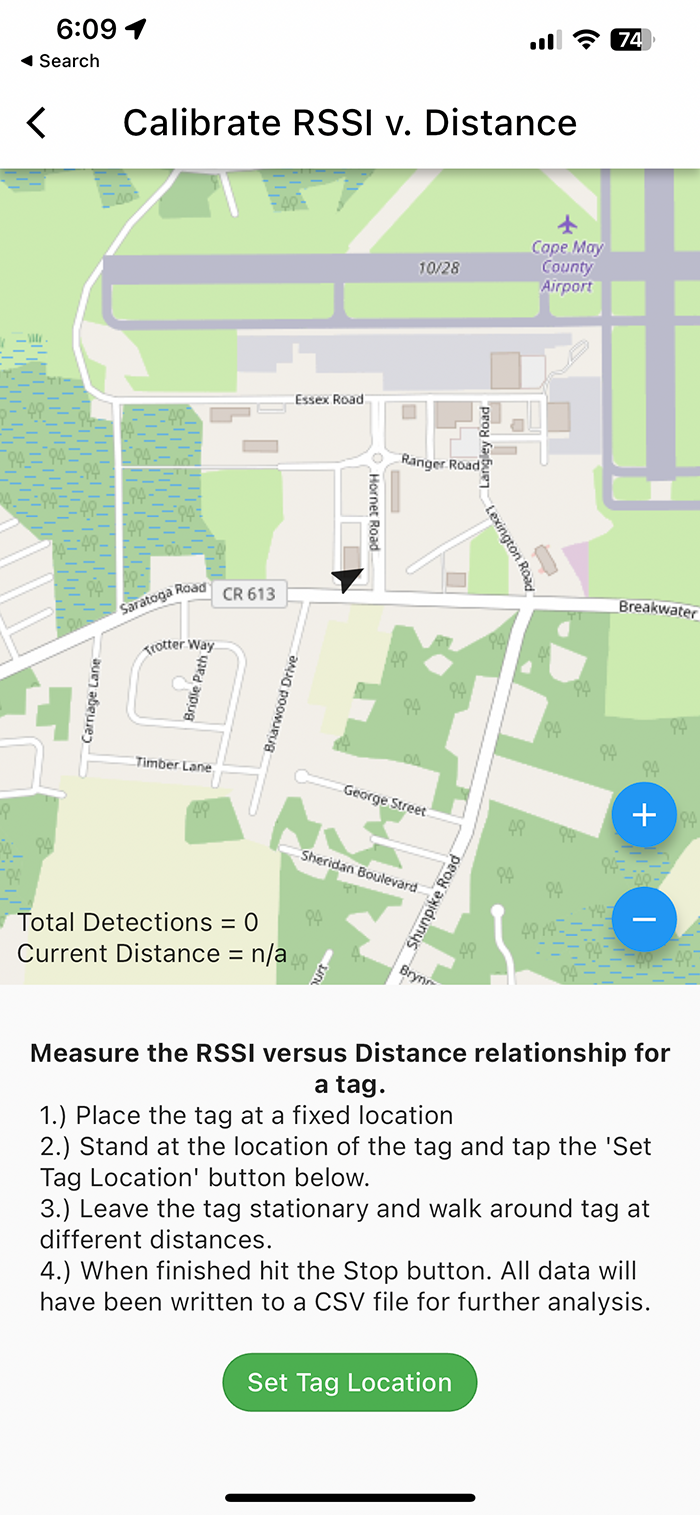
\includegraphics[width=0.25\textwidth,height=\textheight]{./images/sidekick_calibrateTag.PNG}

\hypertarget{rssi-vs.-distance-fit-parameters}{%
\subsection{RSSI vs.~Distance Fit
Parameters}\label{rssi-vs.-distance-fit-parameters}}

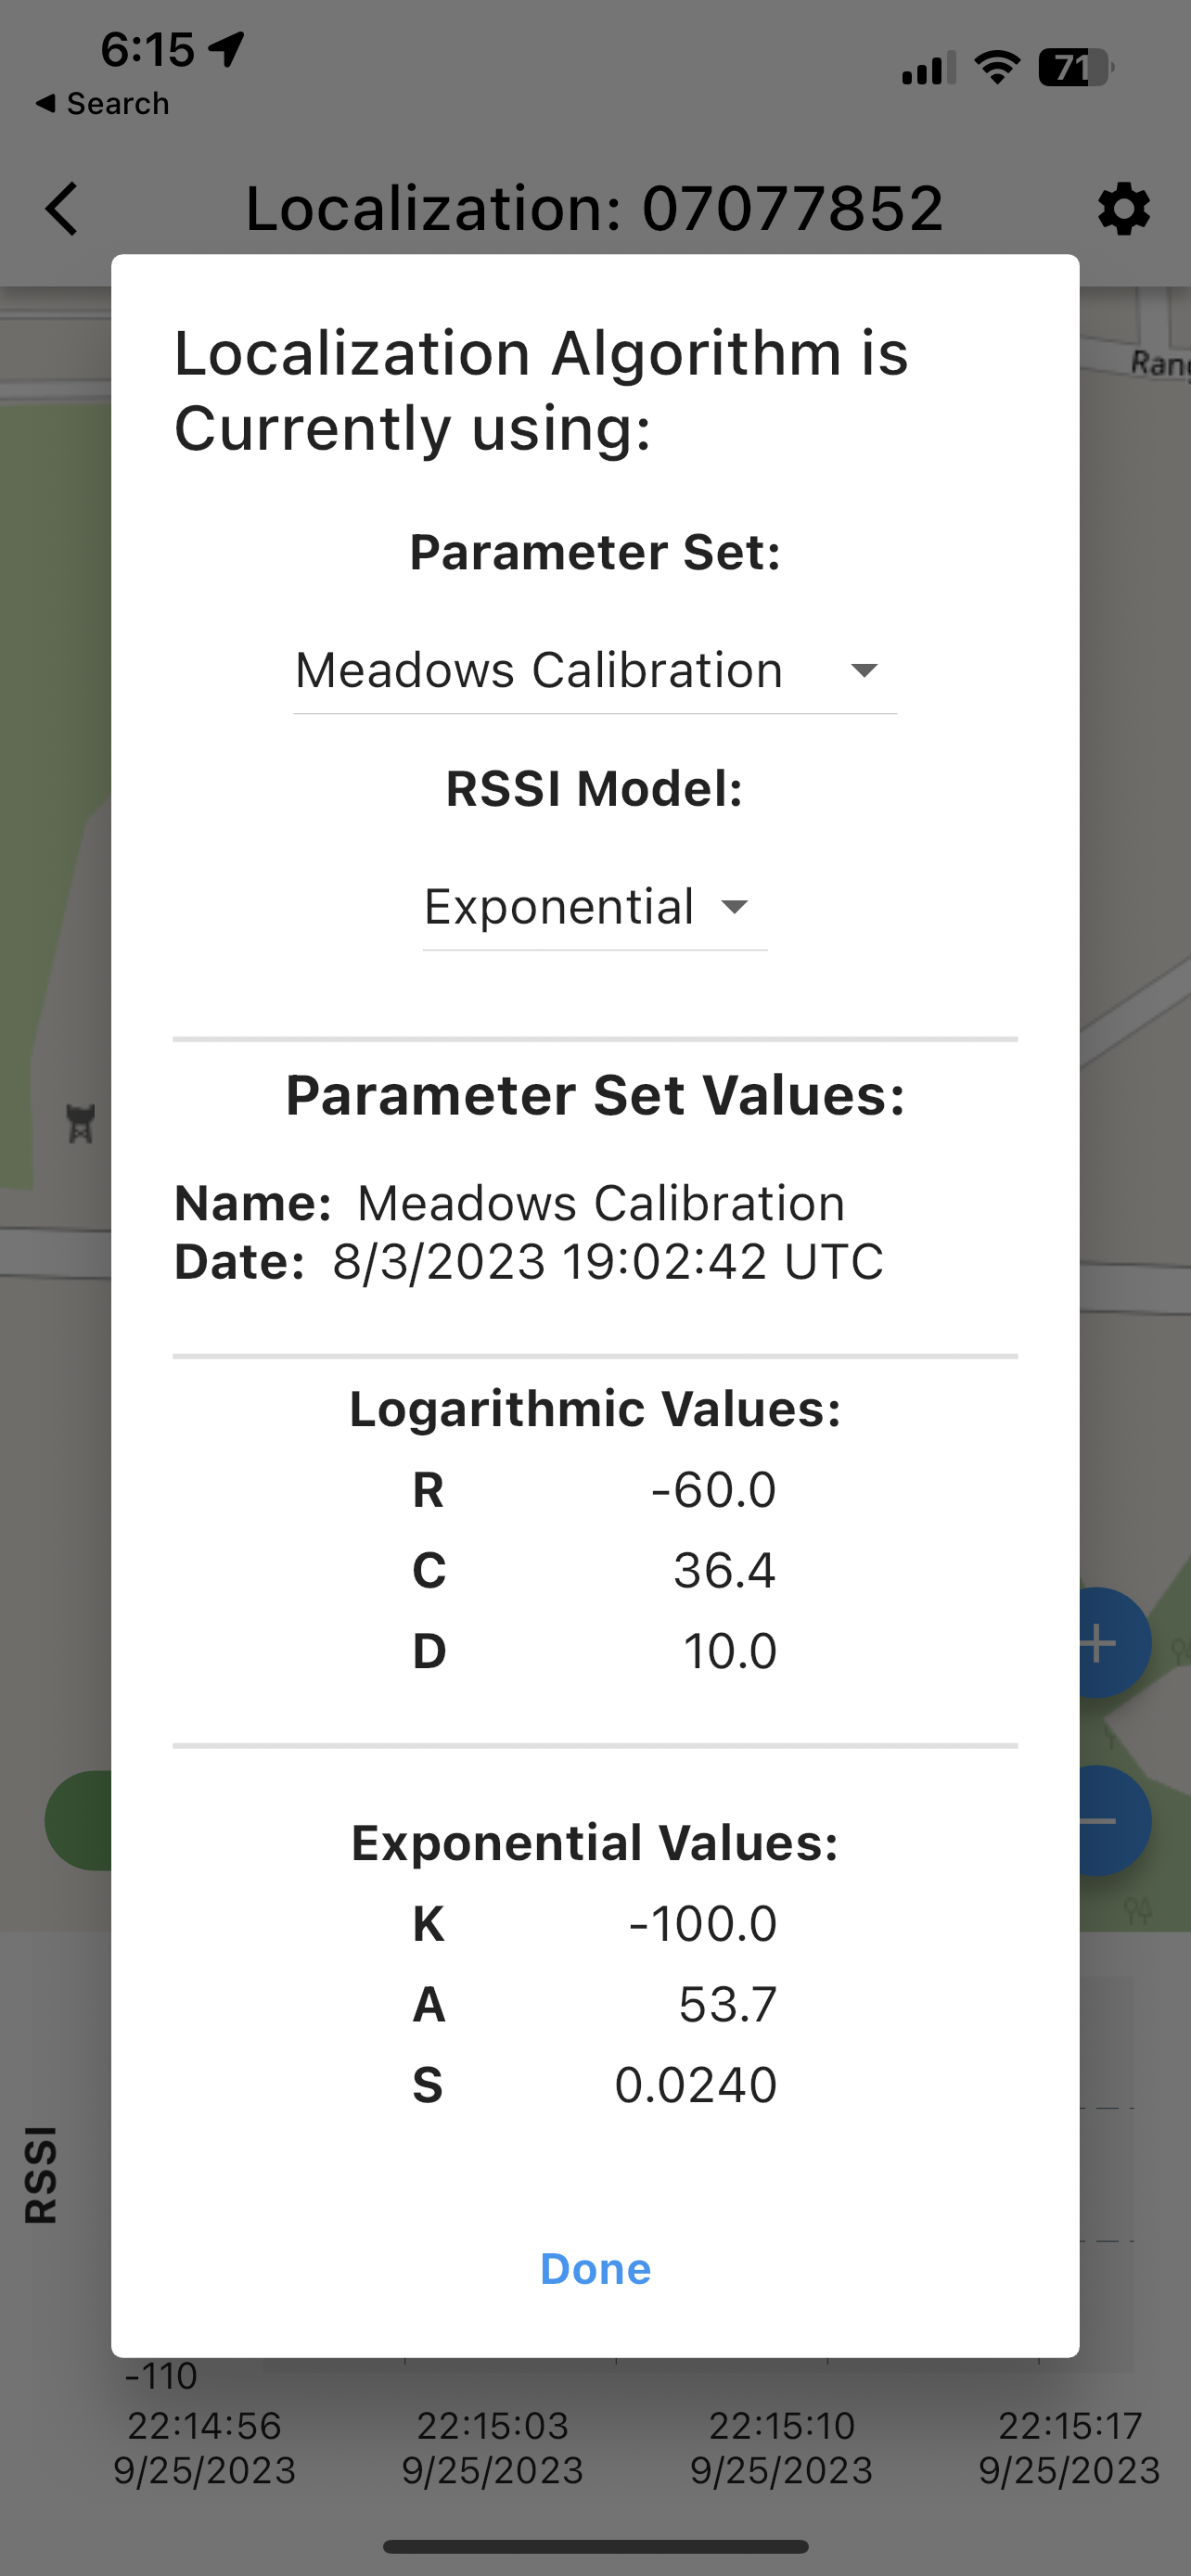
\includegraphics[width=0.25\textwidth,height=\textheight]{./images/sk_localization_choose_alg.PNG}

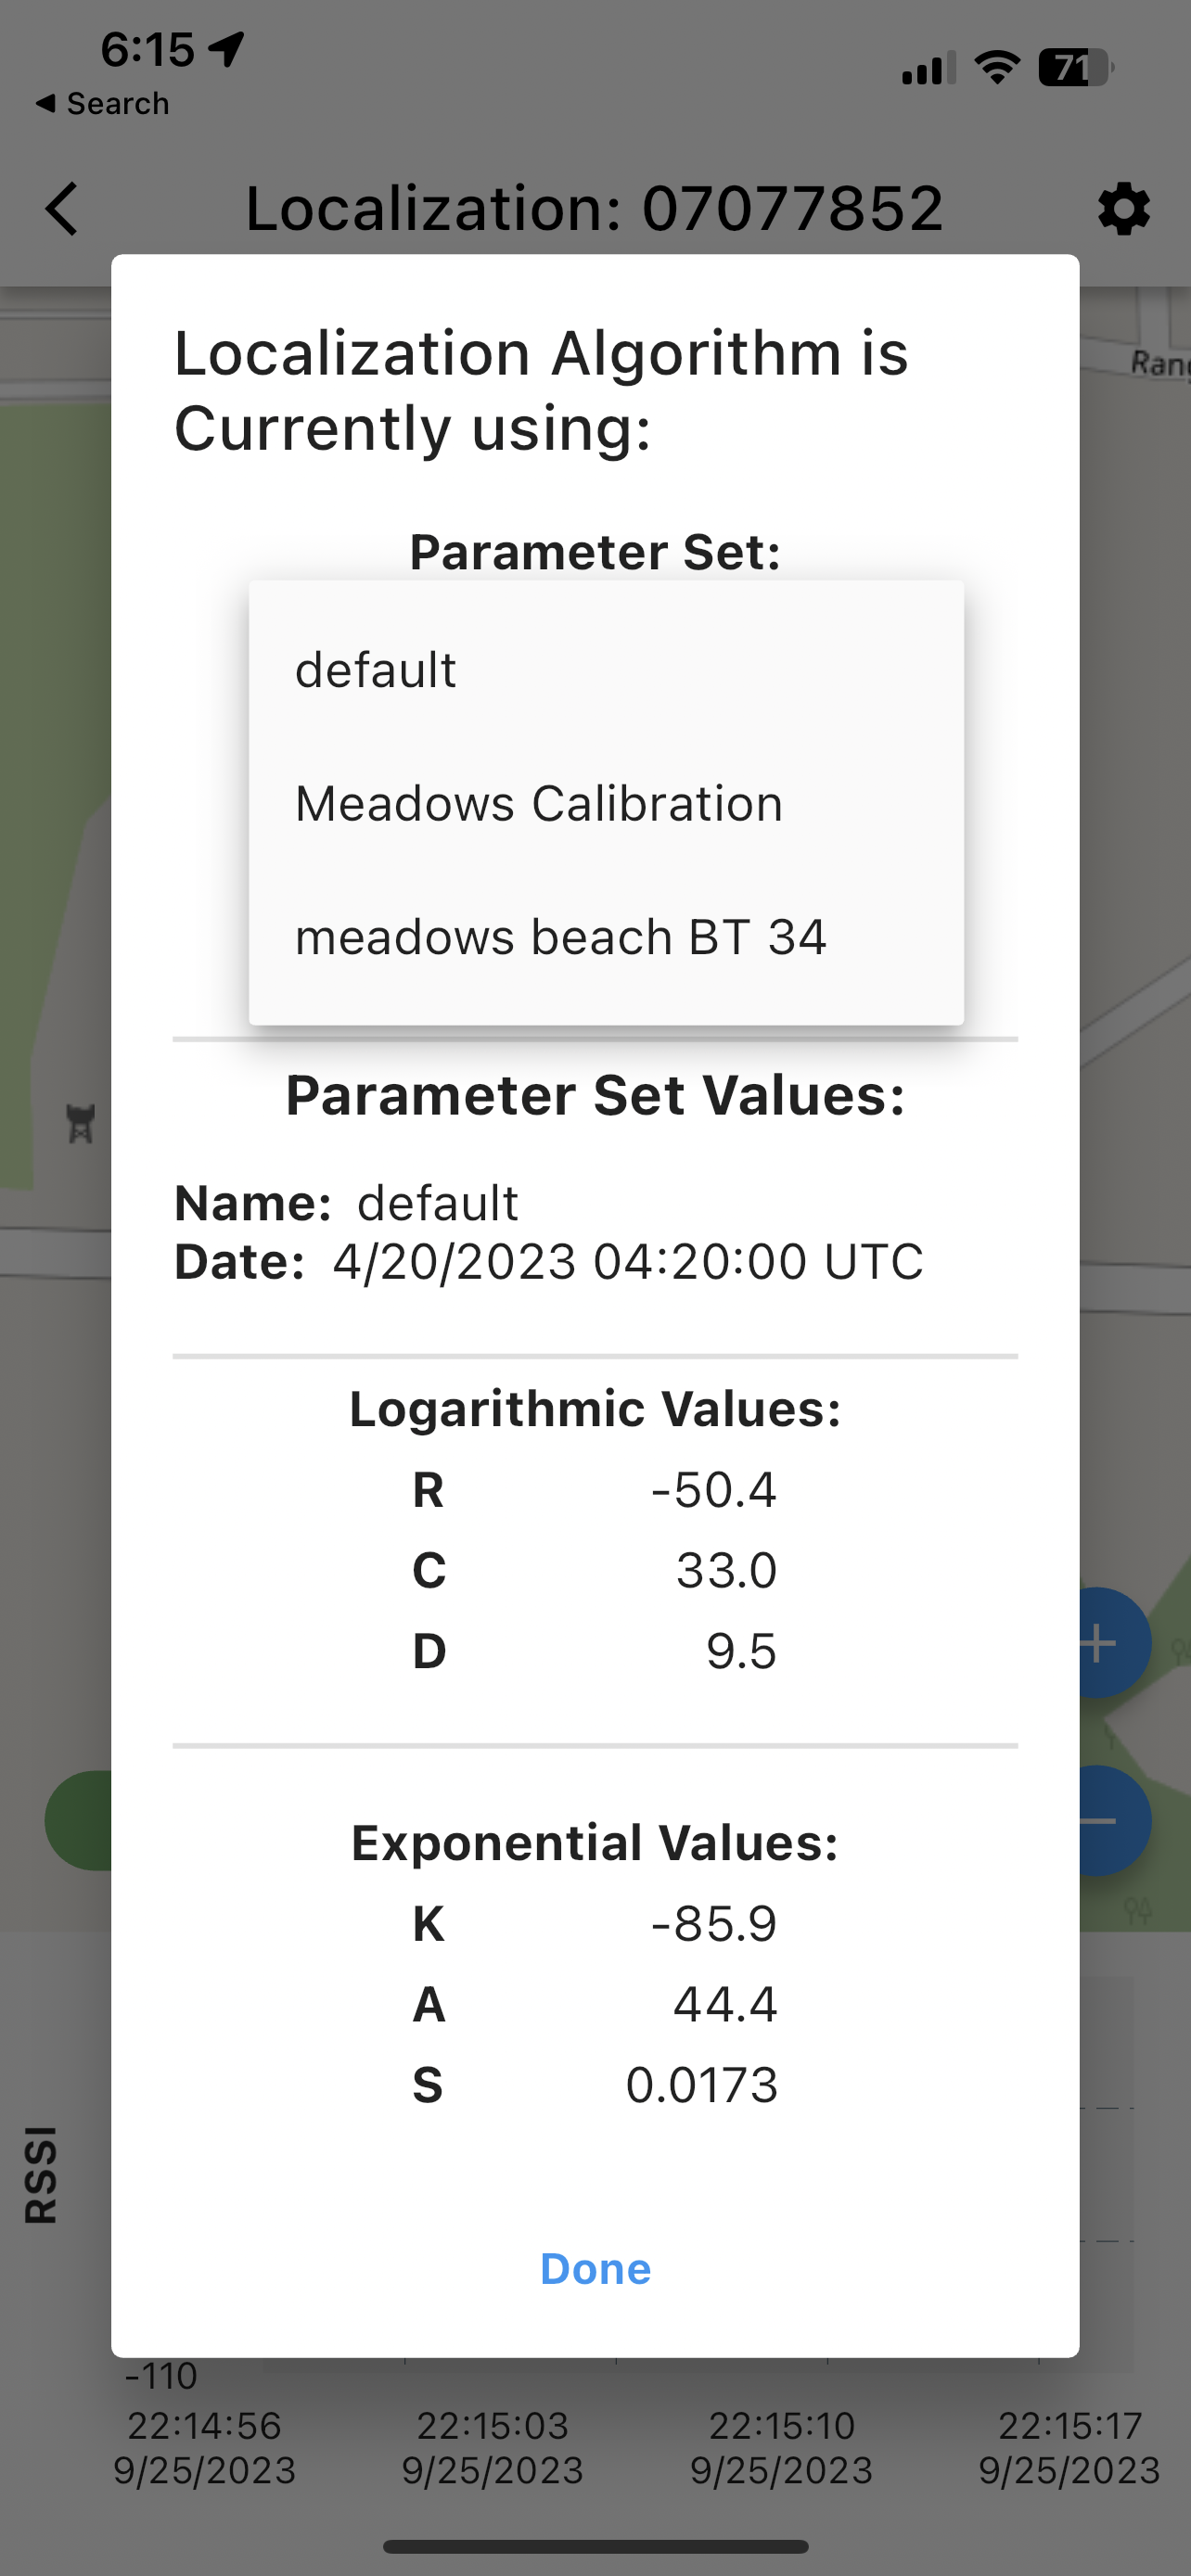
\includegraphics[width=0.25\textwidth,height=\textheight]{./images/sk_localization_chooseParam.PNG}
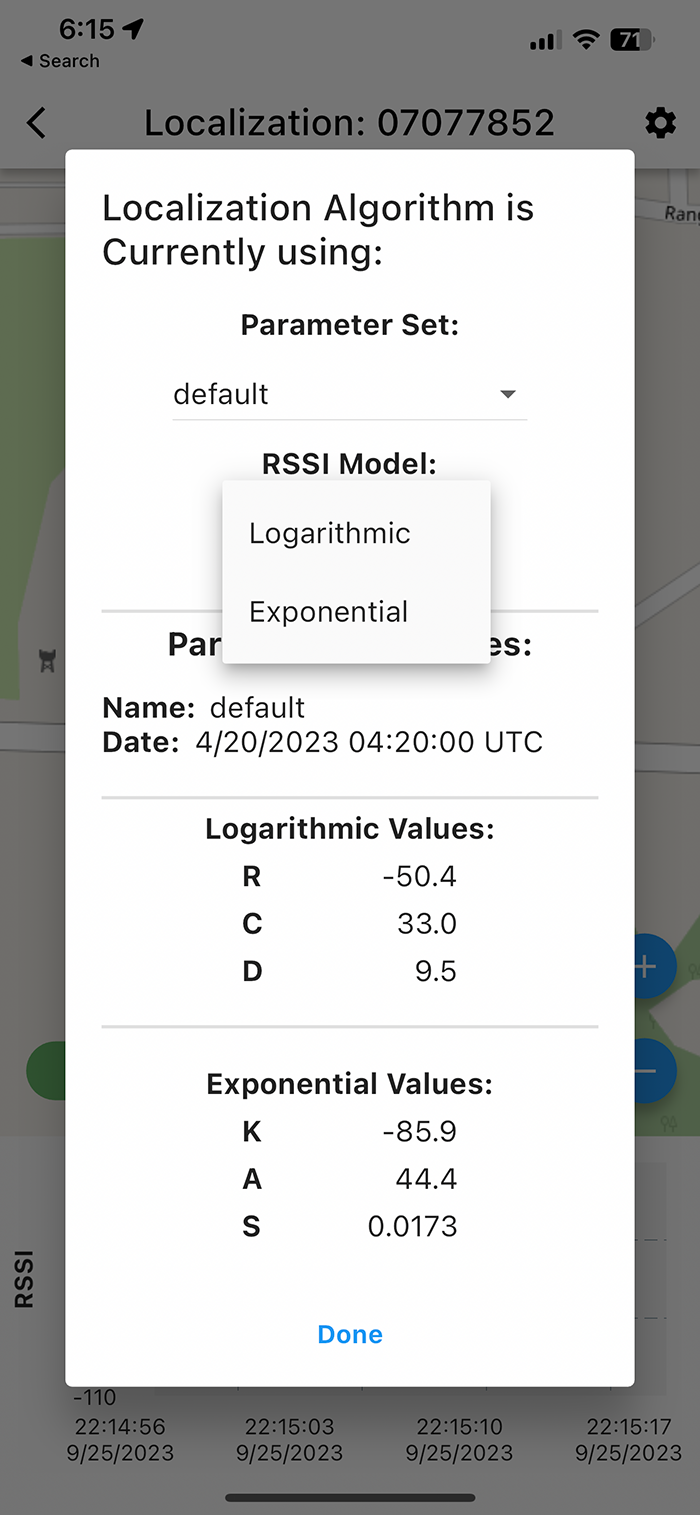
\includegraphics[width=0.25\textwidth,height=\textheight]{./images/sk_localization_chooseModel.PNG}
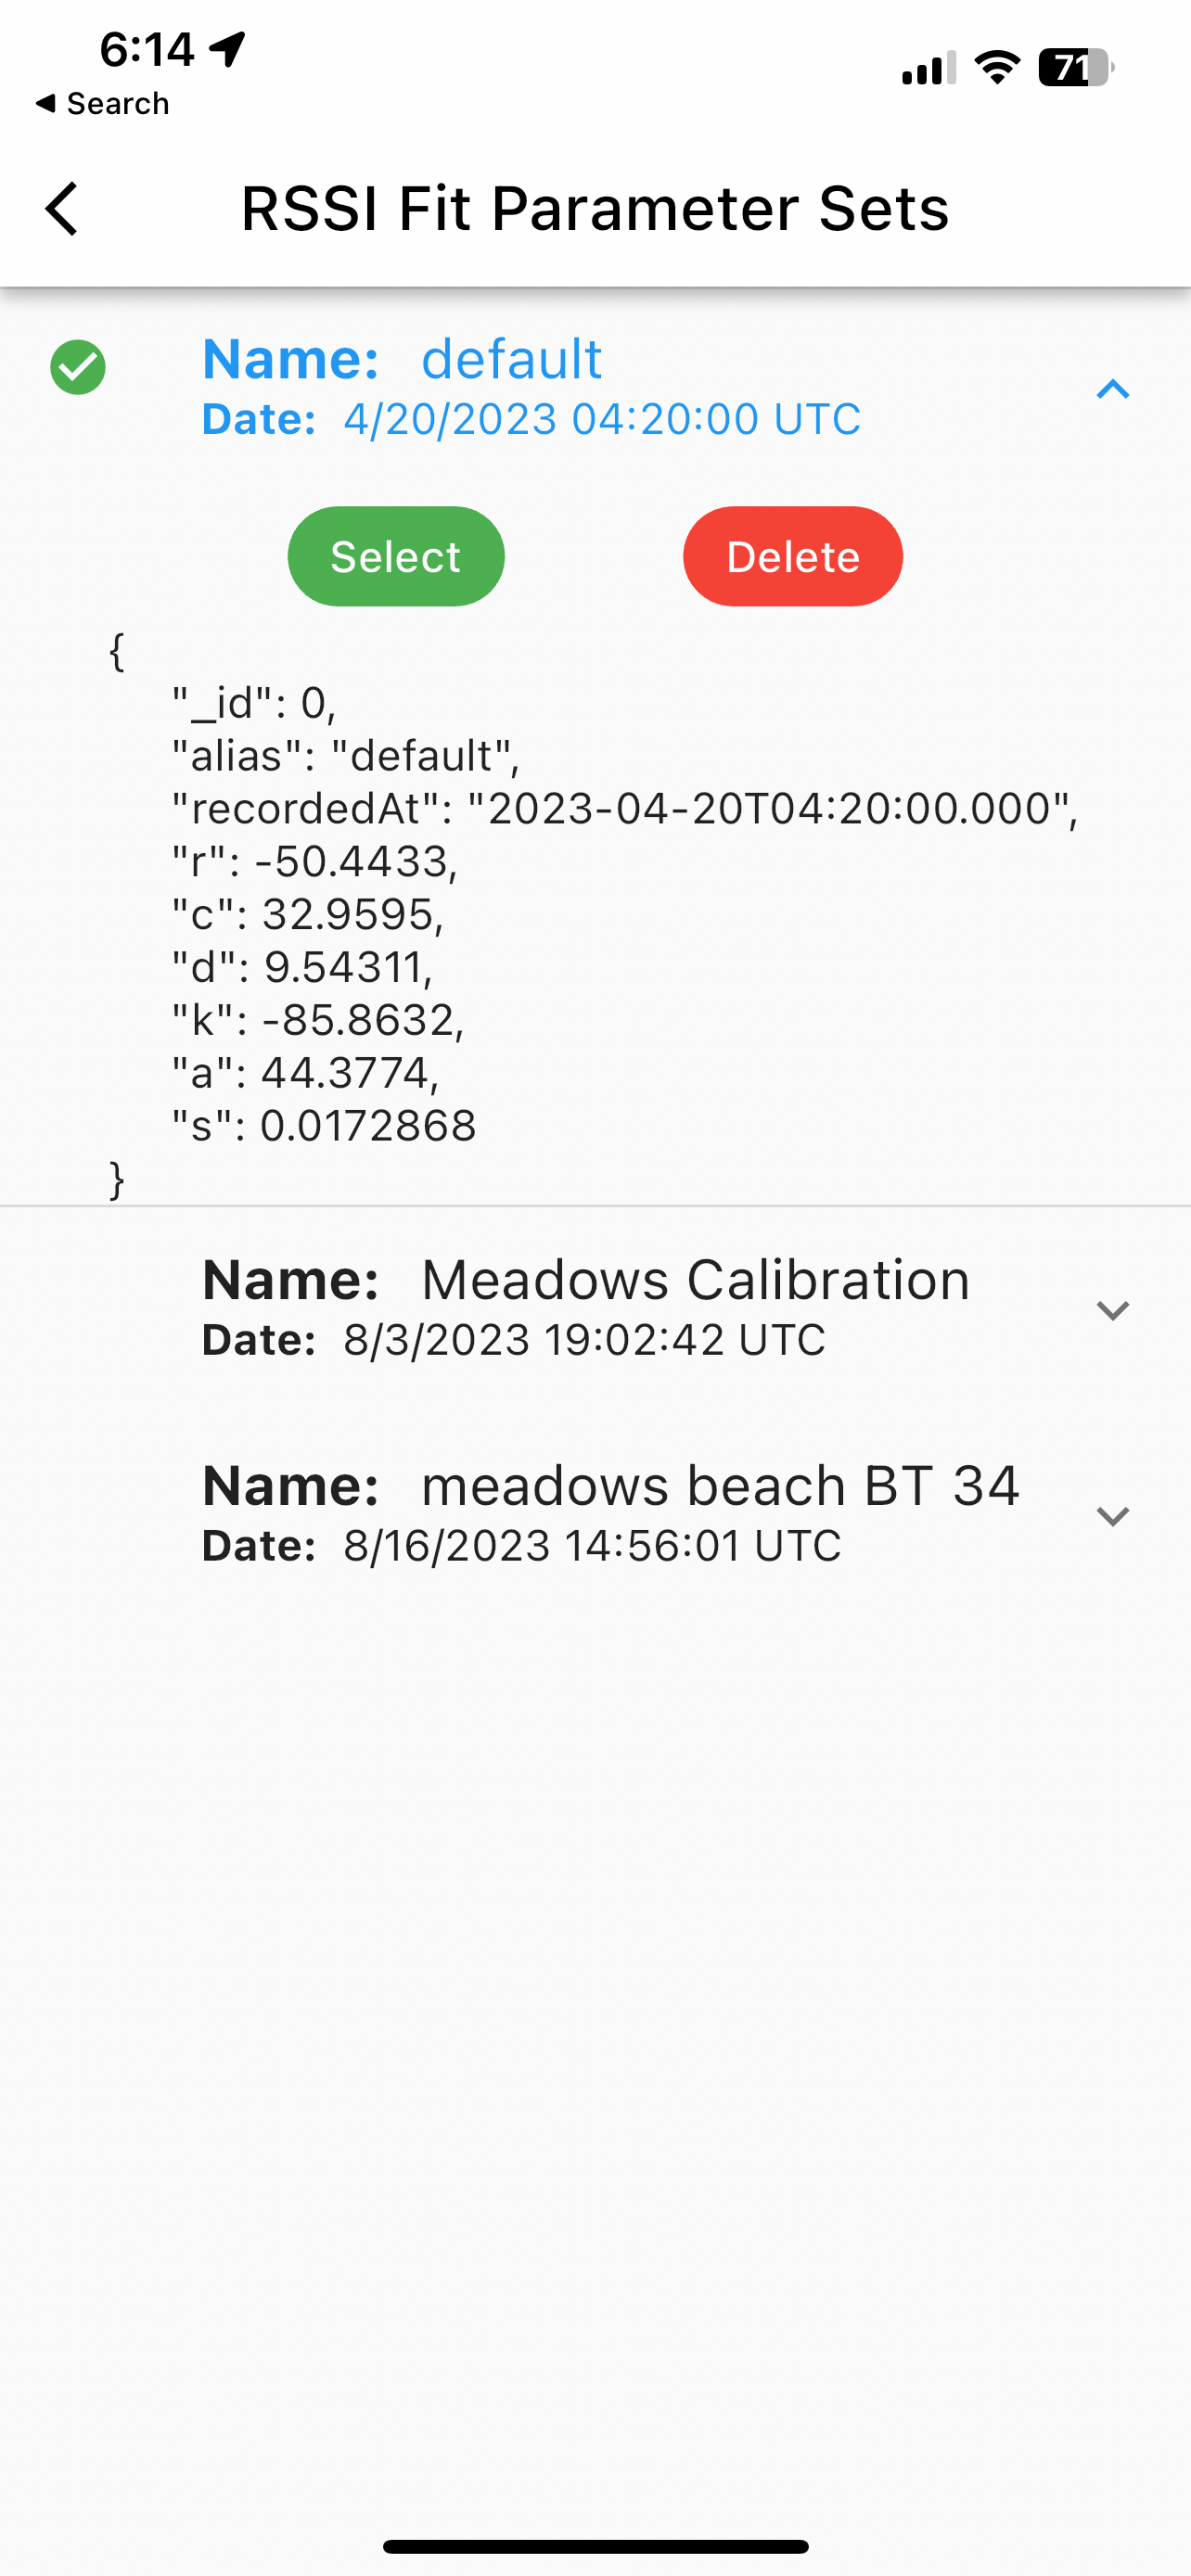
\includegraphics[width=0.25\textwidth,height=\textheight]{./images/sk_localization_paramDesc.PNG}
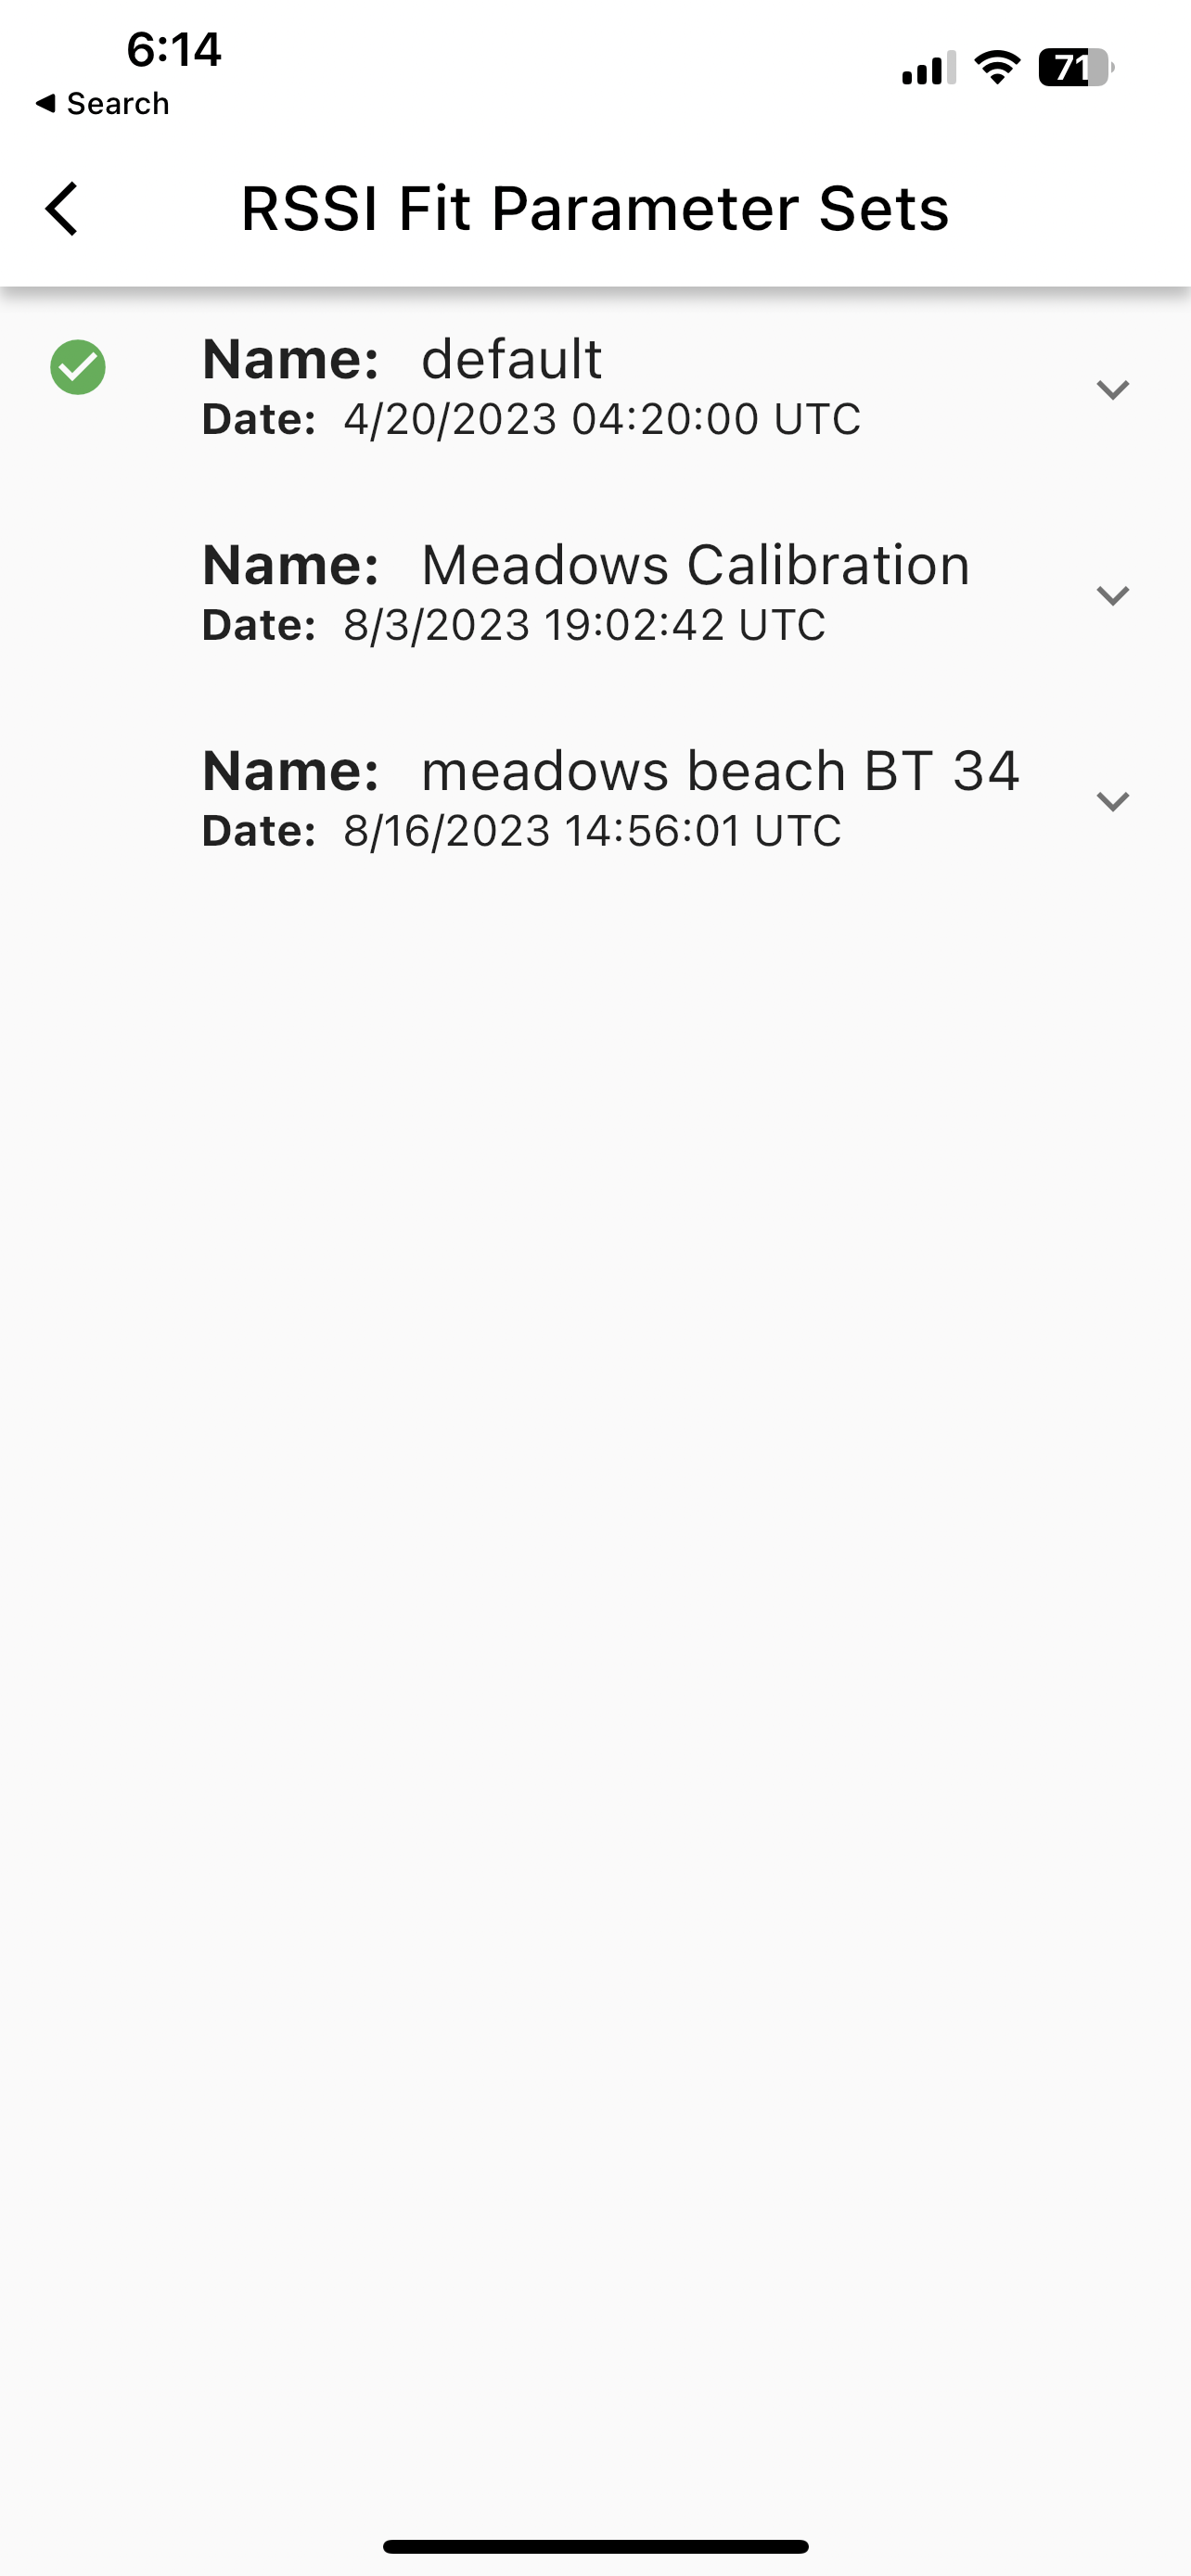
\includegraphics[width=0.25\textwidth,height=\textheight]{./images/sk_localization_ParamSets.PNG}

\hypertarget{firmware-updates}{%
\subsection{Firmware Updates}\label{firmware-updates}}

\textbf{Coming Soon}

\hypertarget{final-thoughts}{%
\section{Final Thoughts}\label{final-thoughts}}

This User Guide is a living document. Your experiences and input are
greatly appreciated so please don't hesitate to reach out to us
regarding what you'd like to see included here. You can submit your
suggestions and any errors to our \texttt{Customer\ Service\ Desk}
\href{https://celltracktech.com/pages/customer-service-desk-csd}{here}
and we will work to incorporate them in future revisions. All material ©
Cellular Tracking Technologies, 2023.

\newpage

\end{document}
